\documentclass[12pt]{book}
\usepackage[a4paper,bindingoffset=0.2in,%
            left=0.75in,right=0.75in,top=1in,bottom=1in,%
            footskip=.25in]{geometry}
\usepackage{fancyhdr}
\setlength{\headheight}{15.2pt}
\usepackage[utf8]{inputenc}
\pagestyle{fancy}

\renewcommand{\chaptermark}[1]{\markboth{\thechapter.\ #1}{}}
\renewcommand{\sectionmark}[1]{\markright{\thesection\ #1}}
\fancyhead[LE,RO]{\textbf{\thepage}}
\fancyhead[LO]{\textbf{\rightmark}}
\fancyhead[RE]{\textbf{\leftmark}}
\fancyfoot{}
\fancypagestyle{plain}
{
    \fancyhf{}
}


\usepackage{amsmath}
\usepackage{amssymb}
\usepackage{mathtools}
\usepackage{xcolor}
\usepackage{enumitem}


\usepackage{common}
\usepackage{english-theorems}
\setcounter{tocdepth}{1}

%\DeclareMathOperator*{\accept}{acc}
%\DeclareMathOperator*{\reject}{rej}

\begin{document}
\tableofcontents
\clearpage
\ifodd\value{page}\else
\thispagestyle{empty}
\fi
% \part{Quantum Mechanic: Done Right}
\chapter{Schr\"{o}dinger's Equation and Wavefunction}
\section{Introduction}
In classical mechanic, the state of a wave is represented by a function \(\func{\Psi}{\vectbf{r},t}\) which satisfies
\begin{equation*}
    \Delta \func{\Psi}{\vectbf{r},t} = \frac{1}{v^2} \dfrac{\partial^2}{\partial t^2} \func{\Psi}{\vectbf{r},t}
\end{equation*}
for some constant \(v\) wtih dimension of speed. Note that, due to that fact that both sides are second derivative, the equation does not have any imaginary parts for the plane waves \(\func{\Psi}{\vectbf{r},t} = e^{- i(\omega t - \vectbf{k} \cdot \vectbf{r})}\) where \(\omega= 2\pi \nu\) is the angular frequency and \(\vectbf{k}\) is the wave vector such that \(\abs{\vectbf{k}} = \frac{2\pi}{\lambda}\) with \(\lambda\) denoting wave length.

Einstein and Plank postulated that for a photon
\begin{align}\label{eq:duality}
    E & = h \nu = \hbar \omega & \vectbf{p} & = \hbar \vectbf{k}
\end{align}
To describe a wave we need its frequency and wavelength and to describe a particle we need its momentum energy. Therefore, these equations \ref{eq:duality} imply the dual nature of light as a wave and a particle. When light has no interaction it propagates as a wave and when it interacts its particle nature appears. De Broglie stated that equations \ref{eq:duality} holds for both light and matter. That is, a moving particle behaves like a wave -- a stationary particle does not have a wave nature. Since moving particles act like a wave, then there must be a wave function for that particle, Schr\"{o}dinger postulated.

Thus, the states in quantum mechanic are denoted by a wavefunction \(\func{\Psi}{\vectbf{r},t}\). The wavefunction \(\Psi\) must satisfy the Schr\"{o}dinger's equation.
\begin{equation*}
    -\dfrac{\hbar^2}{2m} \Delta \func{\Psi}{\vectbf{r},t} + \func{V}{\vectbf{r},t} \func{\Psi}{\vectbf{r},t} = -i\hbar \dfrac{\partial}{\partial t} \func{\Psi}{\vectbf{r},t}
\end{equation*}
Schr\"{o}dinger realized that is necessary to only consider the first time derivative, so that the Broglie's equations hold. However, this means that the wavefunction has some imaginary part. Moreover, we impose the following regularity conditions on \(\Psi\).
\begin{enumerate}
    \item \(\func{\Psi}{\vectbf{r},t} \in \Complex\).
    \item \(\Psi\) is continuous and single-valued.
    \item The partials \(\frac{\partial \Psi}{\partial x},\frac{\partial \Psi}{\partial y},\frac{\partial \Psi}{\partial z}\) are all continuous and single-valued.
    \item \(\Psi\) is square integrable, i.e.
          \begin{equation*}
              \int \abs{\Psi}^2 \diffOperator \vectbf{r}< + \infty
          \end{equation*}
          and thus, \(\lim_{x \to \pm \infty} \Psi = \lim_{y \to \pm \infty} \Psi = \lim_{z \to \pm \infty} \Psi = 0\).
\end{enumerate}

The operator \(H = -\frac{\hbar^2}{2m} \Delta + \func{V}{\vectbf{r},t}\) is called the \textbf{Hamiltonian operator} of the system, \(E = i\hbar \frac{\partial}{\partial t}\) is the \textbf{energy operator}, and \(P = -i\hbar \nabla\) is the \textbf{momentum operator}. The Schr\"{o}dinger equation can be written as
\begin{equation*}
    H \func{\Psi}{\vectbf{r},t} = \bracket{ \frac{P^2}{2m}  + \func{V}{\vectbf{r},t}} \func{\Psi}{\vectbf{r},t} = E \func{\Psi}{\vectbf{r},t}
\end{equation*}

Since there is no complex wave in nature, Born's stated that the \(\abs{\func{\Psi}{\vectbf{r},t}}^2\) represents the probability that the particle is at \(\vectbf{r}\) at time \(t\). As a result, we may assume that that \(\func{\Psi}{\vectbf{r},t}\) is normalized, that is
\begin{equation*}
    \int \abs{\func{\Psi}{\vectbf{r},t}}^2 \diffOperator \vectbf{r} = 1
\end{equation*}

The expected value of a quantity \(\func{f}{\vectbf{r},\vectbf{p},t}\) is calculated as
\begin{equation*}
    \angleBracket{\func{f}{\vectbf{r},\vectbf{p},t}} = \int \overline{\func{\Psi}{\vectbf{r},t}} \func{f}{\vectbf{r},-i\hbar \nabla,t} \func{\Psi}{\vectbf{r},t} \diffOperator \vectbf{r}
\end{equation*}

\begin{remark}
    The Schr\"{o}dinger equation does is not derived by some physical principle, but rather itself is taken as a postulate. Its correctness is not deduced from any experiment, however, it correctly predicts results of those experiments. A plausiblity argument can be given for the Schr\"{o}dingers equation, that uses four assumptions about properties of quantum wave function.
    \begin{enumerate}
        \item It must be consistent with De Broglie equations.
        \item It must be consistent with the equation
              \begin{equation*}
                  E = \frac{p^2}{2m} + V
              \end{equation*}
        \item The equation describing \(\Psi\), must be linear in \(\Psi\) to allow for wave interferences.
        \item The potential energy of the system only depends on \(\vectbf{r}\) and \(t\).
    \end{enumerate}
\end{remark}

\subsection*{Hisenberg's uncertainty principle}
In classical mechanic, the Fourier transform of a wave \(\func{f}{t}\) is \(\func{F}{\omega}\) and the bandwidths satisfy \(\Delta t \Delta \omega \geq \frac{1}{2}\). Similarly, for a spatial wave, \(t\) is replace with \(\vectbf{r}\) and \(\omega\) with \(\vectbf{k}\). The \((t,\omega)\) and \((\vectbf{r}, \vectbf{k})\) are called conjugate pairs. From the De Broglie's equations we know that \(\vectbf{p} \propto \vectbf{k}\) and hence \((\vectbf{r}, \vectbf{p})\) are conjugate pairs, as well.
\begin{align*}
    \func{\overline{\Psi}}{\vectbf{p},t} & = \bracket{\dfrac{1}{2\pi \hbar}}^{\frac{3}{2}} \int \func{\Psi}{\vectbf{r},t} e^{-i \vectbf{p} \cdot \vectbf{r}/\hbar}\diffOperator \vectbf{r}           \\
    \func{\Psi}{\vectbf{r},t}            & = \bracket{\dfrac{1}{2\pi \hbar}}^{\frac{3}{2}} \int \func{\overline{\Psi}}{\vectbf{p},t} e^{i \vectbf{p} \cdot \vectbf{r}/\hbar}\diffOperator \vectbf{p}
\end{align*}
Then, we can arrive at the Hisenberg's uncertainty principle as follows:
\begin{align*}
    \Delta \vectbf{r} \Delta \vectbf{p} & = \hbar\Delta \vectbf{r} \Delta  \vectbf{k} \geq \dfrac{\hbar}{2} \\
    \Delta t \Delta E                   & = \hbar \Delta t \Delta  \nu \geq \dfrac{\hbar}{2}
\end{align*}
The Bohr's complementary principle states that an experiment that forces the quantum state to reveal its wave nature strongly suppresses its particle nature and vice verse. Therefore, the results of a quantum experiment depends on the observer.

\section{Time independent Schr\"{o}dinger equation}
Most systems in quantum mechanic have time independent potential \(\func{V}{\vectbf{r}, t} = \func{V}{\vectbf{r}}\). Moreover, we then assume that \(\func{\Psi}{\vectbf{r},t} = \func{\psi}{\vectbf{r}} \func{\phi}{t}\) is separable. Then we have,
\begin{align*}
     & -\frac{\hbar^2}{2m} \Delta \func{\psi}{\vectbf{r}} \func{\phi}{t} + \func{V}{\vectbf{r}} \func{\psi}{\vectbf{r}} \func{\phi}{t}  = i \hbar \dfrac{\partial}{\partial t} \func{\psi}{\vectbf{r}} \func{\phi}{t}           \\
     & -\frac{\hbar^2}{2m} \func{\phi}{t}\Delta \func{\psi}{\vectbf{r}} + \func{V}{\vectbf{r}} \func{\psi}{\vectbf{r}} \func{\phi}{t}  = i \hbar \func{\psi}{\vectbf{r}} \dfrac{\diffOperator}{\diffOperator t}  \func{\phi}{t}
\end{align*}
dividing both sides by \(\func{\psi}{\vectbf{r}} \func{\phi}{t}\) gives
\begin{equation*}
    -\frac{\hbar^2}{2m} \dfrac{1}{\func{\psi}{\vectbf{r}}}\Delta \func{\psi}{\vectbf{r}} + \func{V}{\vectbf{r}}  = i \hbar \frac{1}{\func{\phi}{t}} \dfrac{\diffOperator}{\diffOperator t}  \func{\phi}{t}
\end{equation*}
The left-hand side is a function of \(\vectbf{r}\) and the right-hand side is a function of \(t\) therefore, they must be equal to a constant \(G\).
\begin{equation*}
    i \hbar \frac{1}{\func{\phi}{t}} \dfrac{\diffOperator}{\diffOperator t}  \func{\phi}{t} = G \implies  \dfrac{\diffOperator}{\diffOperator t}  \func{\phi}{t} = -i \frac{G}{\hbar} \func{\phi}{t} \implies \func{\phi}{t} = A \func{\exp}{-i\frac{G}{\hbar} t}
\end{equation*}
for some constant \(A\) -- We may assume \(A = 1\). We know that the angular frequency is \(\omega = \frac{G}{\hbar}\) and \(E = \hbar \omega\) thus, \(G = E\). Then,
\begin{equation*}
    -\frac{\hbar^2}{2m} \Delta \func{\psi}{\vectbf{r}} + \func{V}{\vectbf{r}}\func{\psi}{\vectbf{r}} = E\func{\psi}{\vectbf{r}}
\end{equation*}
If some \(\psi\) satisfies the above's equation for some given potential, then \(\func{\psi}{\vectbf{r}} \func{\exp}{- i \frac{E}{\hbar} t}\) is a solution of the system.
\subsection{Particle in an infinite potential well}
Suppose the following potential is given
\begin{equation*}
    \func{V}{x} = \begin{cases}
        0      & 0 \leq x \leq L  \\
        \infty & \text{otherwise}
    \end{cases}
\end{equation*}
Intuitively, the particle is bounded in \(\clcl{0}{L}\) and it is imposible to find it outside of this box. Thus, we may only consider the solutions on the equation on \(\clcl{0}{L}\).
\begin{equation*}
    -\frac{\hbar^2}{2m} \dfrac{\diffOperator^2}{\diffOperator x^2} \func{\psi}{x} = E \func{\psi}{x} \implies \func{\psi}{x} = A \func{\cos}{\dfrac{\sqrt{2Em}}{\hbar} x + \theta}
\end{equation*}
with boundary conditions \(\func{\psi}{0} = \func{\psi}{L} = 0\).
\begin{align*}
     & \func{\psi}{0} = A \func{\cos}{\theta} = 0 \implies \theta = -\frac{\pi}{2} \implies \func{\psi}{x} = A \func{\sin}{\dfrac{\sqrt{2Em}}{\hbar} x} \\
     & \func{\psi}{L} = A \func{\sin}{\dfrac{\sqrt{2Em}}{\hbar} L} = 0 \implies \dfrac{\sqrt{2Em}}{\hbar}L = \pi n
\end{align*}
This implies that energy is quantized as
\begin{equation*}
    E_n = \dfrac{\pi^2 \hbar^2 n^2}{2L^2m}
\end{equation*}
Then,
\begin{equation*}
    \func{\psi_n}{x} = A_n \func{\sin}{\dfrac{\sqrt{2E_n m}}{\hbar} x} = A_n \func{\sin}{\dfrac{n \pi}{L} x}
\end{equation*}
and for \(A_n\)
\begin{align*}
    \int_{0}^L \abs{\func{\psi_n}{x}}^2 \diffOperator x & =  A_n^2 \int_{0}^L \func{\sin^2}{\dfrac{n \pi}{L} x}\diffOperator x                         \\
                                                        & = A_n^2 \evaluate{\dfrac{x}{2} - L\dfrac{\func{\sin}{2 \frac{n \pi}{L} x }}{4 \pi n} }_{0}^L \\
                                                        & = A_n^2 \frac{L}{2} = 1                                                                      \\
    \implies                                            & A_n = \sqrt{\frac{2}{L}}
\end{align*}
\subsection{Particle in an finite potential well}
The potential is given by
\begin{equation*}
    \func{V}{x} = \begin{cases}
        V & x < 0 \lor x > L \\
        0 & 0 \leq x \leq L
    \end{cases}
\end{equation*}
and the wavefunction satisfies.
\begin{equation*}
    -\frac{\hbar^2}{2m} \dfrac{\diffOperator^2}{\diffOperator x^2} \func{\psi}{x} + \func{V}{x}\func{\psi}{x}= E \func{\psi}{x}
\end{equation*}
If \(E > V\), then the wavefunctions are not square-integrable and as a result the spectrum is continuous. Suppose \(E < V\), in the region I -- \(x < 0\),-- the wavefunction is given by 
\begin{equation*}
    \frac{\hbar^2}{2m} \dfrac{\diffOperator^2}{\diffOperator x^2} \func{\psi_I}{x} = (V - E)\func{\psi_I}{x} \implies \func{\psi_I}{x} = A e^{\alpha x} + B e^{- \alpha x}
\end{equation*}
where \(\alpha=  \sqrt{\frac{2m(V - E)}{\hbar^2}}\). As \(x \to -\infty\), we must have \(\func{\psi_I}{x} \to 0\) hence \(B = 0\). Similarly, for region III -- \(x > L\), -- the wavefunction is given by 
\begin{equation*}
    \frac{\hbar^2}{2m} \dfrac{\diffOperator^2}{\diffOperator x^2} \func{\psi_{III}}{x} = (V - E)\func{\psi_{III}}{x} \implies \func{\psi_{III}}{x} = C e^{\alpha x} + D e^{- \alpha x}
\end{equation*}
As \(x \to \infty\), we must have \(\func{\psi_{III}}{x} \to 0\) hence \(C = 0\). Lastly, for region II -- \(0 \leq x \leq L\),-- the wavefunction is given by 
\begin{equation*}
    \frac{\hbar^2}{2m} \dfrac{\diffOperator^2}{\diffOperator x^2} \func{\psi_{II}}{x} = -E\func{\psi_{II}}{x} \implies \func{\psi_{II}}{x} = E e^{i\beta x} + F e^{- i\beta x}
\end{equation*}
where \(\beta = \sqrt{\frac{2mE}{\hbar^2}}\). Note that \(\psi\) and its derivative are both continuous. Setting up those equation allows us to eliminate some of these constants. 
\begin{align*}
    \func{\psi_{I}}{0} &= \func{\psi_{II}}{0} \implies A = E + F\\
    \frac{\diffOperator}{\diffOperator x}\func{\psi_{I}}{0} &= \frac{\diffOperator}{\diffOperator x}\func{\psi_{II}}{0} \implies A = \frac{i\beta}{\alpha} \bracket{E - F}\\
    \implies& E = A \bracket{\frac{1}{2} - i \frac{\alpha}{2\beta} } \ \ F = A \bracket{\frac{1}{2} + i \frac{\alpha}{2\beta} }\\
    \implies& \func{\psi_{II}}{x} = A \func{\cos}{\beta x} + A \frac{\alpha}{\beta} \func{\sin}{\beta x}\\
    \func{\psi_{II}}{L} &= \func{\psi_{III}}{L} \implies D = A e^{\alpha L}\func{\cos}{\beta L} + A \frac{\alpha}{\beta} e^{\alpha L}\func{\sin}{\beta L}\\
    \frac{\diffOperator}{\diffOperator x}\func{\psi_{II}}{L} &= \frac{\diffOperator}{\diffOperator x}\func{\psi_{III}}{L} \implies  D = - A e^{\alpha L}\func{\cos}{\beta L} + A \frac{\beta}{\alpha} e^{\alpha L}\func{\sin}{\beta L}\\
    \implies & \tan \beta L = \frac{2\alpha \beta}{\beta^2 - \alpha^2}
\end{align*}
The last equation allows to get the values of \(E\). Although, there are no analytic closed form for the values of \(E\), we can see that they are discrete. 
\subsection{Harmonic oscillator}
The potential is given by \(\func{V}{x} = \frac{1}{2}Cx^2\) where \(C = m \omega^2\), \(\omega\) being the angular frequency.
\begin{equation*}
    \bracket{ \dfrac{\diffOperator^2}{\diffOperator x^2}  + \frac{1}{2}m\omega^2 x^2 - E} \func{\psi}{x} = -\frac{\hbar^2}{2m} \bracket{ \dfrac{\diffOperator^2}{\diffOperator x^2}  - \frac{m^2 \omega^2}{\hbar^2} x^2 + \dfrac{2mE}{\hbar^2}} \func{\psi}{x} = 0
\end{equation*}
Let \(\alpha = \frac{m \omega}{\hbar}\) and \(\beta = \frac{2mE}{\hbar^2}\), then
\begin{equation*}
    \frac{\diffOperator^2}{\diffOperator x^2} \func{\psi}{x} + \bracket{\beta - \alpha^2 x^2}\func{\psi}{x} = 0
\end{equation*}
Consider the change of variable \(u = \sqrt{\alpha}x\), then
\begin{equation*}
    \frac{\diffOperator^2}{\diffOperator x^2} =\bracket{\dfrac{\diffOperator}{\diffOperator u} \dfrac{\diffOperator u}{\diffOperator x}} \bracket{\dfrac{\diffOperator}{\diffOperator u} \dfrac{\diffOperator u}{\diffOperator x}} = \alpha \dfrac{\diffOperator^2}{\diffOperator u^2}
\end{equation*}
which gives
\begin{equation*}
    \frac{\diffOperator^2}{\diffOperator u^2} \func{\psi}{u} + \bracket{\frac{\beta}{\alpha} - u^2}\func{\psi}{u} = 0
\end{equation*}
Note that for sufficiently large \(u\) we can approximate the behaviour of \(\func{\psi}{u}\) as
\begin{equation*}
    \frac{\diffOperator^2}{\diffOperator u^2} \func{\psi}{u} -  u^2\func{\psi}{u} = 0 \implies \func{\psi}{u} \asymp  e^{-u^2/2}
\end{equation*}
Let \(\func{H}{u}\) be the lower degree terms in \(\func{\psi}{u}\), i.e. \(\func{\psi}{u} = \func{H}{u} e^{-u^2/2} \) and let \(\gamma = \frac{\beta}{\alpha} = \frac{E}{\hbar \omega}\). By substituting \(\func{\psi}{u} = \func{H}{u}e^{-u^2/2}\) we get
\begin{align*}
     & \frac{\diffOperator^2}{\diffOperator u^2}\func{H}{u} e^{-\frac{u^2}{2}} +  \bracket{\gamma - u^2} \func{H}{u} e^{-\frac{u^2}{2}}                                                                                                  \\
     & = \bracket{\frac{\diffOperator^2}{\diffOperator u^2}\func{H}{u} - 2u \frac{\diffOperator}{\diffOperator u}\func{H}{u} + \bracket{u^2 - 1} \func{H}{u}}  e^{-\frac{u^2}{2}} + \bracket{\gamma - u^2}\func{H}{u} e^{-\frac{u^2}{2}} \\
     & = \bracket{\frac{\diffOperator^2}{\diffOperator u^2}\func{H}{u} - 2u \frac{\diffOperator}{\diffOperator u}\func{H}{u} + \bracket{\gamma - 1}\func{H}{u} } e^{-\frac{u^2}{2}} = 0                                                  \\
     & \implies  \frac{\diffOperator^2}{\diffOperator u^2}\func{H}{u} - 2u \frac{\diffOperator}{\diffOperator u}\func{H}{u} + \bracket{\gamma - 1}\func{H}{u} = 0
\end{align*}
We employ the power series technique to find \(\func{H}{u}\). Substitute \(\func{H}{u} = \sum_{n = 0}^{\infty} h_n u^n\)
\begin{align*}
     & \frac{\diffOperator^2}{\diffOperator u^2}\func{H}{u} - 2u \frac{\diffOperator}{\diffOperator u}\func{H}{u} + \bracket{\gamma - 1}\func{H}{u} \\
     & = \sum_{n = 0}^{\infty} n \bracket{n-1} h_n u^{n-2} - 2u n h_n u^{n-1} + \bracket{\gamma - 1} h_n u^n                                        \\
     & = \sum_{n = 0}^{\infty} \squareBracket[[\Bigg]]{\bracket{n+2}\bracket{n+1} h_{n+2} - 2 n h_{n} + \bracket{\gamma - 1} h_n}u^n                \\
     & = \sum_{n = 0}^{\infty} \squareBracket[[\Bigg]]{\bracket{n+2}\bracket{n+1} h_{n+2} +  \bracket{\gamma -2 n- 1} h_n}u^n = 0                   \\
     & \implies h_{n+2} = \dfrac{2n + 1 - \gamma}{\bracket{n+2}\bracket{n+1}} h_n                                                                   \\
     & \implies \begin{cases}
                    h_{2n}     & = \dfrac{\prod_{k=1}^n (4k - 3 -\gamma)}{(2n)!} h_0      \\
                    h_{2n + 1} & = \dfrac{\prod_{k=1}^n (4k - 1  -\gamma)}{(2n + 1)!} h_1 \\
                \end{cases}
\end{align*}
for \(n \geq 1\) and arbitrary \(h_0,h_1\). Let \(\func{H_0}{u}\) and \(\func{H_1}{u}\) be the even and odd component of \(\func{H}{u}\) as such
\begin{equation*}
    \func{H}{u} = h_0 \bracket{1 + \frac{h_2}{h_0} u^2 + \dots } + h_1u \bracket{1 + \frac{h_3}{h_1} u^2 + \dots } = h_0 \func{H_0}{u} + h_1u \func{H_1}{u}
\end{equation*}
If \(\gamma \neq 4k - 3\) for some \(k \geq 1\), then the coefficients of \(\func{H_0}{u}\) grow the same as \(e^{-u^2/2}\). Similary, if \(\gamma \neq 4k - 1\) for some \(k \geq 1\), then the coefficients of \(\func{H_1}{u}\) grow the same as \(e^{-u^2/2}\). However, both of these contradict the fact that \(\func{H}{u}\) is of lower degree than \(e^{-u^2/2}\). Therefore, we must either have \(\gamma = 4k - 3\) and \(h_1 = 0\) or \(\gamma = 4k - 1\) and \(h_0 = 0\). As a result, \(\gamma = 2n + 1\) for \(n \geq 0\) and thus \(E = \bracket{n + \frac{1}{2}} \hbar \omega\). Moreover, we get the following table for the possible Hermite polynomials
\begin{center}
    \begin{tabular}{c|c|c}
        \(n\) & \(\func{H_0}{u}\) & \(u\func{H_1}{u} \)\\ \hline 
        0 & \(1\) & \\ \hline 
        1 &  & \(u\) \\ \hline 
        2 & \(1 - u^2\) & \\\hline 
        3 &  & \(3u - 2 u^3\) \\\hline
        4 & \(3 - 12 u^2 + 4u^4\) &  \\\hline 
        5 & & \(15u - 20u^3 + 4u^5\) \\
    \end{tabular}
\end{center}
we then get the following wavefunctions
\begin{equation*}
    \func{\psi_n}{x} = A_n \func{H_n}{\sqrt{\frac{m\omega}{\hbar} x}} \func{\exp}{- \frac{m\omega x^2}{2\hbar}} = \dfrac{1}{\sqrt{2^n n!}} \bracket{\dfrac{m\omega}{\pi \hbar}}^{1/4} \func{H_n}{\sqrt{\frac{m\omega}{\hbar} x}} \func{\exp}{- \frac{m\omega x^2}{2\hbar}}
\end{equation*}
where \(\func{H_n}{u}\) is the physicist's Hermite polynomials.
\begin{center}
    \begin{tabular}{c|l}
        \(n\) & \(\func{H_n}{u}\) \\ \hline 
        0 & \(1\)  \\ \hline 
        1 &  \(u\) \\ \hline 
        2 & \(4u^2 - 2\)  \\\hline 
        3 &   \(8u^3 - 12 u\) \\\hline
        4 & \(16u^4 - 48u^2 + 12 3\)  \\\hline 
        5 &  \(32u^5 - 160u^3 + 120u\) \\
    \end{tabular}
\end{center}
\chapter{Dirac Algebraic Formalism}
\section{Hilbert vector space}
Let \(\calL^2 = \func{\calL^2}{\Complex}\) be the set of all the square integrable complex functions \(\func{f}{\vectbf{r},t}\). Let \(\calW\) be the set of all the possible wavefunctions. Clearly, \(\calW \subset \calL^2\).
\begin{proposition}
    \(\calL^2\) is Hilbert space and \(\calW\) is vector subspace of \(\calL^2\).
\end{proposition}
\begin{definition}
    Define the inner product \(\angleBracket{\Psi,\Phi}\) for all \(\Psi, \Phi \in \calL^2\) as
    \begin{equation*}
        \angleBracket{\Phi,\Psi} = \int \overline{\func{\Phi}{\vectbf{r},t}} \func{\Psi}{\vectbf{r},t} \diffOperator \vectbf{r}
    \end{equation*}
    The integral converges if \(\Psi,\Phi \in \calW\) -- prove the convergence and the inner productness.

    If \(\angleBracket{\Psi,\Phi} = 0\), then they are called \textbf{orthogonal}.
\end{definition}

In a vector space \textbf{operators} map a vector to another vector. An operator \(A\) is \textbf{linear} if for all \(\Psi,\Phi \in \calL^2\) and \(\lambda \in \Complex\)
\begin{equation*}
    \func{A}{\Psi + \lambda \Phi} = A \Psi + \lambda A \Phi
\end{equation*}

\begin{example}
    The following operators are linear
    \begin{enumerate}
        \item Parity operator \(\Pi \func{\Psi}{x,y,z,t} = \func{\Psi}{-x,-y,-z,t}\).
        \item \(X\) operator \(X \func{\Psi}{x,y,z,t} = x \func{\Psi}{x,y,z,t}\).
        \item \(D_x\) operator \(D_x \func{\Psi}{x,y,z,t} = \frac{\partial}{\partial x} \func{\Psi}{x,y,z,t}\).
    \end{enumerate}
\end{example}

\begin{definition}
    The \textbf{commutator} of two operators \(A\) and \(B\) is \(\commutator{A}{B} = AB - BA\). Similarly, the \textbf{anti-commutator} of two operators \(A\) and \(B\) is \(\anticommutator{A}{B} = AB + BA\).
\end{definition}

\begin{example}
    \(\commutator{X}{D_x} = -1\) and \(\commutator{X}{P} = i\hbar\).
\end{example}

\begin{definition}
    For any vector space we may find a \textbf{basis}; A set of linearly independent vectors that span the whole vector space. A basis \(\set{u_i}_{i \in I}\) -- \(u_i = \func{u_i}{\vectbf{r},t}\) -- is an orthonormal basis if
    \begin{equation*}
        \angleBracket{u_i,u_j} = \delta_{ij} = \begin{cases}
            1 & i = j              \\
            0 & \mathrm{otherwise}
        \end{cases}
    \end{equation*}
    where \(\delta_{ij}\) is the \textit{Kronecker delta}.
\end{definition}

If \(\set{u_i}_{i \in I}\) is basis for vector space \(V\), then all vectors \(v \in V\) can be represented uniquely as a linear combination of \(\set{u_i}\)
\begin{equation*}
    v = \sum_{i \in I} c_i u_i
\end{equation*}
Specifically, if \(\set{u_i}\) is basis for \(\calL^2\), then \(\Psi \in \calL^2\) can be represented as \(\Psi \equiv \bracket{c_i}_{i \in I}\).
If \(\Psi \equiv (c_i)\) and \(\Phi \equiv (d_i)\), then
\begin{equation*}
    \angleBracket{\Phi, \Psi} = \sum_{i \in I} c_i \overline{d_i}
\end{equation*}

The dual space \(V^{\ast}\) is the vector space containing all linear functionals \(\phi: V \to F\). Suppose \(\set{u_i}_{i \in I}\) is basis for a vector space \(V\) over the field \(F\). There exists a unique set of linearly independent vectors \(\set{u_i^{\ast}}_{i \in I} \subset V^{\ast}\) that makes a biorthogonal system with \(\set{u_i}\).
\begin{equation*}
    u^{\ast}_i u_j = \delta_{i,j}
\end{equation*}
The closure property states
\begin{equation*}
    \sum_{i \in I} u_i u_i^{\ast} = I
\end{equation*}
since for any \(v = \sum_{i \in I} c_i u_i\)
\begin{equation*}
    \operatorFunc{\sum_{i \in I} u_i u_i^{\ast}}{\sum_{i \in I} c_i u_i} = \sum_{i \in I}\sum_{j \in J} c_j u_i  u^{\ast}_i u_j = \sum_{i \in I} c_i u_i
\end{equation*}
\begin{remark}
    The dual set \(\set{u^{\ast}_i}\) does not necessarily span \(V^{\ast}\).
\end{remark}
If \(\set{u_i}\) is an orthonormal basis for \(\calL^2\), then
\begin{align*}
    \func{\Psi}{\vectbf{r},t} & = \sum_{i \in I} \angleBracket{u_i,\Psi} u_i                                                                                      \\
                              & =\sum_{i \in I} \int \func{\overline{u_i}}{\vectbf{r}'} \func{\Psi}{\vectbf{r}'} \diffOperator \vectbf{r}' \func{u_i}{\vectbf{r}} \\
                              & =\int \sum_{i \in I} \func{\overline{u_i}}{\vectbf{r}'} \func{u_i}{\vectbf{r}} \func{\Psi}{\vectbf{r}'} \diffOperator \vectbf{r}' \\
    \implies                  & \sum_{i \in I} \func{u_i}{\vectbf{r}} \func{\overline{u_i}}{\vectbf{r}'} = \func{\delta}{\vectbf{r}- \vectbf{r}'}
\end{align*}
where \(\delta\) is the Dirac's delta function.
\subsection{Plane waves}
Let \(\func{v_{\vectbf{p}}}{\vectbf{r}} = \dfrac{1}{\sqrt{(2\pi \hbar)^3}} \func{\exp}{\dfrac{i \vectbf{p}\cdot \vectbf{r}}{ \hbar}} \notin \calL^2\) where \(\vectbf{p} \cdot \vectbf{r} = \sum_{i} p_ir_i\). By Fourier transform
\begin{align*}
    \func{\Psi}{\vectbf{r}} = \int \func{\overline{\Psi}}{\vectbf{p}} \func{v_{\vectbf{p}}}{\vectbf{r}} \diffOperator \vectbf{p} \\
    \func{\overline{\Psi}}{\vectbf{p}} = \angleBracket{v_{\vectbf{p}},\Psi} =  \int \func{\Psi}{\vectbf{r}} \overline{\func{v_{\vectbf{p}}}{\vectbf{r}}}\diffOperator \vectbf{r}
\end{align*}
Therefore, \(\overline{\Psi}\) can be viewed as the basis coefficients for \(\Psi\). By Parseval's identity
\begin{equation*}
    \angleBracket{\Psi,\Psi} = \int \abs{\func{\Psi}{\vectbf{r}}}^2 \diffOperator \vectbf{r} = \int \abs{\func{\overline{\Psi}}{\vectbf{p}}}^2 \diffOperator \vectbf{p}
\end{equation*}
The closure and orthonormalization relationships become
\begin{equation*}
    \int \func{v_{\vectbf{p}}}{\vectbf{r}} \overline{\func{v_{\vectbf{p}}}{\vectbf{r}'}} \diffOperator \vectbf{p} = \dfrac{1}{\bracket{2\pi \hbar}^3} \int \func{\exp}{i \frac{\vectbf{p} \cdot (\vectbf{r} - \vectbf{r}')}{h}} \diffOperator \vectbf{p} = \func{\delta}{\vectbf{r} - \vectbf{r}'}
\end{equation*}
and
\begin{equation*}
    \int \func{v_{\vectbf{p}}}{\vectbf{r}} \func{v_{\vectbf{p}'}}{\vectbf{r}} \diffOperator \vectbf{r} = \func{\delta}{\vectbf{p} - \vectbf{p}'}
\end{equation*}
That is, \(\func{v_{\vectbf{p}}}{\vectbf{r}}\) are orthonormal in dirac's sense.
\subsection{Delta function}
Let \(\func{\xi_{\vectbf{r}_0}}{\vectbf{r}} = \func{\delta}{\vectbf{r} -\vectbf{r}_0} \notin \calL^2\).
\begin{align*}
    \func{\Psi}{\vectbf{r}} = \int \func{\xi_{\vectbf{r}_0}}{\vectbf{r}} \func{\Psi}{\vectbf{r}_0} \diffOperator \vectbf{r}_0 \\
    \func{\Psi}{\vectbf{r}_0} = \angleBracket{\xi_{\vectbf{r}_0},\Psi} =\int \func{\xi_{\vectbf{r}_0}}{\vectbf{r}} \func{\Psi}{\vectbf{r}} \diffOperator \vectbf{r}
\end{align*}
Note that \(\overline{\xi_{\vectbf{r}_0}} = \xi_{\vectbf{r}_0}\).
The orthonormalization and closure relationships become
\begin{align*}
     & \int \func{\xi_{\vectbf{r}_0}}{\vectbf{r}} \func{\xi_{\vectbf{r}_0'}}{\vectbf{r}} \diffOperator \vectbf{r} = \func{\delta}{\vectbf{r}_0 - \vectbf{r}_0'}\\
     & \int \func{\xi_{\vectbf{r}_0}}{\vectbf{r}} \func{\xi_{\vectbf{r}_0}}{\vectbf{r}'} \diffOperator \vectbf{r}_0 = \func{\delta}{\vectbf{r} - \vectbf{r}'}   
\end{align*}
\subsection{Continuous basis}
Generally, the set of functions \(\set{\func{w_{\alpha}}{\vectbf{r}}}\) indexed by continuous \(\alpha\) which satisfy the following orthonormalization and closure relationships, is called a continuous basis. 
\begin{align*}
    &\int \overline{\func{w_{\alpha'}}{\vectbf{r}}}\func{w_{\alpha}}{\vectbf{r}}\diffOperator \vectbf{r}= \func{\delta}{\alpha - \alpha'}\\
    &\int \overline{\func{w_{\alpha}}{\vectbf{r}'}}\func{w_{\alpha}}{\vectbf{r}}\diffOperator \alpha = \func{\delta}{\vectbf{r} - \vectbf{r}'}
\end{align*}
The coefficients are then given by 
\begin{equation*}
    \func{c}{\alpha} = \angleBracket{w_{\alpha}, \Psi} = \int \overline{\func{w_{\alpha}}{\vectbf{r}}} \func{\Psi}{\vectbf{r}} \diffOperator \vectbf{r}
\end{equation*}
and by the orthonormalization relationship we get 
\begin{equation*}
    \func{\Psi}{\vectbf{r}} = \int  \func{c}{\alpha} \func{w_{\alpha}}{\vectbf{r}}\diffOperator \alpha
\end{equation*}
Moreover, if \(\func{d}{\alpha}\) are the coefficients of \(\Phi\) we have 
\begin{align*}
    \angleBracket{\Phi, \Psi} &= \int \overline{\func{\Phi}{\vectbf{r}}} \func{\Psi}{\vectbf{r}} \diffOperator \vectbf{r}\\
    &= \int \bracket{\overline{  \int  \func{d}{\alpha'} \func{w_{\alpha'}}{\vectbf{r}}\diffOperator \alpha' }}  \bracket{\int  \func{c}{\alpha} \func{w_{\alpha}}{\vectbf{r}} \diffOperator \alpha} \diffOperator \vectbf{r}\\
    &= \int \int \int \overline{  \func{d}{\alpha'}} \func{c}{\alpha} \overline{ \func{w_{\alpha'}}{\vectbf{r}}}  \func{w_{\alpha}}{\vectbf{r}} \diffOperator \alpha' \diffOperator \alpha \diffOperator \vectbf{r}\\
    &= \int \int \overline{  \func{d}{\alpha'}} \func{c}{\alpha} \func{\delta}{\alpha - \alpha'}\diffOperator \alpha' \diffOperator \alpha\\
    &= \int \overline{  \func{d}{\alpha}} \func{c}{\alpha}\diffOperator \alpha
\end{align*}
Especially, 
\begin{equation*}
    \angleBracket{\Psi, \Psi} = \int \abs{\func{c}{\alpha}}^2 \diffOperator \alpha
\end{equation*}
\section{State space Dirac notation}
We now consider every physical quantum state as a vector state in a vector space \(\scrE\). This is not merely a simplification, but also a generalization. Since there are quantum systems that are not describable by Schr\"{o}dinger waves.
\begin{description}
    \item[Kets] \(\func{\Psi}{\vectbf{r}} \in \calW \equiv \ket{\Psi} \in \scrE_{\vectbf{r}}\).
    \item[Bras] If \(\chi \in \scrE_{\vectbf{r}}^{\ast}\), then \(\chi \ket{\Psi} \equiv \braket{\chi}{\Psi}\). Also, the inner product \(\angleBracket{\ket{\Phi},\ket{\Psi}} \equiv \braket{\Phi}{\Psi}\). In general, every ket corresponds to a bra but not every bra corresponds to a ket.
    \item[Linear operator] These operators map kets to kets linearly.
    \item[Projections] Projections are linear operators in form of \(\ket{\psi}\bra{\phi}\) or a linear combination of.
    \item[Hermitian conjugate] \(\ket{\Psi'} = A \ket{\Psi} \iff \bra{\Psi'} = \bra{\Psi} A^{\dagger}\) and hence \(A^{\dagger}\) is a linear operator on bras as well. Also \(\bra{A \Psi} = \bra{\Psi} A^{\dagger}\) and \(\bra{\Phi}A^{\dagger} \ket{\Psi} = \overline{\bra{\Psi} A \ket{\Phi}}\). We also have \(\ket{\Psi}\bra{\Phi}^{\dagger} = \ket{\Phi}\bra{\Psi} \). 
    \item[Hermitian] if \(A = A^{\dagger}\).
\end{description}
Given a discrete basis \(\set{\ket{u_i}}\) or a continuous basis \(\set{\ket{w_{\alpha}}}\), we have 
\begin{align*}
    c_i &= \braket{u_i}{\Psi}\\
    \func{c}{\alpha} &= \braket{w_{\alpha}}{\Psi}
\end{align*}
with orthonormalization relationship
\begin{align*}
    \braket{u_i}{u_j} &= \delta_{i,j}\\
    \braket{w_{\alpha}}{w_{\alpha'}} &= \func{\delta}{\alpha - \alpha'}
\end{align*}
and closure relationship
\begin{align*}
    \sum_i \ket{u_i} \bra{u_i} = I\\
    \int \ket{w_{\alpha}} \bra{w_{\alpha}} \diffOperator \alpha = I
\end{align*}
Note that \( \ket{w_{\alpha}}\) and \(\bra{w_{\alpha}}\) are not well-defined, however, we accept them as generalized kets and bras.
For a linear operator \(A\), the matrix representation of \(A\) is
\begin{align*}
    A_{ij} &= \bra{u_i}A \ket{u_j} &\func{A}{\alpha, \beta} &= \bra{w_{\alpha}} A \ket{w_{\beta}}
\end{align*}
\section{Eigenvalues and eigenvectors}
An eigenvalue of algebraic multiplicity \(1\), is called a \textbf{non-degenerate} eigenvalue.

The algebraic multiplicity of an eigenvalue is always greater than or equal to the geometric multiplicity -- dimension of eigenspace -- of that eigenvalue. The geometric multiplicity is also called the order/degree of degeneracy. An operator \(A\) is diagonalizable if the algebraic multiplicity and geometric multiplicity of all its eigenvalues are equal.
\begin{theorem}
    \(A\) is diagonalizable if and only if \(A\) is normal, \(AA^{\dagger} = A^{\dagger} A\).
\end{theorem}

A Hermitian operator \(A\) is an \textbf{observable} if its eigenspace spans the whole space.
\begin{theorem}
    The eigenspaces of an operator \(A\) are prependicular if and only if \(A\) is Hermitian.
\end{theorem}

\begin{theorem}
    Two observables commute if and only if there exists an orthonormal basis that diagonalize both.
\end{theorem}

\begin{proof}
    Let \(A\) and \(B\) be two observables that are diagonalizable with an orthonormal basis \(\set{\ket{u_i}}\). Then
    \begin{equation*}
        AB \ket{u_i} = A \gamma_i \ket{u_i} = \lambda_i \gamma_{i}\ket{u_i} = B \lambda_i \ket{u_i} = BA \ket{u_i}
    \end{equation*}
    Since an operator is determined by how it acts on a basis, then \(AB= BA\). Suppose \(A\) and \(B\) commute and \((\lambda,\ket{\psi})\) is an eigenvalue/vector pair of \(A\).
    \begin{equation*}
        AB \ket{\psi} = BA \ket{\psi} = \lambda B \ket{\psi}
    \end{equation*}
    That is, \(B \ket{\psi}\) is also an eigenvector of \(A\) with eigenvalue \(\lambda\). Suppose that the eigenspace \(\calE_{\lambda}\) corresponding to eigenvalue \(\lambda\) of \(A\) has an orthonormal basis \(\ket{u_{\lambda}^i}\). By the previous argument, \(B \ket{u_{\lambda}^i} \in \calE_{\lambda}\). That is, \(B\) is an observable that maps \(\calE_{\lambda}\) onto itself \(\calE_{\lambda}\). Let \(B_{\lambda} = P_{\lambda} B P_{\lambda}\) where \(P_{\lambda}\) is the projection onto \(\calE_{\lambda}\). Clearly, \(B_{\lambda}\) is Hermitian and thus has a spectral decomposition. Let \(\bracket{\gamma_{\lambda}, \ket{\phi_{\gamma,\lambda}^i}}\) be the decomposition of \(B_{\lambda}\) on \(\calE_{\lambda}\). Then,
    \begin{align*}
        A  \ket{\phi_{\gamma,\lambda}^i} & = \lambda \ket{\phi_{\gamma,\lambda}^i}                                                                                                                  \\
        B  \ket{\phi_{\gamma,\lambda}^i} & = P_{\lambda} B P_{\lambda}  \ket{\phi_{\gamma,\lambda}^i} = B_{\lambda} \ket{\phi_{\gamma,\lambda}^i} = \gamma_{\lambda}  \ket{\phi_{\gamma,\lambda}^i}
    \end{align*}
    which was what was wanted.
\end{proof}

\begin{definition}
    Operators \(A,B,C, \dots\) are called a \textbf{complete set of commutating observables} if
    \begin{enumerate}
        \item all the observables pairs commute.
        \item Specifying the eigenvalues of all operators \(A,B,C, \dots\) determines a unique eigenvalue.
    \end{enumerate}
\end{definition}

\section{Two important examples of representation and observables}
Let \(\func{\xi_{\vectbf{r}_0}}{\vectbf{r}} \equiv \ket{\vectbf{r}_0}\), \(\func{v_{\vectbf{p}_0}}{\vectbf{r}} \equiv \ket{\vectbf{p}_0}\), and \(\psi, \phi \in \scrE_{\vectbf{r}}\). Then,
\begin{equation*}
    \angleBracket{\phi,\psi} = \braket{\phi}{\psi} = \int \overline{\func{\phi}{\vectbf{r}}} \func{\psi}{\vectbf{r}} \diffOperator \vectbf{r}
\end{equation*}
Note that, \(\braket{\vectbf{r}_0}{\psi} = \func{\psi}{\vectbf{r}_0}\) and \(\braket{\vectbf{p}_0}{\psi} = \func{\overline{\psi}}{\vectbf{p}_0}\), where \(\func{\overline{\psi}}{\vectbf{p}}\) is the Fourier transform of \(\func{\psi}{\vectbf{r}}\). From the closure property we also have
\begin{equation*}
    \int \ket{\vectbf{r}_0} \bra{\vectbf{r}_0} \diffOperator \vectbf{r}_0 = \int \ket{\vectbf{p}_0} \bra{\vectbf{p}_0} \diffOperator \vectbf{p}_0 = I
\end{equation*}
Then,
\begin{align*}
    \angleBracket{\phi,\psi} & = \braket{\phi}{\psi} = \int \overline{\func{\phi}{\vectbf{r}}} \func{\psi}{\vectbf{r}} \diffOperator \vectbf{r} \\
                             & = \int \overline{\braket{\vectbf{r}}{\phi}} \braket{\vectbf{r}}{\psi} \diffOperator \vectbf{r}                   \\
                             & = \int \braket{\phi}{\vectbf{r}} \braket{\vectbf{r}}{\psi} \diffOperator \vectbf{r}                              \\
                             & = \int \braket{\phi}{\vectbf{p}} \braket{\vectbf{p}}{\psi} \diffOperator \vectbf{p}                              \\
                             & = \int \overline{\func{\overline{\phi}}{\vectbf{p}}} \func{\overline{\psi}}{\vectbf{p}} \diffOperator \vectbf{p}
\end{align*}
\subsection{changing from \(\ket{\vectbf{r}}\) to \(\ket{\vectbf{p}}\)}
Note that, \(\braket{\vectbf{r}}{\vectbf{p}} = \func{v_{\vectbf{p}}}{\vectbf{r}}\), hence
\begin{align*}
    \braket{\vectbf{r}}{\psi} & = \int \braket{\vectbf{r}}{\vectbf{p}} \braket{\vectbf{p}}{\psi} \diffOperator \vectbf{p}            \\
                              & = \int \func{v_{\vectbf{p}}}{\vectbf{r}} \func{\overline{\psi}}{\vectbf{p}} \diffOperator \vectbf{p} \\
    \braket{\vectbf{p}}{\psi} & = \int \braket{\vectbf{p}}{\vectbf{r}} \braket{\vectbf{r}}{\psi} \diffOperator \vectbf{r}            \\
                              & = \int \overline{\func{v_{\vectbf{p}}}{\vectbf{r}}} \func{\psi}{\vectbf{r}} \diffOperator \vectbf{r}
\end{align*}
\subsection{\(R\) and \(P\) operators}
Consider the operator \(X,Y,Z\)   such that
\begin{align*}
    \bra{\vectbf{r}}X \ket{\psi} & = x \braket{\vectbf{r}}{\psi} = x \func{\psi}{\vectbf{r}} \\
    \bra{\vectbf{r}}Y \ket{\psi} & = y\braket{\vectbf{r}}{\psi} = y\func{\psi}{\vectbf{r}}   \\
    \bra{\vectbf{r}}Z \ket{\psi} & = z \braket{\vectbf{r}}{\psi} = z \func{\psi}{\vectbf{r}}
\end{align*}
Then
\begin{equation*}
    \bra{\phi}X \ket{\psi} = \int \braket{\phi}{\vectbf{r}} \bra{\vectbf{r}}X \ket{\psi} \diffOperator r =  \int \overline{\func{\phi}{\vectbf{r}}} x \func{\psi}{\vectbf{r}} \diffOperator r
\end{equation*}
Define the operator \(R = (X,Y,Z)\). Similarly, consider the operator \(P_x, P_y, P_z\) such that
\begin{align*}
    \bra{p}P_x \ket{\psi} & = p_x \braket{p}{\psi} = p_x \func{\overline{\psi}}{p} \\
    \bra{p}P_y\ket{\psi}  & = p_y \braket{p}{\psi} = p_y \func{\overline{\psi}}{p} \\
    \bra{p}P_z \ket{\psi} & = p_z \braket{p}{\psi} = p_z \func{\overline{\psi}}{p}
\end{align*}
Define the operator \(P = (P_x, P_y , P_z)\). Moreover,
\begin{align*}
    \bra{\vectbf{r}}P\ket{\psi} & = \bracket{\int \braket{\vectbf{r}}{p} \bra{p}P_x \ket{\psi} \diffOperator p }_x         \\
                                & = \bracket{\int \func{v_p}{\vectbf{r}} p_x \func{\overline{\psi}}{p} \diffOperator p }_x
    \intertext{note that \(i p_x \func{\overline{\psi}}{p}\) is the Fourier transform of \(\frac{\partial}{\partial x} \func{\psi}{\vectbf{r}}\), then}
                                & = \bracket{   -i\hbar \frac{\partial}{\partial x} \func{\psi}{\vectbf{r}}}_x             \\
                                & = -i\hbar \nabla \func{\psi}{\vectbf{r}}
\end{align*}
The canonical commutation principle:
\begin{align*}
    \commutator{R_i}{R_j} &= 0 & \commutator{P_i}{P_j} &= 0 & \commutator{R_i}{P_j} &= i\hbar \delta_{i,j}
\end{align*}
The \(R\) and \(P\) are Hermitian operators -- each one of their components is Hermitian. We further have 
\begin{align*}
    R \ket{\vectbf{r}_0} &= r_0 \ket{\vectbf{r}_0} &  P \ket{\vectbf{p}_0} &= \vectbf{p}_0 \ket{\vectbf{p}_0}
\end{align*}
The closure relationships \(\int \ket{\vectbf{r}}\bra{\vectbf{r}} \diffOperator \vectbf{r} = I\) and \(\int \ket{\vectbf{p}}\bra{\vectbf{p}} \diffOperator \vectbf{p} = I\) show that \(R\) and \(P\) are observables.
\section{Tensor product}
The tensor product in quantum mechanic tries to describe joint state of two or more systems. It can be viewed as a quantum analog of joint distribution.

Let \(\ket{\psi_1} \in \scrE_1\) and \(\ket{\psi_2} \in \scrE_2\). The \textbf{tensor product} of \(\ket{\psi_1}\) and \(\ket{\psi_2}\) is denoted by 
\begin{equation*}
    \ket{\psi_1} \otimes \ket{\psi_2} = \ket{\psi_1} \ket{\psi_2} = \ket{\psi_1, \psi_2}
\end{equation*}
The tensor product is linear
\begin{align*}
    \bracket{\lambda \ket{\psi_1} + \ket{\phi_1}} \otimes \ket{\psi_2} &= \lambda \ket{\psi_1} \otimes \ket{\psi_1} + \ket{\phi_1} \otimes \ket{\psi_2}\\
    \ket{\psi_1} \otimes \bracket{\lambda \ket{\psi_2} + \ket{\phi_2}} &= \lambda\ket{\psi_1} \otimes \ket{\psi_2} + \ket{\psi_1} \otimes \ket{\phi_2}\\
\end{align*}
The tensor product of \(\scrE_1\) and \(\scrE_2\) is defined as \(\scrE = \scrE_1 \otimes \scrE_2 = \vspan \set{\ket{\psi_1} \otimes \ket{\psi_2}}\).

\begin{proposition}
    If \(\set{\ket{u_1}}\) is a basis for \(\scrE_1\) and \(\set{\ket{u_2}}\) is basis for \(\scrE_2\), then \(\set{\ket{\psi_1} \otimes \ket{\psi_2}}\) is a basis for \(\scrE\).
\end{proposition}
\begin{definition}
    An inner product for \(\scrE\) can be given from the inner product for \(\scrE_1\) and \(\scrE_2\).
    \begin{equation*}
        \braket{\phi_1 \phi_2}{\psi_1 \psi_2} = \braket{\phi_1}{\psi_1} \braket{\phi_2}{\psi_2}
    \end{equation*}
\end{definition}
Let \(A_1\) be an operator in \(\scrE_1\). We can extend it to \(\tilde{A_1}\) an operator in \(\scrE\) such that 
\begin{equation*}
    \tilde{A_1} \ket{\psi_1} \otimes \ket{\psi_2} = \bracket{A \ket{\psi_1}} \otimes \ket{\psi_2}
\end{equation*}
Generally, if \(A_1\) is an operator in \(\scrE_1\) and \(A_2\) an operator in \(\scrE_2\), \(A_1 \otimes A_2\) is an operator in \(\scrE\) 
\begin{equation*}
    A_1 \otimes A_2 \ket{\psi_1} \otimes \ket{\psi_2} = A_1 \ket{\psi_1} \otimes A_2 \ket{\psi_2}
\end{equation*}
In this way, \(\tilde{A_1} = A_1 \otimes I\).  We can similarly show that if \(\set{A_1}\) is a basis for \(\func{\calL}{\scrE_1}\) and \(\set{A_2}\) is basis for \(\func{\calL}{\scrE_2}\), then \(\set{A_1 \otimes A_2}\) is a basis for \(\func{\calL}{\scrE}\).

\begin{proposition}
    Suppose \(A,C\) are operators in \(\scrE_1\) and \(B,D\) are operators in \(\scrE_2\), then 
    \begin{enumerate}
        \item \((A \otimes B)(C \otimes D) = AC \otimes BD\).
        \item \((A \otimes B)^{\dagger} = A^{\dagger} \otimes B^{\dagger}\).
        \item If \(A\) and \(B\) are invertible, then \((A \otimes B)^{-1} = A^{-1} \otimes B^{-1}\).
    \end{enumerate}
\end{proposition}
If \(\set{a_n}\) is the spectra of \(A_1\) and \(\set{b_m}\) is the spectra of \(B_2\), then \(\set{a_n + b_m}\) is the spectra of \(C = \tilde{A_1} + \tilde{B_2}\). 

If \(\set{A_1}\) is a C.S.C.O for \(\scrE_1\) and \(\set{A_2}\) is a C.S.C.O for \(\scrE_2\), then \(\set{A_1 \otimes A_2}\) is a C.S.C.O for \(\scrE\).

Let \(\scrE_{xyz} = \scrE_x \otimes \scrE_y \otimes \scrE_z\). It can be shown that it is the same as \(\scrE_{\vectbf{r}}\). 

When a physical system is composed of the union of the two or several simple systems, its state space is the tensor product of the spaces which corresponds to each of the components systems.
\chapter{The Postulates of Quantum Mechanic}
\section{Statement of the postulate}
\begin{description}
    \item[First Postulate:] At a fixed time \(t_0\), the state of an isolated physical system is defined by specifiying a ket \(\ket{\func{\psi}{t_0}}\) belonging to the state space \(\scrE\).
        \begin{remark}
            Two proportional states vector represent the same physical state.
        \end{remark}

    \item[Second Postulate:] Every measurable physical quantity \(\calA\) is described by an operator acting on \(\scrE\). This operator is an observable.
    \item[Third Postulate:] The only possible result of the measurement of a physical quantity \(\calA\) is one of the eigenvalues of the corresponding observable \(A\).
    \item[Fourth Postulate:] When the physical quantity \(\calA\) is measured on a system in the normalized state \(\ket{\psi}\), the probability of obtaining the eigenvalue \(a_n\) of the corresponding observable \(A\) is
        \begin{equation*}
            \prob{a_n} = \sum_{i = 1}^{g_n} \abs{\braket{u^i_n}{\psi}}^2
        \end{equation*}
        where \(\ket{u^i_n}\) is a basis for the eigenspace corresponding to \(a_n\) and \(g_n\) id the degree of degeneracy. Let \(P_n = \sum_{i = 1}^{g_n} \ket{u_n^i} \bra{u_n^i}\) gives
        \begin{equation*}
            \prob{a_n} = \sum_{i = 1}^{g_n} \braket{\psi}{u^i_n} \braket{u_n^i}{\psi} = \bra{\psi}P_n \ket{\psi} = \norm{P_n \ket{\psi}}^2
        \end{equation*}
        Since \(P_n\) is independent of the chosen basis \(\ket{u^i_n}\), then \(\prob{a_n}\) is independent of the basis too.

        For a continuous spectrum,
        \begin{equation*}
            \diffOperator \prob{a_n} = \norm{P_{\alpha} \ket{\psi}}^2 \diffOperator \alpha
        \end{equation*}
        we can do some more generalization by considering mixed spectrum.
    \item [Fifth Postulate: ] The state immediately adter the measurement is the normalized projection
          \begin{equation*}
              \frac{P_n \ket{\psi}}{\sqrt{\bra{\psi} P_n \ket{\psi}}}
          \end{equation*}
          of \(\psi\) onto the eigenspace of \(a_n\).
    \item [Sixth Postulate:] The time evolution of a state vector \(\ket{\func{\psi}{t}}\) is governed by the Schr\"{o}dinger's equation
          \begin{equation*}
              i\hbar \dfrac{\diffOperator}{\diffOperator t} \ket{\func{\psi}{t}} = \func{H}{t} \func{\psi}{t}
          \end{equation*}
          where \(\func{H}{t}\) is an the \textbf{Hamiltonian} observable associated with total energy of the system.
\end{description}
\section{Quatization Rules}
construct observable \(A\) for physical quantity \(\calA\). If \(\calA = \func{\calA}{\vectbf{r},p,t}\), then \(A = \func{A}{\vectbf{r},P,t}\) is suitably symmetrized where \(R = (X,Y,Z)\) and \(P = (P_x, P_y, P_z)\). For example,
\begin{equation*}
    r\cdot p  \iff \frac{1}{2}\bracket{\vectbf{r} \cdot P + P \cdot R}
\end{equation*}
\section{Physical interpretation}
The state chanes deterministically between two measurements. Conservation of the probability
\begin{align*}
    \frac{\diffOperator }{\diffOperator t} \braket{\func{\psi}{t}}{\func{\psi}{t}} & =  \braket{\frac{\diffOperator }{\diffOperator t} \func{\psi}{t}}{\func{\psi}{t}} +  \braket{\func{\psi}{t}}{\frac{\diffOperator }{\diffOperator t} \func{\psi}{t}} \\
                                                                                   & = \braket{-\frac{i}{\hbar} \func{H}{t} \func{\psi}{t}}{\func{\psi}{t}} + \braket{\func{\psi}{t}}{-\frac{i}{\hbar} \func{H}{t} \func{\psi}{t}}                       \\
                                                                                   & = \frac{i}{\hbar} \bra{\func{\psi}{t}} \func{H}{t} \ket{\func{\psi}{t}} - \frac{i}{\hbar} \bra{\func{\psi}{t}} \func{H}{t} \ket{\func{\psi}{t}}                     \\
                                                                                   & = 0
\end{align*}
\subsection{Local conservation of probability}
In a system of one spinless particle \(\func{\rho}{\vectbf{r},t} = \abs{\braket{\func{\psi}{t}}{\func{\psi}{t}}}^2\) is the probability density. Therefore, \(\diffOperator \prob{\vectbf{r},t} = \func{\rho}{\vectbf{r},t}\diffOperator r\).

In electromagnetism, the change in the charge of the volume \(V\), \(\diffOperator Q\) is equal to \(-I \diffOperator t\), the intensity of the current traversing \(S\). If \(\func{\rho}{\vectbf{r},t}\) is the charge distribution.
\begin{equation*}
    \dfrac{\partial}{\partial t} \func{\rho}{\vectbf{r},t} + \divergence \func{J}{\vectbf{r},t} = 0
\end{equation*}
where \(\func{J}{\vectbf{r},t}\) is the vector current density. Suppose \(H = \frac{P^2}{2m} + \func{V}{\vectbf{r},t}\), where \(\func{V}{\vectbf{r},t}\) is a scalar potential.
\begin{align*}
             & -\frac{\hbar^2}{2m} \Delta \func{\Psi}{\vectbf{r},t} + \func{V}{\vectbf{r},t} \func{\Psi}{\vectbf{r},t} = i \hbar \frac{\partial }{\partial t} \func{\Psi}{\vectbf{r},t}                                   \\
    \implies & -\frac{\hbar^2}{2m} \Delta \func{\overline{\Psi}}{\vectbf{r},t} + \func{V}{\vectbf{r},t} \func{\overline{\Psi}}{\vectbf{r},t} = -i \hbar \frac{\partial }{\partial t} \func{\overline{\Psi}}{\vectbf{r},t} \\
\end{align*}
multiplying the equations by \(\overline{\Psi}\) and \(-\Psi\) respectively, and then add them together
\begin{align*}
     & -\frac{\hbar^2}{2m} (\overline{\Psi}\Delta \Psi - \Psi \Delta \overline{\Psi}) + \func{V}{\vectbf{r},t} (\Psi \overline{\Psi} - \overline{\Psi} \Psi) = i\hbar \bracket{\overline{\Psi} \frac{\partial }{\partial t} \Psi + \Psi \frac{\partial }{\partial t} \overline{\Psi}} \\
     & \implies i \hbar \frac{\partial }{\partial t} \Psi^{\dagger } \Psi = -\frac{\hbar^2}{2m} (\overline{\Psi}\Delta \Psi - \Psi \Delta \overline{\Psi}) + \func{V}{\vectbf{r},t} (\Psi \overline{\Psi} - \overline{\Psi} \Psi)                                                     \\
     & \implies \frac{\partial }{\partial t} \func{\rho}{\vectbf{r},t} = i \frac{\hbar}{2m} (\overline{\Psi}\Delta \Psi - \Psi \Delta \overline{\Psi})
\end{align*}
Let \(J = \frac{-i\hbar}{2m} (\overline{\Psi} \nabla \Psi - \Psi \nabla \overline{\Psi} )\), then
\begin{equation*}
    \divergence J = \frac{-i\hbar}{2m} (\nabla \overline{\Psi} \cdot  \nabla \Psi + \overline{\Psi}  \nabla^2 \Psi - \nabla \Psi \cdot \nabla \overline{\Psi} - \Psi \nabla^2 \overline{\Psi}) = \frac{-i\hbar}{2m} (\overline{\Psi}  \nabla^2 \Psi  - \Psi \nabla^2 \overline{\Psi})
\end{equation*}
which implies
\begin{equation*}
    \implies \frac{\partial }{\partial t} \func{\rho}{\vectbf{r},t} + \divergence J = 0
\end{equation*}
and that local probability is conserved.
\subsection{Time evolution of an operator}
\begin{equation*}
    \frac{\diffOperator }{\diffOperator t}\angleBracket{\func{A}{t}}= \frac{-i}{\hbar} \angleBracket{\commutator{\func{A}{t}}{\func{H}{t}}} + \angleBracket{\dfrac{\diffOperator }{\diffOperator t} \func{A}{t}}
\end{equation*}
-- Ehrenfest's theorem

\chapter{Quantum Mechanic}
\section{Axioms of quantum mechanic}
Each physical system is a seperable complex Hilbert space -- complete vector space -- with inner product \(\angleBracket{\psi,\phi}\). Rays -- complex subspaces of dimesion 1 -- in \(\calH\) are associated with quantum state of the system. We bring an incomplete set of quantum mechanic axioms.

\begin{description}
    \item [Postulate I:] The state of an isolated physical system at a fixed time \(t\) is represented by a (unit) stated vector \(\ket{\psi}\) belongin to \(\calH\).
    \item [Postulate II:] The evolution of a closed quantum system is described by a unitary transformation.
    \begin{equation*}
        \ket{\psi_{t_1}} = U \ket{\psi_{t_0}}
    \end{equation*}
    The time evolution of the state of a closed quantum system is described by Schrodinger's equation.
    \begin{equation*}
        ih \dfrac{\diffOperator}{\diffOperator t} \ket{\psi} = H \ket{\psi}
    \end{equation*}
    where \(H\) is the Hamiltonian operator. The Hamiltonian is a hermitian operator -- \(H = H^{\dagger}\)-- and it can be decomposed into its energy levels (eigenvalues).
    \begin{equation*}
        H = \sum_{E} E \ket{E} \bra{E}
    \end{equation*}

    \item [Postulate III:] Quantum measurements are described by a collection  of measurement operators \(\set{\calM_m}\) satisfying the completeness relation
    \begin{equation*}
        \sum \calM_m^{\dagger} \calM_m = I
    \end{equation*}
    These are operators acting on the state space of the system being measured.
    \begin{equation*}
        \prob{m} = \bra{\psi} \calM_m^{\dagger} \calM_m \ket{\psi}
    \end{equation*} 
    is the probability of measuring \(m\). \(\set{\calM_m}\) are basically the eigenvectors of a hermitian operator -- therefore, \(\calM_m^{\dagger} \calM_m \) is the eigenspace. The state of quantum system post measurement is 
    \begin{equation*}
        \dfrac{\calM_m \ket{\psi}}{\sqrt{\bra{\psi} \calM_m^{\dagger} \calM_m \ket{\psi}}}
    \end{equation*}
    \item [Postulate IV:] The composite state space is the tensor product of the state spaces of the component physical  systems.
\end{description}

\begin{remark}
    Non-orthogonal states can not be reliably distinguished. Suppose there is a measurement device that can distinguish non-orthogonal states \(\ket{\psi_1}, \ket{\psi_2}\). Suppose \(\ket{\psi_b}\) is prepared, then the probability of measuring \(j\) such that \(\func{f}{j} = b\) is 1. Define 
    \begin{equation*}
        E_i = \sum_{j; \func{f}{j} = i} 
    \end{equation*}
\end{remark}
\section{Projective measurements}
A projective measurement is described by an observable, \(M\), a hermitian operator on the state space of the system being observed.
\begin{equation*}
    M = \sum m P_m
\end{equation*}
where \(P_m\) is the projectors into eigenspace with \(P_i P_j = \delta_{ij} P_i\). Then, the probability of getting result \(m\) is 
\begin{equation*}
    \prob{m} = \bra{\psi} P_m \ket{\psi}
\end{equation*}
We define the average and variance of a projective measurement as follows.
\begin{align*}
    \angleBracket{M} &= \expected{M} = \sum m \prob{m} \\
    &= \sum m \bra{\psi} P_m \ket{\psi} \\
    &= \bra{\psi} \bracket{\sum m P_M} \ket{\psi}\\
    &= \bra{\psi} M \ket{\psi}\\
    \bracket{\Delta M}^2 &= \angleBracket{\bracket{M - \angleBracket{M}}^2}\\
    &= \angleBracket{M^2} - \angleBracket{M}^2
\end{align*}

\begin{remark}[Heisenberg uncertainty principle]
    Suppose \(\ket{\psi}\) is a quantum state and \(A,B\) are hermitian operators. Let 
    \begin{equation*}
        x + iy = \bra{\psi} AB \ket{\psi}
    \end{equation*}
    then, 
    \begin{equation*}
        \bra{\psi} BA \ket{\psi} = \bra{\psi} \bracket{AB}^{\dagger} \ket{\psi} = \bracket{ \bra{\psi} AB \ket{\psi}}^{\dagger} = x - iy
    \end{equation*}
    therefore, 
    \begin{equation*}
        \abs{\bra{\psi} \squareBracket{A,B} \ket{\psi}} = 2\abs{x} \leq 2 \abs{\bra{\psi} AB \ket{\psi}}
    \end{equation*}
    With Cauchy-Schwarz inequality (\(\abs{\bra{\psi}AB \ket{\psi}}\) is an inner product over the space of hermitian operators)
    \begin{align*}
        \abs{\bra{\psi} AB \ket{\psi}}^2 &\leq \bra{\psi} A^2 \ket{\psi} \bra{\psi} B^2 \ket{\psi}\\
        \implies \abs{\bra{\psi} \squareBracket{A,B} \ket{\psi}}^2 &\leq 4  \bra{\psi} B^2 \ket{\psi} \bra{\psi} A^2 \ket{\psi}
    \end{align*}
    Hence if we let \(A = C - \angleBracket{C}, B = D - \angleBracket{D}\) then 
    \begin{align*}
        \squareBracket{A,B} &= \squareBracket{C,D} \\
        \angleBracket{A^2} &= \bracket{\Delta C}^2 , \angleBracket{B^2} = \bracket{\Delta D}^2
    \end{align*}
    and 
    \begin{equation*}
        \bracket{\Delta C} \bracket{\Delta D} \geq \dfrac{\abs{\bra{\psi} \squareBracket{C,D} \ket{\psi}}}{2}
    \end{equation*}
    Which basically means that if two measurements \(C,D\) do not commute then as the error in measuring one decreases the error in measuring the other one must increase. Hence, there would always be an uncertainty in the exact properties of the system.
\end{remark}
Let \(\vec{v}\) be a direction in \(\Reals^3\) then, the measurement of spin along \(\vec{v}\) is defined as 
\begin{equation*}
    \vec{v} \cdot \vec{\sigma} = v_1 \sigma_1  + v_2 \sigma_2 + v_3 \sigma_3
\end{equation*}
where \(\sigma_i\) are the Pauli matrices.

\section{POVM measurement}
Suppose \(\calM_m\) are measurement operators. Then, 
\begin{equation*}
    E_m = \calM_m^{\dagger} \calM_m
\end{equation*}
are positive and complete -- \(\sum_m E_m = I\) --. The complete set of \(\set{E_m}\) is called ``Positive Operator Valued Measure'' or POVM. We can get the \(\set{\calM_m}\) from \(\set{E_m}\) by letting \(\calM_m = \sqrt{E_m}\).
\begin{example}
    Suppose we want to distinguish between \(\ket{\psi} = \ket{0}\) and \(\ket{\psi_2} = \ket{+}\) with no error. Since these two states are 
\end{example}

\section{Density operator}
Suppose a quantum system is prepared in one of the \(\ket{\psi_i}\) states with probability \(p_i\). The density operator for the system is 
\begin{equation*}
    \rho = \sum p_i \ket{\psi_i} \bra{\psi_i}
\end{equation*}
If the system evolves with unitary matrix \(U\) then the density operator evolves to 
\begin{equation*}
    \rho = \sum p_i \ket{\psi_i} \bra{\psi_i} \xrightarrow{U} \sum p_i U\ket{\psi_i} \bra{\psi_i} U^{\dagger} = U \rho U^{\dagger}
\end{equation*}
Furthermore, if \(\set{\calM_m}\) are a set of measurements then,
\begin{equation*}
    \condProb{m}{i} = \bra{\psi_i} \calM_m^{\dagger} \calM_m \ket{\psi_i} = \func{\trace}{ \calM_m^{\dagger} \calM_m \ket{\psi_i} \bra{\psi_i}}
\end{equation*}
and 
\begin{align*}
    \prob{m} &= \sum p_i \condProb{m}{i}\\
    &= \sum p_i \func{\trace}{ \calM_m^{\dagger} \calM_m \ket{\psi_i} \bra{\psi_i}} \\
    &= \func{\trace}{ \calM_m^{\dagger} \calM_m \sum p_i \ket{\psi_i} \bra{\psi_i}} \\
    &= \func{\trace}{ \calM_m^{\dagger} \calM_m \rho}
\end{align*}
If \(m\) was measured in \(\ket{\psi}\) then the post measurement state is 
\begin{equation*}
    \ket{\psi_i^m} = \dfrac{\calM_m \ket{\psi}}{\sqrt{ \func{\trace}{ \calM_m^{\dagger} \calM_m \ket{\psi_i} \bra{\psi_i}}}}
\end{equation*}
and the density operator post measurement is 
\begin{align*}
    \rho_m &= \sum \condProb{i}{m} \ket{\psi_i^m} \bra{\psi_i^m}\\
    &= \sum \bracket{\dfrac{p_i \func{\trace}{ \calM_m^{\dagger} \calM_m \ket{\psi_i} \bra{\psi_i}}}{\func{\trace}{ \calM_m^{\dagger} \calM_m \rho}}} \bracket{\dfrac{\calM_m \ket{\psi_i} \bra{\psi_i} \calM_m^{\dagger}}{\func{\trace}{ \calM_m^{\dagger} \calM_m \ket{\psi_i} \bra{\psi_i}}}}\\
    &= \dfrac{1}{\func{\trace}{ \calM_m^{\dagger} \calM_m \rho}} \sum  p_i \calM_m \ket{\psi_i} \bra{\psi_i} \calM_m^{\dagger}\\
    &= \dfrac{\calM_m \rho \calM_m^{\dagger}}{\func{\trace}{  \calM_m \rho \calM_m^{\dagger}}}
\end{align*}

\begin{theorem}
    An operator \(\rho\) is the density operator associated to some ensemble \(\set{p_i , \ket{\psi_i}}\) if and only if it satisfies the following conditions
    \begin{enumerate}
        \item \(\func{\trace}{\rho} = 1\).
        \item \(\rho\) is a positive operator.
    \end{enumerate}
\end{theorem}

We can reform the quantum mechanic postulate for density operator as follows.
\begin{definition}
    \item [Postulate I:] The state of an isolated physical system at a fixed time \(t\) is completely described by its density operator.
    \item [Postulate II:] The evolution of a closed quantum system is described by a unitary transformation.
    \begin{equation*}
        \rho_{t_1} = U \rho_{t_0} U^{\dagger}
    \end{equation*}
    
    \item [Postulate III:] Quantum measurements are described by a collection \(\set{\calM_m}\) of measurement operators satisfying the completeness relation
    \begin{equation*}
        \sum \calM_m^{\dagger} \calM_m = I
    \end{equation*}
    These are operators acting on the density operator of the system being measured.
    \begin{equation*}
        \prob{m} = \func{\trace}{\calM_m \rho \calM_m^{\dagger}}
    \end{equation*} 
    is the probability of measuring \(m\). \(\set{\calM_m}\) are basically the eigenvectors of a hermitian operator -- therefore, \(\calM_m^{\dagger} \calM_m \) is the eigenspace. The stated post measurement is 
    \begin{equation*}
        \dfrac{\calM_m \rho \calM_m^{\dagger}}{ \func{\trace}{\calM_m \rho \calM_m^{\dagger}}}
    \end{equation*}
    \item [Postulate IV:] The composite density operator is the tensor product of the density operator of the component physical  systems.
    \begin{equation*}
        \rho = \rho_1 \otimes \rho_2 \otimes \dots \otimes \rho_n
    \end{equation*}
\end{definition}

The mean of an operator over a system described by \(\rho\) is 
\begin{align*}
    \angleBracket{A} &= \sum p_i \bra{\psi_i} A \ket{\psi_i} \\
    &= \sum p_i \func{\trace}{A \ket{\psi_i} \bra{\psi_i}}\\
    &= \func{\trace}{A \rho}
\end{align*}

\begin{theorem}
    \(\func{\trace}{\rho^2} \leq 1\), equallity if and only if \(\rho\) is a pure state.
\end{theorem}
\(\ket{\tilde{\psi_i}}\) generates \(\rho\) if \(\rho = \sum_{i} \ket{\tilde{\psi_i}} \bra{\tilde{\psi}_i}\).
\begin{theorem}[Unitary freedon in the ensemble for density matrices]
    Suppose the states \(\ket{\tilde{\psi}_i}\) and \(\ket{\tilde{\phi}_i}\) generate the same density operator if and only if 
    \begin{equation*}
        \ket{\tilde{\psi}_i} = \sum_{j} u_{ij} \ket{\tilde{\phi}_i}
    \end{equation*}
    where \(U = \begin{bmatrix}
        u_{ij}
    \end{bmatrix}\) is a unitary matrix.
\end{theorem}
 \subsection{Reduced density operator}
 \(\rho^{AB}\) is  density operator for systems \(A\) and \(B\). The reduced density operator for system \(A\) is 
 \begin{equation*}
    \rho^Q = \func{\trace_B}{\rho^{AB}}
 \end{equation*}
 where 
 \begin{equation*}
    \func{\trace_B}{\ket{a_1}\bra{a_2} \otimes \ket{b_1}\bra{b_2}} = \func{\trace}{\ket{b_1}\bra{b_2}}\ket{a_1}\bra{a_2} + \bra{b_1}\ket{b_2}\ket{a_1}\bra{a_2} 
 \end{equation*}

 \begin{theorem}[Schmidt Decompostion]
    Suppose \(\ket{\psi}\) is a pure state of a composite systems \(A\) and \(B\). There exists an orthonormal states \(\ket{i_A}\) for the system \(A\) and orthonormal states \(\ket{i_B}\) for system \(B\) such that 
    \begin{equation*}
        \ket{\psi} = \sum_i \lambda_i \ket{i_A} \ket{i_B}
    \end{equation*}
    where \(\lambda_i \geq 0\) satisfying \(\sum_i \lambda_i^2 = 1\) known as Schmidt coefficients. The number of non-zero values of \(\lambda_i\) is called the Schmidt number.
 \end{theorem}
 \begin{definition}[Purifiction]
    \(\rho^A\) of a quantum system \(A\). It is possible to introduce another system whcih we donte by \(R\), the reference system, and define a pure state \(\ket{AR}\) reduces to \(\rho^A\)
 \end{definition}

 \section{Bell's inequality}

 \section{Extra}
 \begin{theorem}
    If a state \(\ket{\psi}\) of a Hilbert space of \(n\) qubits can be written as a superposition of \(m_1\) basis in standart basis and \(m_2\) basis in the dual basis, then 
    \begin{equation*}
        m_1 m_2 \geq 2^n
    \end{equation*}
 \end{theorem}
 The amount of entanglement in a pure state \(\ket{\psi}\) of a compound system \(A \otimes B\) is measured by
 \begin{equation*}
    \func{E}{\psi} = - \func{\trace}{\rho_A \lg \rho_A} = - \func{\trace}{\rho_B \lg \rho_B}
 \end{equation*}
 where \(\rho = \ket{\psi} \bra{\psi}\). This is the von-Neumann entropy. A pair of maximally entangled qubits are called ebit. Bell pairs are maximally entangled.
 In \(\calH_n\)
 \begin{equation*}
    \ket{\phi_n} = \dfrac{1}{\sqrt{N}} \sum_{i = 1}^n \ket{i}\ket{i}
 \end{equation*}
is maximally entangled. In \(H_2\) 
\begin{equation*}
    \frac{1}{\sqrt{k}} \ket{00} + \sqrt{\dfrac{k-1}{k}} \ket{11}
\end{equation*}
for large \(k\) is weakly entangled. For mixed states entanglement is defined similarly.
-- multi-party communication
-- Two-party communication complexity.

\chapter{The One-dimensional Harmonic Oscillator}
\section{Introduction}
Simplest potential \(\func{V}{x} = 1/2 kx^2\) with angular frequency \(\omega = \sqrt{\frac{k}{m}}\). Near a stable equilibrium, any system can approximated by an equivalent harmonic oscillator. The energy levers are discrete and equidistant, \(E_n - E_{n - 1} = \hbar \omega\). The transition from lever \(n\) to \(n + 1\) or \(n - 1\) corresponds to the \textit{creation} and \textit{annihilation} of a quantum of energy \(\hbar \omega\).

The harmonic oscillator is applicable in the analysis of a myriad of physical phenomena. For example, the electromagnetic field is formally equivalent to a set of independent harmonic oscillator, the quantization of the field is obtained by quatizing these oscillators associated with the various normal modes of the cavity.  
\subsection{Eigenvalues of Hamiltonian}
We know that \(\commutator{X}{P} = i\hbar\), \(H = \frac{P^2}{2m} + \dfrac{1}{2}m \omega^2 X^2 \), and the eigenvalues of \(H\) statisfy the following equation.
\begin{equation*}
    H \ket{\psi} = E \ket{\psi}
\end{equation*}
The observables \(X\) and \(P\) have dimensions of length and momentum, respectively. Then, let
\begin{align*}
    \hat{X} &= \sqrt{\dfrac{m\omega}{\hbar}} X &\hat{P} &= \dfrac{1}{\sqrt{m\omega \hbar}} P
\end{align*}
Hence, \(\commutator{\hat{X}}{\hat{P}} = i\) and
\begin{equation*}
    H = \frac{1}{2} \omega \hbar \hat{P}^2 + \dfrac{1}{2}\omega \hbar \hat{X}^2
\end{equation*}
Let \(\hat{H} = \frac{1}{2} (\hat{P}^2 + \hat{X}^2)\) and thus
\begin{equation*}
    H = \hbar \omega \hat{H}
\end{equation*}
As a result, we can instead find the solutions to
\begin{equation*}
    \hat{H} \ket{\phi_{\nu}^i} = \varepsilon_{\nu} \ket{\phi_{\nu}^i}
\end{equation*}
where \(\varepsilon_v\) are dimensionless. \(\nu\) are in an index set \(\calV\) and \(i\) determines the basis of the eigenspace corresponding to \(\varepsilon_{\nu}\).

Let \(a = \dfrac{1}{\sqrt{2}} \bracket{\hat{X} + i \hat{P}}\) and \(a^{\dagger} = \dfrac{1}{\sqrt{2}} \bracket{\hat{X} - i \hat{P}}\), inspired by \(x^2 + y^2 = (x + iy)(x - iy)\), we want to factor \(\hat{H}\) in terms of \(a\) and \(a^{\dagger}\). We have
\begin{equation*}
    \hat{X} = \frac{1}{\sqrt{2}} (a^{\dagger} + a) \ \ \ \hat{P} = \frac{i}{\sqrt{2}} (a^{\dagger} - a)
\end{equation*}
and
\begin{equation*}
    \commutator{a}{a^{\dagger}} = \dfrac{1}{2} \commutator{\hat{X} + i \hat{P}}{\hat{X} - i \hat{P}} = \dfrac{-i}{2} \commutator{\hat{X}}{\hat{P}} + \dfrac{i}{2} \commutator{\hat{P}}{\hat{X}} = \frac{1}{2} + \frac{1}{2} = 1
\end{equation*}
hence
\begin{align*}
    a^{\dagger} a & = \frac{1}{2} \bracket{\hat{X}^2 + i \hat{X}\hat{P} - i \hat{P}\hat{X} + \hat{P}^2}                                \\
                  & = \frac{1}{2} \bracket{\hat{X}^2  + \hat{P}^2} + \frac{i}{2} \commutator{\hat{X}}{\hat{P}} = \hat{H} - \frac{1}{2}
\end{align*}
Let \(N = a^{\dagger} a\), then \(N^{\dagger} = (a^{\dagger} a)^{\dagger} = a^{\dagger} a = N\), hence \(N\) is Hermitian. Since \(\hat{H} = N + \frac{1}{2}\), then the eigenvectors of \(\hat{H}\) are the eigenvectors of \(N\) and vice versa. Moreover, if \(\bracket{\varepsilon_{\nu},\ket{\phi_{\nu}^i}}\) is an eigenvalue/vector pair  of \(\hat{H}\), \(\bracket{\varepsilon_{\nu} - \frac{1}{2},\ket{\phi_{\nu}^i}}\) is an eigenvalue/vector pair of \(N\) and vice versa.  If  \begin{equation*}
    N\ket{\phi_{\nu}^i} = \vartheta_{\nu} \ket{\phi_{\nu}^i} \implies H \ket{\phi_{\nu}^i} = \hbar \omega \hat{H} \ket{\phi_{\nu}^i} = \hbar \omega \bracket{\vartheta_{\nu} + \frac{1}{2}} \ket{\phi_{\nu}^i}
\end{equation*}
and therefore \(E_{\nu} = \hbar \omega \bracket{\vartheta_{\nu}  + \frac{1}{2}}\).
\subsection{Determination of spectrum}
\begin{lemma}
    The eigenvalues of \(N\) are positive or zero.
\end{lemma}
\begin{prooflemma}
    Observe that \(N\) is a positive operator. But, suppose \(\bracket{\vartheta_{\nu}, \ket{\phi_{\nu}^i}}\) is an eigenvalue/vector pair of \(N\).
    \begin{align*}
        \bra{\phi_{\nu}^i} N \ket{\phi_{\nu}^i} & = \bra{\phi_{\nu}^i} a^{\dagger} a \ket{\phi_{\nu}^i} = \braket{a \phi_{\nu}^i }{a \phi_{\nu}^i} = \norm{a \ket{\phi_{\nu}^i}}^2 \\
                                                & =  \vartheta_{\nu} \braket{\phi_{\nu}^i }{\phi_{\nu}^i} = \vartheta_{\nu} \norm{\ket{\phi_{\nu}^i}}^2                            \\
        \implies                                & \vartheta_{\nu} \norm{\ket{\phi_{\nu}^i}}^2 = \norm{a \ket{\phi_{\nu}^i}}^2 \implies \vartheta_{\nu} \geq 0
    \end{align*}
\end{prooflemma}

\begin{lemma}
    \
    \begin{enumerate}
        \item If \(\vartheta_{\nu} = 0\), then \(a \ket{\phi_{\nu}^i} = 0\).
        \item If \(\vartheta_{\nu} > 0\),  then \(a \ket{\phi_{\nu}^i}\) is an eigenvector of \(N\) with eigenvalue \(\vartheta_{\nu} - 1\).
        \item \(a^{\dagger} \ket{\phi_{\nu}^i}\) is always non-zero and it is an eigenvector of \(N\) with value \(\vartheta_{\nu} + 1\).
    \end{enumerate}
\end{lemma}

\begin{prooflemma}
    The first part can be readily proved from the proof of the previous lemma. Note that,
    \begin{align*}
        N a \ket{\phi_{\nu}^i} & = a^{\dagger }a^2 \ket{\phi_{\nu}^i} = \commutator{a^{\dagger}}{a} a \ket{\phi_{\nu}^i} + a a^{\dagger} a \ket{\phi_{\nu}^i} \\
                               & = - a \ket{\phi_{\nu}^i} + a N\ket{\phi_{\nu}^i}                                                                             \\
                               & = - a \ket{\phi_{\nu}^i} + \vartheta_{\nu} a\ket{\phi_{\nu}^i}                                                               \\
                               & =(\vartheta_{\nu} - 1) a \ket{\phi_{\nu}^i}                                                                                  \\
    \end{align*}
    Then,
    \begin{align*}
        \norm{a^{\dagger} \ket{\phi_{\nu}^i}}^2 & = \braket{a^{\dagger} \phi_{\nu}^i}{a^{\dagger} \phi_{\nu}^i}       \\
                                                & = \bra{\phi_{\nu}^i} a a^{\dagger} \ket{\phi_{\nu}^i}               \\
                                                & = \bra{\phi_{\nu}^i} N + 1 \ket{\phi_{\nu}^i}                       \\
                                                & = \bracket{\vartheta_{\nu} + 1} \braket{\phi_{\nu}^i}{\phi_{\nu}^i}
    \end{align*}
    which according to previous lemma \(\vartheta_{\nu} \geq 0 \implies \vartheta_{\nu} + 1 > 0\). Lastly,
    \begin{align*}
        N a^{\dagger} \ket{\phi_{\nu}^i} & = \commutator{N}{a^{\dagger}} \ket{\phi_{\nu}^i} + a^{\dagger} N \ket{\phi_{\nu}^i} \\
                                         & = a^{\dagger} \ket{\phi_{\nu}^i} + a^{\dagger} \vartheta_{\nu} \ket{\phi_{\nu}^i}   \\
                                         & = (\vartheta_{\nu} + 1) a^{\dagger} \ket{\phi_{\nu}^i}
    \end{align*}
    which was what was wanted.
\end{prooflemma}

\begin{lemma}
    The \(\vartheta_{\nu}\) are non-negative integer.
\end{lemma}

\begin{prooflemma}
    Suppose \(\vartheta_{\nu}\) is not an integer. Then, there exists \(n\) such that \(n < \vartheta_{\nu} < n + 1\). Consider \(\ket{\phi_{\nu}^i}, a \ket{\phi_{\nu}^i} , \dots, a^n\ket{\phi_{\nu}^i}\). By the last Lemma,
    \begin{equation*}
        Na^{p}\ket{\phi_{\nu}^i} = \bracket{\vartheta_{\nu} - p} a^p \ket{\phi_{\nu}^i}
    \end{equation*}
    Applying \(a\) to \(a^n \ket{\phi_{\nu}^i}\), since \(\vartheta_{\nu} > n\) gives an eigenvalue \(\vartheta_{\nu} - n -1 < 0\) which is a contradiction. Therefore, \(\vartheta_{\nu}\) are non-negative integers.
\end{prooflemma}
When \(\vartheta_{\nu} = n\), \(E_n = (n + 1/2) \hbar \omega\). Therefore, energy of harmonic oscillator is quantized. Moreover, \(a\) is called the annihilation operator as it disappears \(\hbar \omega\) energy and \(a^{\dagger}\) is called the creation operator.

\subsection{Degeneracy of the eigenvalues}
\begin{lemma}
    The ground state is a non-degenerate. When \(n = 0\),
    \begin{equation*}
        N \ket{\phi_0^i} = i \iff a \ket{\phi_0^i} = 0
    \end{equation*}
    That is,
    \begin{equation*}
        \dfrac{1}{\sqrt{2}} \bracket{ \sqrt{\dfrac{m \omega}{\hbar}} X +
            \dfrac{i}{\sqrt{m \omega \hbar}} P } \ket{\phi_0^i} = 0
    \end{equation*}
    In \(\set{\ket{x}}\) representation
    \begin{equation*}
        \dfrac{1}{\sqrt{2}} \bracket{ \sqrt{\dfrac{m \omega}{\hbar}} x -
            \sqrt{\dfrac{\hbar}{m \omega }} \frac{\diffOperator}{\diffOperator x} } \func{\phi_0^i}{x}= 0
    \end{equation*}
    Thus,
    \begin{equation*}
        \frac{\diffOperator}{\diffOperator x}\func{\phi_0^i}{x}= - \dfrac{m \omega}{\hbar} x \func{\phi_0^i}{x} \implies \func{\phi_0^i}{x} = C \func{\exp}{- \frac{m \omega}{2 \hbar} x^2}
    \end{equation*}
    All solutions to \(N \ket{\phi_0^i}\) are linearly dependent. Therefore, \(E_0\) level is non-degenerate. We claim that given \(E_n\) is not degenerate, then \(E_{n+ 1}\) is non-degenerate. Easy with the operators. Note that,
    \begin{equation*}
        \braket{x}{\phi_0} = C \func{\exp}{- \frac{m \omega}{2 \hbar} x^2} \ \text{and} \ \ket{\phi_n} = c_n (a^{\dagger})^n \ket{\phi_0}
    \end{equation*}
    where \(C = \sqrt{\frac{m \omega}{ 2 \pi \hbar}}\). This and \(c_n = \frac{1}{\sqrt{n!}}\) creats an orthonormalized \(\ket{\phi_n}\) is basis for \(\scrE_x\).
\end{lemma}
\section{Eigenstate of the Hamiltonian}
Suppose \(N\) and \(H\) are observables. They are C.S.C.O. Let \(\ket{\phi_0}\) be such that \(a \ket{\phi_0} = 0\) and \(\braket{\phi_0}{\phi_0} = 1\). Let \(\ket{\phi_1} = c_1 a^{\dagger} \ket{\phi_0}\) such that \(\ket{\phi_1}\) is normalized.
\begin{align*}
    \braket{\phi_1}{\phi_1} & = \abs{c_1}^2 \braket{a^{\dagger} \phi_0}{a^{\dagger} \phi_0} \\
                            & = \abs{c_1}^2 \bra{\phi_0} aa^{\dagger} \ket{\phi_0}          \\
                            & = \abs{c_1}^2 \bra{\phi_0} 1 + a^{\dagger} a\ket{\phi_0}      \\
                            & = \abs{c_1}^2 = 1 \implies c_1 = 1
\end{align*}
Let \(\ket{\phi_2} = c_2 a^{\dagger} \ket{\phi_1}\) such that \(\ket{\phi_2}\) is normalized.
\begin{align*}
    \braket{\phi_2}{\phi_2} & = \abs{c_2}^2 \braket{a^{\dagger} \phi_1}{a^{\dagger} \phi_1}       \\
                            & = \abs{c_2}^2 \bra{\phi_1} aa^{\dagger} \ket{\phi_1}                \\
                            & = \abs{c_2}^2 \bra{\phi_1} 1 + a^{\dagger} a\ket{\phi_1}            \\
                            & = \abs{c_2}^2 + \abs{c_2}^2 \bra{\phi_1} N\ket{\phi_1}              \\
                            & = \abs{c_2}^2 + \abs{c_2}^2 = 1  \implies c_2 = \dfrac{1}{\sqrt{2}}
\end{align*}
and similarly for \(\ket{\phi_n}\)
\begin{align*}
    \braket{\phi_n}{\phi_n} & = \abs{c_{n}}^2 \braket{a^{\dagger} \phi_{n-1}}{a^{\dagger} \phi_{n-1}}  \\
                            & = \abs{c_n}^2 \bra{\phi_{n-1}} aa^{\dagger} \ket{\phi_{n-1}}             \\
                            & = \abs{c_n}^2 \bra{\phi_{n-1}} 1 + a^{\dagger} a\ket{\phi_{n-1}}         \\
                            & = \abs{c_n}^2 + \abs{c_n}^2 \bra{\phi_{n-1}} N\ket{\phi_{n-1}}           \\
                            & = \abs{c_n}^2 + (n-1)\abs{c_n}^2 = 1  \implies c_n = \dfrac{1}{\sqrt{n}}
\end{align*}
Therefore,
\begin{equation*}
    \ket{\phi_n} = \dfrac{1}{\sqrt{n!}} \bracket{a^{\dagger}}^n \ket{\phi_0}
\end{equation*}
with \(\set{\ket{\phi_n}}\) statisfying both orthonormality and closure.
\subsection{Action of operators}
\begin{equation*}
    a^{\dagger} \ket{\phi_n} = \sqrt{n + 1} \ket{\phi_{n+1}} \ \ \ a \ket{\phi_n} = n \ket{\phi_{n-1}}
\end{equation*}
\subsection{wavefunctions}
\begin{equation*}
    \func{\phi_0}{x} = \bracket{\frac{m\omega}{\pi \hbar}}^{\frac{1}{4}} \func{\exp}{-\dfrac{m \omega}{2 \hbar} x^2}
\end{equation*}
and
\begin{equation*}
    \bra{x}a^{\dagger} = \frac{1}{\sqrt{2}} \bracket{\sqrt{\dfrac{m\omega}{\hbar}} x - \sqrt{\dfrac{\hbar}{m \omega}} \frac{\diffOperator}{\diffOperator x}}
\end{equation*}
\section{Mean values }
\begin{equation*}
    \bra{\phi_n}X \ket{\phi_n} = \bra{\phi_n}P \ket{\phi_n} = 0
\end{equation*}
and
\begin{equation*}
    \bra{\phi_n}X^2 \ket{\phi_n} = \bracket{n + \frac{1}{2}} \frac{\hbar}{m \omega}, \ \ \ \bra{\phi_n}P^2 \ket{\phi_n} = \bracket{n + \frac{1}{2}} m \omega \hbar
\end{equation*}
thus
\begin{equation*}
    \Delta X \Delta P \geq \bracket{n + \frac{1}{2}} \hbar \omega
\end{equation*}

\chapter{Measurements and Operators}
\section{Measurement}
If we have systems \(H_1\) and \(H_2\) with state space \(\scrE_1\) and \(\scrE_2\), respectively. The state space of \(H_1\) and \(H_2\) together is \(\scrE_1 \otimes \scrE_2\). If \(A_1\) is an observable in \(\scrE_1\), then we can naturally extend it to \(\scrE_1 \otimes \scrE_2\),
\begin{equation*}
    \tilde{A_1} = A_1 \otimes I
\end{equation*}
The eigenvalue of \(\tilde{A_1}\) are degenerate in \(\scrE_1 \otimes \scrE_2\). Let \(P_n\) the eigenspace of the eigenvalue \(a_n\) of \(A_1\).
\begin{equation*}
    P_n = \sum_{i = 1}^{g_n} \ket{u_n^i} \bra{u_n^i}
\end{equation*}
with \(\tilde{P_n} = P_n \otimes I\). Given \(\ket{\psi}\) in \(\scrE_1 \otimes \scrE_2\),
\begin{align*}
    \prob{a_n} & = \bra{\psi} \tilde{P_n} \ket{\psi} & \ket{\psi'} & = \dfrac{\tilde{P_n} \ket{\psi}}{\sqrt{ \bra{\psi} \tilde{P_n} \ket{\psi} }}
\end{align*}
If the system is not separable, then a C.S.C.O measurement will result into a separable system.
\section{The trace operator}
The trace of an operator is defined as 
\begin{align*}
    \trace A &= \sum_{n} \bra{u_n} A \ket{u_n}\\
    \trace A &= \int \bra{w_{\alpha}} A \ket{w_{\alpha}} \diffOperator \alpha 
\end{align*}
where \(\set{\ket{u_n}}\) is a discrete basis and \(\set{\ket{w_{\alpha}}}\) is continuous basis. The trace of an operator does not depend on the chosen basis. Let \(\set{\ket{v_m}}\) be another basis for the vector space.
\begin{align*}
    \trace A &= \sum_{n} \bra{u_n} A \ket{u_n}\\
    &= \sum_{n,m,k} \bra{u_n} \ket{v_m} \bra{v_m} A \ket{v_k} \bra{v_k}\ket{u_n}\\
    &= \sum_{n,m,k} \braket{v_k}{u_n} \braket{u_n}{v_m} \bra{v_m} A \ket{v_k}\\
    &= \sum_{m,k}\bra{v_k} \ket{v_m}\bra{v_m} A \ket{v_k}\\
    &= \sum_{k} \bra{v_k} A \ket{v_k}
\end{align*}
When consider the Jordan normal form of an operator we get 
\begin{equation*}
    \trace A = \sum a_n \lambda_n
\end{equation*}
where \(a_n\) is the algebraic multiplicity of eigenvalue \(\lambda_n\). If \(A\) is an observable, then \(a_n = g_n\), the geometric multiplicity, hence 
\begin{equation*}
    \trace A = \sum g_n \lambda_n
\end{equation*}
Let \(A\) and \(B\) be two operators, then \(\trace AB = \trace BA\).
\begin{align*}
    \trace AB &= \sum_{n} \bra{u_n} AB \ket{u_n}\\
    &= \sum_{n,m}  \bra{u_n} A\ket{u_m}\bra{u_m}B \ket{u_n}\\
    &= \sum_{n,m}  \bra{u_m}B \ket{u_n}\bra{u_n} A\ket{u_m}\\
    &= \sum_{m}  \bra{u_m}B A\ket{u_m}\\
    &= \trace BA
\end{align*}
This is called the cyclic property as \(\trace ABC = \trace CAB = \trace BCA\), however, \(\trace ABC\) is not necessarily equal to \(\trace ACB\).

\section{Functions of operators}
Let \(F\) be a function with the following power series. 
\begin{equation*}
    \func{F}{x} = \sum_{n = 0}^{\infty} f_n x^n
\end{equation*}
Generalizing the definition to operators gives 
\begin{equation*}
    \func{F}{A} = \sum f_n A^n
\end{equation*}
\begin{theorem}
    Let \(A\) be a normal operator with spectral decomposition \(A = U \Lambda U^{\dagger}\) -- \(\Lambda\) is diagonal and \(U\) is unitary. Then 
    \begin{equation*}
        \func{F}{A} = U \func{F}{\Lambda} U^{\dagger}
    \end{equation*}
    Since \(\Lambda\) is diagonal, then \(\Lambda^n\) is diagonal, moreover, if \(\lambda_i\) is the \(i_{\cardinalTH}\) diagonal entry of \(\Lambda\), then \(\lambda_i^n\) is the \(i_{\cardinalTH}\) diagonal entry of \(\Lambda^n\). As a result, \(\func{F}{\lambda_i}\) is the \(i_{\cardinalTH}\) diagonal entry of \(\func{F}{\Lambda}\). 
    
    Simply, if \(A = \sum \lambda_i \ket{v_i}\bra{v_i}\), then 
    \begin{equation*}
        \func{F}{A} = \sum \func{F}{\lambda_i} \ket{v_i}\bra{v_i}
    \end{equation*}
\end{theorem}
The first part of the last theorem, can be easily extended to any diagonalizable operator, not just unitarily diagonalizable -- i.e. normal operators.
\begin{proposition}
    If \(\commutator{A}{B} = 0\), then \(\commutator{A}{\func{F}{B}} = 0\).
\end{proposition}
\begin{proposition}
    If \(\commutator{A}{\commutator{A}{B}} = \commutator{B}{\commutator{A}{B}} = 0\), then \(\commutator{A}{\func{F}{B}} = \commutator{A}{B} \func{F'}{B}\).
\end{proposition}
\begin{example}
    \(\commutator{X}{P^n} = i \hbar n P^{n-1}\), \(\commutator{P}{X^n} = -i\hbar n X^{n-1}\).
\end{example}
\subsection{Derivative}
The derivative of a time dependent operator \(A\) is defined as 
\begin{equation*}
    \dfrac{\diffOperator}{\diffOperator t} A = \lim_{h \to 0} \dfrac{\func{A}{t+h} - \func{A}{t}}{h}
\end{equation*}
In matrix representation, 
\begin{align*}
    \bra{u_m}\dfrac{\diffOperator}{\diffOperator t} A \ket{u_n} &= \bra{u_m}\lim_{h \to 0} \dfrac{\func{A}{t+h} - \func{A}{t}}{h}\ket{u_n} \\
    &= \lim_{h \to 0} \dfrac{\bra{u_m}\func{A}{t+h}\ket{u_n} - \bra{u_m}\func{A}{t}\ket{u_n}}{h}\\
    &= \dfrac{\diffOperator}{\diffOperator t} \bra{u_m}A \ket{u_n}
\end{align*}
Let \(A\) and \(B\) be two time dependent operators.
\begin{align*}
    \dfrac{\diffOperator}{\diffOperator t} \bracket{A + B} & = \dfrac{\diffOperator}{\diffOperator t} A +  \dfrac{\diffOperator}{\diffOperator t} B            \\
    \dfrac{\diffOperator}{\diffOperator t}AB & = \bracket{\dfrac{\diffOperator}{\diffOperator t} A}B +  A\dfrac{\diffOperator}{\diffOperator t} B \\
    \dfrac{\diffOperator}{\diffOperator t} e^{At} & = A e^{At} = e^{At} A                                                                             
\end{align*}
\begin{proposition}
    If \(\commutator{A}{\commutator{A}{B}} = \commutator{B}{\commutator{A}{B}} = 0\), then
    \begin{equation*}
        e^A e^B = e^{A + B} e^{\frac{1}{2} \commutator{A}{B}}
    \end{equation*}
\end{proposition}
\section{The density operator}
\subsection{Pure states}
A state \(\ket{\func{\psi}{t}} = \sum_n \func{c_n}{t} \ket{u_n}\) with \(\sum_n \abs{\func{c_n}{t}}^2 = 1\) is a \textbf{pure state}. Let \(\func{\rho}{t} = \ket{\func{\psi}{t}} \bra{\func{\psi}{t}}\), and \(\func{\rho}{t}_{n,m} = \func{c_n}{t} \overline{\func{c_m}{t}}\). Then,
\begin{equation*}
    \func{\trace}{\func{\rho}{t}} = \sum_n \func{\rho}{t,t}_{n,n} = \sum_{n} \abs{\func{c_n}{t}}^2 = 1
\end{equation*}
We claim that \(\func{\rho}{t}\) fully describes the measurable properties of the quantum state. Let \(A\) be an operator
\begin{equation*}
    \func{\angleBracket{A}}{t} = \bra{\func{\psi}{t}} A \ket{\func{\psi}{t}} = \func{\trace}{A \func{\rho}{t}}
\end{equation*}
Specifically,  the probability \(\prob{a_n} = \bra{\psi} \tilde{P_n} \ket{\psi} = \func{\trace}{P_n \func{\rho}{t}}\). Moreover, for the time evolution we have
\begin{align*}
    \dfrac{\diffOperator}{\diffOperator t} \func{\rho}{t} &= \dfrac{\diffOperator \, \ket{\func{\psi}{t}}}{\diffOperator t} \bra{\func{\psi}{t}} + \ket{\func{\psi}{t}} \dfrac{\diffOperator \, \bra{\func{\psi}{t}}}{\diffOperator t} \\
    &= -\dfrac{i}{\hbar} H \ket{\func{\psi}{t}}\bra{\func{\psi}{t}} + \dfrac{i}{\hbar} \ket{\func{\psi}{t}}\bra{\func{\psi}{t}}   H  \\  
    &= -\frac{i}{\hbar} \commutator{\func{H}{t}}{\func{\rho}{t}}
\end{align*}
and thus the trace of \(\func{\rho}{t}\) is conserved?.
\begin{proposition}
    For a pure state, the density operator is
    \begin{enumerate}
        \item  Hermitian \(\func{\rho^{\dagger}}{t} = \func{\rho}{t}\).
        \item \(\func{\rho^2}{t} = \func{\rho}{t}\).
        \item \(\trace \func{\rho^2}{t} = 1\).
    \end{enumerate}
\end{proposition}
The last two statements do not hold for statistical mixtures.
\subsection{Statistical mixtures}
The statistical mixture is denoted by \(\ket{\psi} = \bigoplus p_k \ket{\psi_k}\). Consider the measurement \(P_n\) on \(\ket{\psi}\)
\begin{align*}
    \prob{a_n} & = \sum_{k} \condProb{a_n}{\ket{\psi_k}} \prob{\ket{\psi_k}} \\
               & = \sum p_i \trace P_n \rho_k                                \\
               & = \func{\trace}{ P_n \sum p_k \rho_k}
\end{align*}
Let \(\func{\rho}{t} = \sum p_k \rho_k = \sum p_k \ket{\psi_k} \bra{\psi_k}\), then \(\trace \func{\rho}{t} = \sum_k p_k \func{\trace}{\rho_k} = \sum p_k = 1\). Moreover
\begin{equation*}
    \func{\angleBracket{A}}{t} = \trace A \func{\rho}{t}
\end{equation*}
\begin{equation*}
    i \hbar \dfrac{\diffOperator}{\diffOperator t} \func{\rho_k}{t} = \commutator{\func{H}{t}}{\func{\rho_k}{t}}
\end{equation*}
which implies
\begin{equation*}
    i \hbar \dfrac{\diffOperator}{\diffOperator t} \func{\rho}{t} = \sum_k p_k\commutator{\func{H}{t}}{ \func{\rho_k}{t}}=  \commutator{\func{H}{t}}{\func{\rho}{t}}
\end{equation*}
Therefore, \(\rho^2 \neq \rho\) and \(\trace \rho^2 \leq 1\), however, \(\bra{u} \rho \ket{u} = \sum p_k \abs{\braket{u}{\psi_k} }^2 \geq 0\) hence \(\rho\) is positive.

\begin{proposition}
    In general if \(\rho\) is a density operator
    \begin{enumerate}
        \item  \(\rho\) is Hermitian, \(\func{\rho^{\dagger}}{t} = \func{\rho}{t}\).
        \item \(\func{\rho^2}{t}\) and \(\func{\rho}{t}\) are not necessarily equal, however, \(\func{\rho^2}{t} = \func{\rho}{t}\) if and only if \(\func{\rho}{t}\) describes a pure state system.
        \item \(\trace \func{\rho^2}{t} \leq 1\) with equality if and only if \(\func{\rho}{t}\) describes a pure state system.
        \item \(\rho\) is positive.
    \end{enumerate}
\end{proposition}
\subsection{Physical meaning}
\(\rho_{n,n}\) is the average of probability \(\ket{u_n}\) in \(\ket{\psi_k}\)s. It is called the population of the states. non-diagonal elements are called coherences, because if \(\rho_{n,m}\) is zero there is no interference effect between \(\ket{u_n}\) and \(\ket{u_m}\) and if its not zero it can be shown that there is a certian coherence.

If \(\set{\ket{u_n}}\) are eigenvectors of time independent Hamiltonian \(H\),
\begin{align*}
    H \ket{u_n} = E_n \ket{u_n} & \implies  i\hbar \dfrac{\diffOperator}{\diffOperator t} \func{\rho_{n,n}}{t} =0                        \\
                                & \implies   i\hbar \dfrac{\diffOperator}{\diffOperator t} \func{\rho_{n,m}}{t} = (E_n - E_p) \rho_{n,m} 
\end{align*}
That is \(\func{\rho_{n,n}}{t}\) is constant and \(\func{\rho_{n,m}}{t}\) oscillate at Bohr frequency.

As we have seen, we can construct an operator on \(\scrE_1 \otimes \scrE_2\) by extending an operator from \(\scrE_1\) or \(\scrE_2\). Given the density operator of a state in \(\scrE_1 \otimes \scrE_2\), we are able to get a density operator in \(\scrE_1\) or \(\scrE_2\). This operation is called partial trace.
\begin{align*}
    \rho_1 & = \trace_2 \rho & \bracket{\rho_1}_{n,m} = \sum_{k} \bra{u_n v_k} \rho \bra{u_m v_k} \\
    \rho_2 & = \trace_1 \rho & \bracket{\rho_2}_{n,m} = \sum_{k} \bra{u_k v_n} \rho \bra{u_k v_m} 
\end{align*}
Abstractly, \(\trace_2: \func{\calL}{\scrE_1 \otimes \scrE_2} \to \func{\calL}{\scrE_1}\) is linear function such that \(\func{\trace_1}{R \otimes S} = \func{\trace}{S} R\) for all \(R \in \func{\calL}{\scrE_1}\) and \(S \in \func{\calL}{\scrE_2}\). Since \(\func{\calL}{\scrE_1 \otimes \scrE_2}\) is a vector space we can find a basis for it and thus generalize the definition to non-separable operators.
\begin{proposition}
    \
    \begin{enumerate}
        \item \(\trace_2 TU = \trace_2 UT\).
        \item \(\trace_2 \rho\) and \(\trace_1 \rho\) are both density operators.
        \item Cosider \(\tilde{A_1}\), then
              \begin{equation*}
                  \angleBracket{\tilde{A_1}} = \func{\trace}{\tilde{A_1} \rho} = \func{\trace}{(A_1 \otimes I) \rho} = \trace A_1 \rho_1
              \end{equation*}
    \end{enumerate}
\end{proposition}

Note that \(\rho \neq \func{\trace_2}{\rho} \otimes \func{\trace_1}{\rho}\) and even if \(\trace \rho^2 = 1\) i.e. the the state is pure. It might be the case that \(\rho_1\) and \(\rho_2\) are pure?!?.

\section{Unitary operators}
An operator \(U\) is unitary if \(UU^{\dagger} = U^{\dagger} U = I\). Unitary operators conserve the inner product.
\begin{equation*}
    \braket{U \phi}{U \psi} = \bra{\phi} U^{\dagger} U \ket{\psi} = \braket{\phi}{\psi}
\end{equation*}
This implies, that under a unitary operator, an orthonormal basis is mapped to another orthonormal basis. Moreover, if an operator \(U\) maps an orthonormal basis to another, then \(U\) is unitary. Let \(\set{\ket{u_i}}\) be an orthonormal basis and \(\ket{v_i} = U \ket{u_i}\) is another orthonormal basis. Then, 
\begin{equation*}
    U  = \sum_i \ket{v_i}\bra{u_i} \implies U^{\dagger} = \sum_i \ket{u_i} \bra{v_i}
\end{equation*}
hence 
\begin{equation*}
    U U^{\dagger} = \sum_{i,j} \ket{v_i}\bra{u_i}\ket{u_j} \bra{v_j} = \sum_i \ket{v_i}\bra{v_i} = I
\end{equation*}
The product of two unitary operators \(U\) and \(V\), is unitary. Let \(\set{\bracket{\lambda_i,\ket{\psi_i}}}\) be the spectra of \(U\). Then, 
\begin{equation*}
    \braket{U\psi_i}{U\psi_i} = \abs{\lambda_i}^2 \braket{\psi_i}{\psi_i}= \braket{\psi_i}{\psi_i}
\end{equation*}
As a result, \(\abs{\lambda}^2 = 1 \implies \lambda = e^{i \phi_i}\). 
\begin{equation*}
    \braket{U\psi_j}{U\psi_i} = e^{i (\phi_i - \phi_j)} \braket{\psi_j}{\psi_i}= \braket{\psi_j}{\psi_i}
\end{equation*}
which means that if \(\lambda_i \neq \lambda_j\), then \(\braket{\psi_j}{\psi_i} = 0\) i.e. eigenvectors of different eigenvalues are orthogonal.

\begin{proposition}
    If \(A\) is Hermitian, then \(T = e^{iA}\) is unitary.
\end{proposition}

Let \(\tilde{A} = U A U^{\dagger}\) for some unitary operator \(U\). \(\tilde{A}\) on \(\ket{\tilde{v_i}} = U \ket{v_i}\) the same way that \(A\) acts on \(\ket{v_i}\). 
\begin{equation*}
    \tilde{A} \ket{\tilde{v_i}}  = U A \ket{v_i} = \ket{\widetilde{Av_i}}
\end{equation*}
As a result if \((\lambda_i, \ket{\psi_i})\) is an eigenvalue/eigenvector pair of \(A\), then \((\lambda_i, \ket{\tilde{\psi_i}})\) is an eigenvalue/eigenvector pair of \(\tilde{A}\).
\begin{equation*}
    \tilde{A} \ket{\tilde{\psi_i}}  = U A \ket{\psi_i} = \lambda_i U \ket{\psi_i} = \lambda_i \ket{\tilde{\psi_i}}
\end{equation*}

 Furthermore, \(\bracket{\tilde{A}}^{\dagger} = \widetilde{A^{\dagger}}\) and \(\widetilde{\func{F}{A}} = \func{F}{\tilde{A}}\).

\section{The time evolution}
We know that \(\ket{\func{\psi}{t}} = \func{U}{t,t_0} \ket{\func{\psi}{t_0}}\) for some unitary operator \(\func{U}{t,t_0}\) such that
\begin{enumerate}
    \item \(\func{U}{t,t} = I\).
    \item
          \begin{align*}
              i\hbar \dfrac{\diffOperator }{\diffOperator t} \ket{\func{\psi}{t}}      & = i \hbar  \dfrac{\diffOperator }{\diffOperator t} \func{U}{t,t_0}\ket{\func{\psi}{t_0}} \\
              i\hbar \dfrac{\diffOperator }{\diffOperator t} \ket{\func{\psi}{t}}      & = \func{H}{t} \ket{\func{\psi}{t}} = \func{H}{t} \func{U}{t,t_0} \ket{\func{\psi}{t_0}}  \\
              \implies  i\hbar \dfrac{\diffOperator }{\diffOperator t} \func{U}{t,t_0} & = \func{H}{t} \func{U}{t,t_0}
          \end{align*}
\end{enumerate}
Therefore,
\begin{equation*}
    \func{U}{t,t_0}  = -\frac{i}{\hbar} \int_{t_0}^t \func{H}{\tau} \func{U}{\tau,t_0} \diffOperator \tau + C
\end{equation*}
where \(C\) is an operator. Plugging \(t = t_0\) gives \(C = I\) and hence
\begin{equation*}
    \func{U}{t,t_0} = I -\frac{i}{\hbar} \int_{t_0}^t \func{H}{\tau} \func{U}{\tau,t_0} \diffOperator \tau
\end{equation*}
We can readily see that for all \(t_0,t_1,t_2\)
\begin{equation*}
    \func{U}{t_2,t_0} = \func{U}{t_2,t_1} \func{U}{t_1,t_0}
\end{equation*}
letting \(t_2 = t_0\) gives us
\begin{equation*}
    \func{U}{t_0, t_1} \func{U}{t_1, t_0} = I \implies \func{U}{t_0,t_1} = \func{U^{-1}}{t_1,t_0}
\end{equation*}
Moreover, it can be shown that \(\func{U}{t_1,t_0}\) is unitary, therefore, \(\func{U}{t_0,t_1} = \func{U^{\dagger}}{t_1,t_0}\).
\subsection{Conservative system}
When \(H\) is time independent
\begin{equation*}
    i\hbar \dfrac{\diffOperator}{ \diffOperator t} \func{U}{t,t_0} = H \func{U}{t,t_0} \implies \func{U}{t,t_0} = e^{-\frac{i}{\hbar} H (t - t_0)}
\end{equation*}
Let \(\bracket{E_k,\ket{\phi_k}}\) be an eigenstate pair of \(H\), then
\begin{align*}
    \func{U}{t,t_0} \ket{\phi_k} & = e^{-\frac{i}{\hbar} H (t - t_0)} \ket{\phi_k}                                                  \\
                                 & = \sum_{n = 0}^{\infty} \dfrac{1}{n!} \bracket{\dfrac{-i (t - t_0)}{\hbar}}^n H^n \ket{\phi_k}   \\
                                 & = \sum_{n = 0}^{\infty} \dfrac{1}{n!} \bracket{\dfrac{-i (t - t_0)}{\hbar}}^n E_k^n \ket{\phi_k} \\
                                 & = e^{-\frac{i}{\hbar} E_k (t - t_0)} \ket{\phi_k}
\end{align*}
\section{The Schr\"{o}dinger and Hisenberg pictures}
In Schr\"{o}dinger picture, the time evolution of the system is characterized in the state vector \(\ket{\func{\psi_S}{t}}\) which evolves unitarily. This way, we may assume that the observables are time independent. In Hisenberg picture we bring the time dependency into the operators. Let \(A_S\) be a Schr\"{o}dinger operator -- may be time independent or dependent,-- the corresponding Hisenberg operator \(A_H\) is defined as 
\begin{equation*}
    \func{A_H}{t} = \func{U^{\dagger}}{t,t_0} A_S \func{U}{t,t_0}
\end{equation*}
then note that 
\begin{equation*}
    \bra{\func{\psi_S}{t}} A_S \ket{\func{\psi_S}{t}} = \bra{\func{\psi_S}{t_0}} \func{U^{\dagger}}{t,t_0} A_S \func{U}{t,t_0}\ket{\func{\psi_S}{t_0}} = \bra{\psi_H} \func{A_H}{t} \ket{\psi_H} 
\end{equation*}
where \(\ket{\psi_H} = \ket{\func{\psi}{t_0}}\).

\begin{proposition}
    If \(C_S = A_S + B_S\), then \(\func{C_H}{t} = \func{A_H}{t} + \func{B_H}{t}\). And if \(C_S = A_S B_S\), then \(\func{C_H}{t} = \func{A_H}{t} \func{B_H}{t}\).
\end{proposition}

\begin{proposition}[The Hisenberg equation of motion]
    Let \(A\) be an operator. 
    \begin{equation*}
        i \hbar \dfrac{\diffOperator }{\diffOperator t} \func{A_H}{t} = \commutator{\func{A_H}{t}}{\func{H_H}{t}} + i \hbar \bracket{\dfrac{\partial}{\partial t} A_S }_H
    \end{equation*}
    the last term is the Hisenberg equivalent to the time derivative of \(A_S\).
\end{proposition}
% \part{Linear Algebra}
\chapter{Linear Algebra}
A system in quantum mechanic is modeled by a Hilbert space \(\calH\), which is a complete complex inner product space. The states correspond to vectors in the Hilbert space and are denoted by \(\ket{\psi}\). The conjugate transpose of a state is \(\bra{\psi} = \ket{\psi}^{\dagger}\). The inner product is defined as \(\angleBracket{\phi,\psi} = \braket{\phi}{\psi}\) and hence the norm is  
\begin{equation*}
    \norm{\ket{\psi}} = \sqrt{\braket{\psi}{\psi}}
\end{equation*}
We can define linear operator \(A : \calH \to \calH\), \(A \in \func{\calL}{\calH}\). \(A\) is said to be positive (positive semi-,negative semi-,negative) definite if for all \(\ket{\psi} \in \calH\), \(\bra{\psi} A \ket{\psi} > ( \geq , \leq , <)0\). The norm of an operator is defined as 
\begin{equation*}
    \norm{A} = \sup_{\norm{\ket{\psi}} = 1} \norm{A \ket{\psi}}
\end{equation*}
For example, the Pauli matrices are \(\squareMatrices[\Complex]{2}\) 
\begin{align*}
    \sigma_0 &= I = \begin{bmatrix}
        1 & 0\\
        0 & 1 
    \end{bmatrix} \qquad &\sigma_1 &= \sigma_x = X = \begin{bmatrix}
        0 & 1 \\
        1 & 0 
    \end{bmatrix}\\
    \sigma_2 &= \sigma_y = Y = \begin{bmatrix}
        0 & -i \\
        i & 0
    \end{bmatrix} \qquad &\sigma_3& = \sigma_z= Z = \begin{bmatrix}
        1 & 0 \\
        0 & -1 
    \end{bmatrix}
\end{align*}
For \(\ket{\psi} \in \calH, \ket{\psi'} \in \calH'\) we can define an outer product \(\ket{\psi'}\bra{\psi} : \calH \to \calH\). 
\begin{equation*}
    \ket{\psi'} \bra{\psi} \ket{\phi} = \braket{\psi}{\phi} \ket{\psi'}
\end{equation*}
The completeness relation says that given an orthogonal basis \(\ket{i}\) 
\begin{equation*}
    \sum_i \ket{i} \bra{i} = I 
\end{equation*}
which is easy to see 
\begin{equation*}
    \sum_i \ket{i} \bra{i} \ket{\psi} = \sum \braket{i}{\psi} \ket{i} = \ket{\psi}
\end{equation*}
In any inner product space the Cauchy-Schwarz inequality holds.
\begin{equation*}
    \braket{\psi}{\psi} \braket{\phi}{\phi} \geq \abs{\braket{\psi}{\phi}}^2
\end{equation*}

\section{Adjoint and Hermitian operators}
For any linear operator on a Hilbert space there exists \(B\) such that for all \(\ket{\psi}, \ket{\phi}\in \calH\) 
\begin{equation*}
    \braket{\psi}{A\phi} = \braket{B\psi}{\phi}
\end{equation*}
It is easy to see that \(B = A^{\dagger}\) the adjoint or Hermitian conjuagate of \(A\). \(A = A^{\dagger}\) is a Hermitian or self-adjoint operator. A projection is an operator that projects \(\ket{v}\) into its compenents on a subspace. Suppose \(\ket{1} , \dots , \ket{k}\) is an orthonormal basis for subspace \(W\) 
\begin{equation*}
    P = \sum_{i = 1}^k \ket{i} \bra{i}
\end{equation*}
Geoemtrically, applying \(P\) twice to a vector should again give the projection of that vector that is, \(P^2 = P\). 
\begin{align*}
    P^2 &=  \bracket{\sum_{i = 1}^k \ket{i} \bra{i}}  \bracket{\sum_{j = 1}^k \ket{j} \bra{j}}\\
    &=  \sum_{i = 1}^k  \sum_{j = 1}^k \ket{i} \bra{i} \ket{j} \bra{j} \\
    &=  \sum_{i = 1}^k  \sum_{j = 1}^k \ket{i} \braket{i}{j} \bra{j} \\
    &= \sum_{i = 1}^k \ket{i} \braket{i}{i} \bra{i} \\
    &=  \sum_{i = 1}^k  \ket{i}  \bra{j} = P
\end{align*} 

\(A A^{\dagger} = A^{\dagger} A\) is a normal operator. An operator is diagonalizable if it has a diagonal representation 
\begin{equation*}
    A = \sum \lambda_i \ket{i} \bra{i}
\end{equation*}
where \(\lambda_i\) are the eigenvalues and \(\ket{i}\) form an orthonormal set for the eigenvectors of \(A\). If an eigenspace has dimension greater than one then those eigenvectors are called degenerates.
\begin{theorem}[Spectral decomposition]
    Any normal operator \(M\) is diagonal with respect to orthonormal basis in \(V\). The converse is also true, any diagonalizable matrix is normal.
\end{theorem}

\begin{proof}
    Lets induct over \(\dim V\). If \(\dim V = 1\) then it is trivial that \(M\) is diagonal. Suppose \(\lambda\) is an eigenvalue of \(M\) and \(P\) is the projection onto its eigenspace. Then, \(M = (P + Q) M (P + Q) = PMP + PMQ + QMP + QMQ\) where \(Q = I - P\). Clearly, \(PMP = \lambda P\) and \(QMP = 0\). We claim that \(PMQ = QM^{\dagger} P \) is zero as well. Suppose \(\ket{v} \in P\) then 
    \begin{equation*}
        M \bracket{M^{\dagger} \ket{v}} = M^{\dagger} M \ket{v} = \lambda M^{\dagger} \ket{v}
    \end{equation*}
    Therefore, \(M^{\dagger} \in P\) as well, hence \(PMQ = 0\). We then show that \(QMQ\) is normal as well. 
    \begin{align*}
        \bracket{QMQ} \bracket{QMQ}^{\dagger} &= QMQQM^{\dagger}Q\\
        &= Q M Q M^{\dagger} Q \\
        &= QM M^{\dagger} Q \qquad (QM^{\dagger} = QM^{\dagger} Q + QM^{\dagger} P = QM^{\dagger}Q)\\
        &= QM^{\dagger} M Q \\
        &= QM^{\dagger} QMQ  \qquad (QMQ = MQ - PMQ = MQ)\\
        &= \bracket{QMQ}^{\dagger} \bracket{QMQ}
    \end{align*}
    Now note that \(PMP\) is diagonal with respect to an orthonormal basis for \(P\) and by induction hypothesis there is a basis for \(Q\) such that \(QMP\) is diagonal. Together, these two imply that \(M\) with respect to the union of these two basis is diagonal in \(V\). Furthermore, this implies that \(M\) can be written as 
    \begin{equation*}
        M = \sum \lambda_i \ket{i} \bra{i}
    \end{equation*}
    where \(\lambda_i\) are its eigenvalues. To show that converse, suppose \(M\) is diagonalizable. Then,
    \begin{align*}
        M^{\dagger} M &=\bracket{\sum \lambda_i^{\ast} \ket{i} \bra{i}} \bracket{\sum \lambda_i\ket{i} \bra{i}}\\
        &= \sum_i \sum_j \lambda_i^{\ast} \ket{i} \bra{i}  \lambda_j\ket{j} \bra{j}\\
        &= \sum_i \norm{\lambda}^2 \ket{i} \bra{i}
    \end{align*} 
    and similarly 
    \begin{align*}
        M M^{\dagger}  &=  \bracket{\sum \lambda_i\ket{i} \bra{i}} \bracket{\sum \lambda_i^{\ast} \ket{i} \bra{i}}\\
        &= \sum_i \sum_j \lambda_i \ket{i} \bra{i}  \lambda_j^{\ast} \ket{j} \bra{j}\\
        &= \sum_i \norm{\lambda}^2 \ket{i} \bra{i} \implies M M^{\dagger} = M^{\dagger} M
    \end{align*}
\end{proof}

\begin{theorem}
    A normal operator is hermitian if and only if it has real eigenvalues.
\end{theorem}
\begin{proof}
    A hermitian operator is normal and has real eigenvalues since
    \begin{equation*}
        \bra{v} A \ket{v} = \lambda \braket{v}{v}
    \end{equation*} 
    and 
    \begin{equation*}
        \bra{v} A \ket{v} = \bra{v} A^{\dagger} \ket{v} = \bracket{\bra{v} A \ket{v}}^{\dagger} \implies \lambda = \lambda^{\ast}
    \end{equation*}
    Suppose \(A\) is a normal with real eigenvalues. By spectral decomposition
    \begin{equation*}
        A^{\dagger} = \bracket{\sum \lambda_i \ket{i} \bra{i}}^{\dagger} =  \sum \lambda^{\ast}_i \ket{i} \bra{i} = \sum \lambda_i \ket{i} \bra{i} = A
    \end{equation*}
\end{proof}
\(UU^{\dagger} = I\) is unitary.
\begin{proposition}
    an unitary operator
    \begin{enumerate}
        \item  preserves inner product.
        \item there are two orthonormal basis \(\ket{v_i}, \ket{w_i}\) such that 
        \begin{equation*}
            U = \sum \ket{w_i} \bra{v_i}
        \end{equation*}
        \item its eigenvalues have modulus \(1\)
        
    \end{enumerate}
\end{proposition}
\begin{proof}
    \begin{enumerate}
        \item     
        \begin{equation*}
            \braket{Uv}{Uw} = \bra{v} U^{\dagger}U \ket{w} = \braket{v}{w}
        \end{equation*}
        \item Let \(\ket{v_i}\) be an orthonormal set and \(\ket{w_i} = U \ket{v_i}\). Then, by above's result \(\ket{w_i}\) are orthonormal as well.
        Also note that for any \(v \in V\), \(\braket{v_i}{v} = \bracket{w_i}{Uv}\). Then, 
        \begin{equation*}
            \sum \ket{w_i} \bra{v_i} \ket{v} = \sum \ket{w_i} \braket{v_i}{v} = \sum  \ket{w_i} \braket{w_i}{Uv} = \sum \ket{w_i} \bra{w_i} \ket{Uv} = U \ket{v}
        \end{equation*}
        therefore 
        \begin{equation*}
            U = \sum \ket{w_i} \bra{v_i}
        \end{equation*}
        \item Let \((v,\ket{v})\) be a pair of eigenvalue and eigenvector of \(U\).
        \begin{align*}
            \braket{Uv}{Uv} &= \braket{v}{v}\\
            &= \norm{v}^2 \braket{v}{v} \implies \norm{v} = 1
        \end{align*}
    \end{enumerate}
\end{proof}
\(A\) is positive when for all \(\ket{v}\), \(\bra{v} A \ket{v} \geq 0\) and positive definite if the equality only happens when \(\ket{v} = 0\).
\begin{proposition}
    Any operator \(A\) can be written as \(A = B + iC\) where \(B,C\) are hermitian.
\end{proposition}
\begin{proof}
    Let 
    \begin{equation*}
        B = \dfrac{A + A^{\dagger}}{2} \qquad C = \dfrac{A - A^{\dagger}}{2i}
    \end{equation*}
    then clearly \(A = B + iC\) and both of the hermitian. 
    \begin{equation*}
        B^{\dagger} = \dfrac{A^{\dagger} + A}{2} = B\qquad C^{\dagger} = \dfrac{A^{\dagger} - A}{-2i} = C
    \end{equation*}
\end{proof}
\begin{proposition}
    Positive operators are hermitian. 
\end{proposition}
\begin{proof}
    By the last result \(A = B + iC\) where \(B,C\) are hermitian. Since \(B,C\) are hermitian then they have spectral decomposition
    \begin{equation*}
        B = \sum \lambda_i \ket{v_i}\bra{v_i}  \qquad C = \sum \gamma_j \ket{w_j}\bra{w_j}
    \end{equation*}
    where \(\lambda_i,\gamma_j\) are real numbers. For every \(\ket{v} \in V\)
    \begin{align*}
        \bra{v} B \ket{v} &= \sum \lambda_i \bra{v} \ket{v_i}\bra{v_i} \ket{v} \\
        &= \sum \lambda_i \norm{\braket{v_i}{v}}^2
    \end{align*}
    is a real number. Therefore, since
    \begin{equation*}
        \bra{v} A \ket{v} = \bra{v} B \ket{v}  + i \bra{v} C \ket{v}
    \end{equation*}
    is a real number as well then 
    \begin{equation*}
        \bra{v} C \ket{v} = 0 \qquad \forall \ket{v}
    \end{equation*}
    Then for any \((\gamma_j, \ket{w_j})\)
    \begin{equation*}
        \bra{w_j} C \ket{w_j} = \gamma_j \braket{w_j}{w_j} = 0
    \end{equation*}
    since \(w_j\) are orthonormal then \(\gamma_j = 0\) and hence \(C = 0 \).
\end{proof}
\section{Tensor product}
Let \(\ket{v} \in V\) and \(\ket{w} \in W\) then 
\begin{equation*}
    \ket{v} \otimes \ket{w} = \begin{bmatrix}
        v_1w_1 & v_1w_2 & \dots & v_1w_m \\
        \vdots & \vdots & \ddots & \vdots\\
        v_nw_1 & v_nw_2 & \dots & v_nw_m
    \end{bmatrix}
    \qquad V \otimes W = \set<\ket{v} \otimes \ket{w}>{\ket{v} \in V, \ket{w} \in W}
\end{equation*}
If \(\ket{i}\) and \(\ket{j}\) are orthonormal basis for \(V\) and \(W\) then \(\ket{i} \otimes \ket{j}\) is a basis for \(V \otimes W\). For operators 
\begin{equation*}
    \bracket{A \otimes B } \bracket{\ket{v} \otimes \ket{w}} = A \ket{v} \otimes B \ket{w}
\end{equation*}
with the Kroneker matrix representation
\begin{equation*}
    A \otimes B = \begin{bmatrix}
        A_{11}B & A_{12}B & \dots & A_{1n}B \\
        \vdots & \vdots & \ddots & \vdots\\
        A_{m1}B & A_{m2}B & \dots & A_{mn}B
    \end{bmatrix}
\end{equation*}
If \(A\) is \(m \times n \) and \(B\) is \(p \times q\) then \(A \times B\) is \(mp \times nq\).
\begin{proposition}
    If \(V\) and \(W\) are inner product space, then we can define the following inner product for \(V \otimes W\)
    \begin{equation*}
        \braket{x \otimes y}{u \otimes v}= \braket{x}{u} \braket{y}{v}
    \end{equation*}
\end{proposition}

\begin{proposition} \leavevmode
    \begin{enumerate}
        \item Tensor product of unitary operators is unitary.
        \item Tensor product of hermitian operators is hermitian.
        \item Tensor product of projection operators is projection.
        \item Tensor product of positive operator is positive.
    \end{enumerate}
\end{proposition}
\section{Operator function}
Let \(A\) be a normal operator then 
\begin{equation*}
    \func{f}{A} = \sum \func{f}{\lambda_i} \ket{i}\bra{i}
\end{equation*}

trace of a matrix is the sum of its diagonal elements. 
\begin{equation*}
    \trace A = \sum a_{ii}
\end{equation*}
\begin{proposition}
    \begin{enumerate}
        \item it is commutative 
        \begin{equation*}
            \trace AB =  \trace BA
        \end{equation*}
        \item it is linear 
        \begin{equation*}
            \trace A + cB = \trace A + c \trace B
        \end{equation*}
        \item it is invariant under unitary transformation
        \begin{equation*}
            \trace U A U^{\dagger} = \trace A
        \end{equation*}
    \end{enumerate}
\end{proposition}

\begin{proposition}
    Let \(\func{\calL}{V}\) be all the linear function on \(V\). Give a basis for \(\func{\calL}{V}\) and show that 
    \begin{equation*}
        \angleBracket{A,B} = \trace A^{\dagger}B
    \end{equation*}
    is an inner product. Find a basis for hermitian matrices for \(\func{\calL}{V}\).
\end{proposition}

\section{Commutators and anti-commutators}
\begin{equation*}
    \squareBracket{A,B} = AB - BA  \qquad \curlyBracket{A,B} = AB + BA
\end{equation*}
\begin{theorem}[Simultaneous diagonalization theorem] Suppose \(A\) and \(B\) are hermitian. They commute if and only if there exists an orthonormal basis such that \(A\) and \(B\) are both diagonalizable with respect to that basis.
\end{theorem}

\section{Polar decomposition and SVD}
\begin{theorem}
    Let \(A\) be a linear operator on \(V\). There exists an unitary operator and positive operators \(J\) and \(K\) such that 
    \begin{equation*}
        A = UJ = KU
    \end{equation*}
    \(UJ\) is the left PD and \(KU\) is the right PD. \(J,K\) are unique and defined by \(J = \sqrt{A^{\dagger }A}\) and \(L = \sqrt{AA^{\dagger}}\). If \(A\) is invertible then \(U\) is unique. 
\end{theorem}

\begin{theorem}
    Let \(A\) be a square matrix. There are unitary matrices \(U,V\) and diagonal matrix \(D\) with non-negative entries such that 
    \begin{equation*}
        A = UDV
    \end{equation*}
\end{theorem}
\begin{proof}
    By PD, \(A = SJ\) and from spectral theorem \(J = TDT^{\dagger}\) where \(T\) is unitary and \(D\) is diagonal. Therefore \(A = U D T^{\dagger}\) where \(U = ST\).
\end{proof}

\part{Quantum Light}
\chapter{Coherent Quasi-Classical States of Harmonic Oscilator}
As the energy increases the behaviour of a quantum system should resemble a classical one. We may ask whether there are quantum states that give classical predications. Yes, there are; they are called the \textit{quasi-classical states} or \textit{coherent} states.
\section{Classical states}
In classical mechanic the harmonic oscilator is described by 
\begin{equation*}
    \begin{cases}
        \dfrac{\diffOperator}{\diffOperator t} \func{x}{t} &= \dfrac{1}{m} \func{p}{t}\\
        & \\
        \dfrac{\diffOperator}{\diffOperator t} \func{p}{t} &= -m\omega^2 \func{x}{t}
    \end{cases}
\end{equation*}
Let \(\func{\hat{x}}{t} = \beta \func{x}{t}\) and \(\func{\hat{p}}{t} = \frac{1}{\beta \hbar} \func{p}{t}\) where \(\beta = \sqrt{\frac{m\omega}{\hbar}}\). Then,
\begin{equation*}
    \begin{cases}
        \dfrac{\diffOperator}{\diffOperator t} \func{\hat{x}}{t} &= \omega \func{\hat{p}}{t}\\
        & \\
        \dfrac{\diffOperator}{\diffOperator t} \func{\hat{p}}{t} &= -\omega \func{\hat{x}}{t}
    \end{cases}
\end{equation*}
Let \(\func{\alpha}{t} = \frac{1}{\sqrt{2}} \bracket{\func{\hat{x}}{t} + i \func{\hat{p}}{t}}\), then 
\begin{equation*}
        \dfrac{\diffOperator}{\diffOperator t} \func{\alpha}{t} = -i\omega \func{\alpha}{t}
\end{equation*}
which gives \(\func{\alpha}{t} = \alpha_0 e^{-i\omega t}\) with \(\alpha_0 =\func{\alpha}{0} \in \Complex\). Everything is determied by \(\alpha_0\).
\begin{equation*}
    \begin{cases}
        \func{\hat{x}}{t} &= \dfrac{1}{\sqrt{2}} \bracket{\alpha_0 e^{-i\omega t} + \bar{\alpha_0} e^{i\omega t}}\\
        & \\
        \func{\hat{p}}{t} &= -\dfrac{i}{\sqrt{2}} \bracket{\alpha_0 e^{-i\omega t} - \bar{\alpha_0} e^{i\omega t}}
    \end{cases}
\end{equation*}
Moreover, the total energy of the system is given by
\begin{align*}
    \func{\calH}{t} &= \dfrac{1}{2m} \bracket{\func{p}{t}}^2+ \dfrac{1}{2}m\omega^2 \bracket{\func{x}{t}}^2 \\
    &= \dfrac{\hbar \omega}{2} \bracket{\func{\hat{p}}{t}}^2 + \dfrac{\hbar \omega}{2} \bracket{\func{\hat{x}}{t}}^2\\
    &= \hbar \omega \abs{\func{\alpha}{t}}^2 \\
    &= \hbar \omega \abs{\alpha_0}^2
\end{align*}
For classical system \(\calH\) is must greater then \(\hbar \omega\), hence \(\abs{\alpha_0} \gg 1\).
\section{Defining quasi-classical states}
We want quantum states such that \(\angleBracket{X}, \angleBracket{P},\) and \(\angleBracket{H}\) at any given instant are equal to the classical \(x,p,\calH\). We have 
\begin{align*}
    \hat{X} &= \beta X = \dfrac{1}{\sqrt{2}} \bracket{a + a^{\dagger}}\\
    \hat{P} &= \frac{1}{\hbar \beta} P = -\dfrac{i}{\sqrt{2}} \bracket{a - a^{\dagger}}\\
    \hat{H} &= \frac{1}{\hbar \omega} H = a^{\dagger} a + \frac{1}{2}
\end{align*}
The time evolution of \(\angleBracket{a}\) is given by 
\begin{equation*}
    i \hbar \dfrac{\diffOperator}{\diffOperator t} \angleBracket{a} = \angleBracket{\commutator{a}{H}} = \hbar \omega \angleBracket{a} \implies \dfrac{\diffOperator}{\diffOperator t} \angleBracket{a} = - i \omega \angleBracket{a}
\end{equation*}
Thus, \(\angleBracket{a} = \func{\angleBracket{a}}{0}e^{-i\omega t}\). As a result, we get similar equations to the classical case if we set \(\func{\angleBracket{a}}{0} = \alpha_0\) and from \(\angleBracket{H}\) we get the condition 
\begin{equation*}
    \hbar \omega \angleBracket{a^{\dagger}a} + \frac{\hbar \omega}{2} \approx \hbar \omega \angleBracket{a^{\dagger}a} = \hbar \omega \abs{\alpha_0}^2
\end{equation*}
Therefore, the conditions are \(\func{\angleBracket{a}}{0} = \alpha_0\) and \(\func{\angleBracket{a^{\dagger}a}}{0} = \abs{\alpha_0}^2\). These are sufficient to determine \(\ket{\func{\psi}{0}}\).

Let \(\func{b}{\alpha} = a - \alpha\), then 
\begin{equation*}
    \func{b^{\dagger}}{\alpha_0}\func{b}{\alpha_0} = a^{\dagger}a - \alpha_0 a^{\dagger} - \overline{\alpha_0} a + \abs{\alpha_0}^2
\end{equation*}
and we have 
\begin{align*}
    \norm{\func{b}{\alpha_0} \ket{\func{\psi}{0}}} &= \bra{\func{\psi}{0}} \func{b^{\dagger}}{\alpha_0}\func{b}{\alpha_0} \ket{\func{\psi}{0}}\\
    &= \bra{\func{\psi}{0}} a^{\dagger}a - \alpha_0 a^{\dagger} - \overline{\alpha_0} a + \abs{\alpha_0}^2 \ket{\func{\psi}{0}}\\
    &= \func{\angleBracket{a^{\dagger}a}}{0} - \alpha_0 \func{\angleBracket{a^{\dagger}}}{0} - \overline{\alpha_0} \func{\angleBracket{a}}{0} + \abs{\alpha_0}^2\\
    &= \abs{\alpha_0}^2 - \alpha_0 \overline{\alpha_0} - \overline{\alpha_0} \alpha_0 - \abs{\alpha_0}^2 = 0
\end{align*}
Therefore, \(a \ket{\func{\psi}{0}} = \alpha_0 \ket{\func{\psi}{0}}\). Moreover, the converse is true -- i.e. eigenvectors of \(a\) satisfy the quasi-classical conditions. 

Let \(\ket{\alpha}\) denote the eigenvector of \(a\) with eigenvalue \(\alpha\). Let \(\ket{\alpha} = \sum \func{c_n}{\alpha} \ket{n}\). Then, 
\begin{align*}
    a \ket{\alpha} &= a \bracket{\sum \func{c_n}{\alpha} \ket{n}} \\
    &= \sum \sqrt{n}\func{c_n}{\alpha}\ket{n - 1}\\
    &= \sum \sqrt{n + 1}\func{c_{n+1}}{\alpha}\ket{n}\\
    \alpha \ket{\alpha}&= \sum \alpha\func{c_{n}}{\alpha}\ket{n}\\
    \implies & \func{c_{n+1}}{\alpha} = \dfrac{\alpha}{\sqrt{n+1}} \func{c_n}{\alpha} \\
    \implies & \func{c_n}{\alpha} = \dfrac{\alpha^{n}}{\sqrt{n!}} \func{c_0}{\alpha}
\end{align*}
Since \(\ket{\alpha}\) is normalized
\begin{equation*}
    \sum_{n = 0}^{\infty} \abs{\dfrac{\alpha^{n}}{\sqrt{n!}} \func{c_0}{\alpha}}^2 = \abs{\func{c_0}{\alpha}}^2 \sum_{n= 0}^{\infty} \dfrac{\abs{\alpha^2}^n}{n!} = \abs{\func{c_0}{\alpha}}^2 e^{\abs{\alpha}^2} = 1 \implies \func{c_0}{\alpha} = e^{- \frac{\abs{\alpha}^2}{2}}
\end{equation*}
Therefore, probability distribution of the states of \(\ket{\alpha}\) is Poisson.
\begin{equation*}
    \ket{\alpha} = e^{- \frac{\abs{\alpha}^2}{2}} \sum \frac{\alpha^n}{\sqrt{n!}} \ket{n}
\end{equation*}
Furthermore, \(\prob{\ket{n}} = \frac{\alpha^2}{n} \prob{\ket{n-1}}\) hence the maximum value of \(\prob{\ket{m}}\) is achieved when \(m = \floor{\abs{\alpha}^2}\). 
\begin{align*}
    \angleBracket{H} &= \sum_n \prob{\ket{n}} \bracket{n + \frac{1}{2}}\hbar \omega = \bracket{\abs{\alpha}^2 + \frac{1}{2}}\hbar \omega \approx E_m\\
    \angleBracket{H^2} &= \sum_n \prob{\ket{n}} \bracket{n + \frac{1}{2}}^2\hbar^2 \omega^2 = \bracket{\abs{\alpha}^4 +2 \abs{\alpha}^2 + \frac{1}{4}}\hbar^2 \omega^2 \\
    \implies& \Delta H = \hbar \omega \abs{\alpha}\\
    \implies& \dfrac{\Delta H}{\angleBracket{H}} \approx \frac{1}{\abs{\alpha}} \ll 1
\end{align*}
when \(\abs{\alpha} \gg 1\). And for \(\angleBracket{X}, \angleBracket{P}\) we have 
\begin{align*}
    \angleBracket{X}&= \sqrt{\dfrac{2\hbar}{m \omega}} \Re{\alpha} & \angleBracket{P} &= \sqrt{2m \hbar \omega} \Im \alpha \\
    \angleBracket{X^2}&= \dfrac{\hbar}{2m \omega} \bracket{(\alpha + \overline{\alpha})^2 + 1} & \angleBracket{P} &= \frac{m \hbar \omega}{2} \bracket{1- (\alpha - \overline{\alpha})^2}  \\
    \implies \Delta X  &= \sqrt{\dfrac{\hbar}{2 m \omega}} & \Delta P &= \sqrt{\dfrac{m\hbar \omega}{2 m }} 
\end{align*}
which implies that \(\Delta X \Delta P = \hbar/2\). Lastly, note that 
\begin{align*}
    \angleBracket{N}_{\alpha} &= \abs{\alpha}^2 & 
    \Delta N_{\alpha} &= \abs{\alpha} 
\end{align*}
Thus, to obtain a coherent state, close to classical state, we must linearly superpose a very large number of states since \(\Delta N_{\alpha} \gg 1\). However, the relative value of the dispersion over \(N\) is very small. 
\begin{equation*}
    \dfrac{\angleBracket{N}_{\alpha}}{\Delta N_{\alpha}} = \dfrac{1}{\abs{\alpha}} \ll 1
\end{equation*}
\section{Displacement Operator}
Let \(\func{D}{\alpha} = e^{\alpha a^{\dagger} - \overline{\alpha} a}\) be the displacement operator. Note that \(\commutator{\alpha a^{\dagger}}{\overline{\alpha} a} = \abs{\alpha}^2\) and hence 
\begin{equation*}
    \func{D}{\alpha} = e^{-\frac{\abs{\alpha}^2}{2}} e^{\alpha a^{\dagger}} e^{-\overline{\alpha} a}
\end{equation*}

\begin{proposition}
    The displacement operator \(\func{D}{a}\) is a unitary operator that transform \(\ket{0}\) to \(\ket{\alpha}\). That is,
    \begin{equation*}
         \ket{\alpha} = \func{D}{\alpha} \ket{0}
    \end{equation*}
\end{proposition}

\begin{lemma}
    \(\bra{x} e^{\lambda X} = e^{\lambda x} \bra{x}\) and \(\bra{x} e^{-i\lambda/\hbar P} = \bra{x - \lambda}\).
\end{lemma}
We know that \(\alpha a^{\dagger} - \overline{\alpha}a = \lambda_x X - i\lambda_p/\hbar P\) with 
\begin{align*}
    \lambda_x &= \sqrt{\dfrac{2m\omega}{\hbar}} \Im \alpha & \lambda_p &= \sqrt{\frac{2\hbar}{m\omega}} \Re \alpha
\end{align*}
. Therefore, from the two statements above we have 
\begin{align*}
    \func{\psi_{\alpha}}{x} &= \braket{x}{\alpha} = \bra{x} \func{D}{\alpha} \ket{0}\\
    &=  \bra{x} e^{\lambda_x X - i\lambda_p P}\ket{0}\\
    &= e^{-i\hbar \lambda_x \lambda_p/2} \bra{x} e^{\lambda_x X} e^{-i\lambda_p P} \ket{0}\\
    &= e^{-i\hbar \lambda_x \lambda_p/2} e^{\lambda_x x} \bra{x} e^{-i\lambda_p P} \ket{0}\\
    &= e^{-i\hbar \lambda_x \lambda_p/2} e^{\lambda_x x} \braket{x - \lambda_p}{0}\\
    &= e^{-i\hbar \lambda_x \lambda_p/2} e^{\lambda_x x} \func{\phi_0}{x - \lambda_p}
\end{align*}
-- needs correction maybe 
\begin{align*}
    \func{\psi_{\alpha}}{x} &= e^{i \theta_{\alpha}} e^{i \angleBracket{P}_{\alpha} x/\hbar} \func{\phi}{x - \angleBracket{X}_{\alpha}}\\
    &= e^{i \theta_{\alpha}} \bracket{\dfrac{m\omega}{\pi \hbar}}^{1/4} \func{\exp}{- \bracket{\dfrac{x - \angleBracket{X}_{\alpha}}{2 \Delta X_{\alpha}}}^2 + i \angleBracket{P}_{\alpha} x/\hbar}\\
    \implies \abs{\func{\psi_{\alpha}}{x}}^2 &= \sqrt{\dfrac{m\omega}{\pi \hbar}} \func{\exp}{- \frac{1}{2}\bracket{\dfrac{x - \angleBracket{X}_{\alpha}}{ \Delta X_{\alpha}}}}
\end{align*}
which is a Gaussian wavepacket, which is consistent with \(\Delta X_{\alpha} \Delta P_{\alpha} = \hbar/2 \). Although, the quasi-classical states are not orthonormal 
\begin{equation*}
    \abs{\braket{\alpha}{\alpha'}}^2 = e^{-\abs{\alpha - \alpha'}^2} \neq 0
\end{equation*}
but they satisfy a closure relationship 
\begin{equation*}
    \dfrac{1}{\pi} \int \int \ket{\alpha} \bra{\alpha} \diffOperator \Re{\alpha} \Im{\alpha} = 1
\end{equation*}
--add proofs for both
\section{Time evolution of a quasi-classical state}
\begin{align*}
    \ket{\func{\alpha_0}{t}} &= e^{- \abs{\alpha}^2/2} \sum_{n} \dfrac{\alpha^n}{\sqrt{n!}} e^{-i E_n t/\hbar} \ket{n}\\
    &= e^{- \abs{\alpha}^2/2} e^{-i\omega t/2} \sum_{n} \dfrac{\alpha^n}{\sqrt{n!}} e^{-i n \omega t} \ket{n}
\end{align*}
which means \(\ket{\func{\alpha_0}{t}} = e^{-i\omega t/2}\ket{e^{-i\omega t} \alpha_0}\) and thus remains a quasi-classical state.
\begin{align*}
    &\begin{cases}
        \angleBracket{X}_t &= \sqrt{\dfrac{2\hbar}{m\omega}} \func{\Re}{\alpha e^{-i \omega t}}\\
        \angleBracket{P}_t &= \sqrt{2m\hbar\omega} \func{\Im}{\alpha e^{-i \omega t}}\\
        \angleBracket{H}_t &= \hbar \omega \bracket{\abs{\alpha}^2 + \frac{1}{2}}
    \end{cases} & 
    & \begin{cases}
        \Delta X &= \sqrt{\dfrac{\hbar}{2m\omega}}\\
        \Delta P &= \sqrt{\dfrac{m\hbar\omega}{2}}\\
        \Delta H &= \hbar \omega \abs{\alpha}
    \end{cases}
\end{align*}
\subsection{The motion of the Wavepacket}
At \(t\), the wave packet is still Gaussian. Following figure show the motion of the wavepacket which performs a periodic oscillation along the \(x\)-axis, without becoming distorted. It is well known that a Gaussian wavepacket, when it is free, becomes distorted as it propagates, since its width varie. However, under the effect of the parabolic potential \(\func{V}{x}\), the wavepacket oscillates without becoming distorted.


\chapter{Field Qauntization}
\chapter{Optical Information Processing}
some algebraic definition like separability of topological space, completeness, etc. dual space. 
% \part{Quantum Computing and Quantum Information}
\chapter{Introduction}
You should be able to define and understand the following after finishing these notes. 
\begin{itemize}
    \item Complexity theory, universal computation models, universal turing machine, Church-Turing thesis and its other forms, hypercomputation, random algorithm and probabilistic Turing machine, probabilistic Church-Turing thesis, Deutsch notion of universal quantum computiong, discrete logarithm and Shor's algorithm, Grover's algorithm and space searching, error correcting codes, CSS codes, superdense coding, reversing zero channel, RSA and cryptosystems, Diaffie-Hallamn.
    \item Bell-EPR pair and no classical explanation, Maxwell's deamon, Szilards' engine adn exorcism. 
    \item Reversible computation, billiard ball model, Fredkin, Conservative logic
\end{itemize}

Before any formal approach we give a brief introduction to quantum computing concepts and application. We model a \textit{quantum state space} with a vector space (Hilbert space to be exact)\footnote{Non-linear behavior can lead to time-travel, faster than light communication, and violation of second law of thermodynamics}. Each vector represent a \textit{quantum state} and can be thought of a \textit{superposition} of some basis state. A quantum bit or \textit{qubit} is an example of 2-dimensional quantum system with \(\ket{0}\) and \(\ket{1}\) as basis and a state \(\ket{\psi}\) can be represented by 
\begin{equation*}
    \ket{\psi} = \alpha \ket{0} + \beta \ket{1} \quad \alpha, \beta \in \Complex
\end{equation*}
We may also consider a normalization condition for such state. That is, we must have \(\abs{\alpha}^2 + \abs{\beta}^2 = 1\). We can interpret this coefficients to be the probability of result of measuring \(\ket{\psi}\). That is, \(\prob{M \ket{\psi} = \ket{0}} = \abs{\alpha}^2\) and \(\prob{M \ket{psi} = \ket{1}} = \abs{\beta}^2\). Because of the normalization condition, we can write \(\ket{\psi}\) as 
\begin{equation*}
    \ket{\psi} = e^{i\gamma} \bracket{\cos \dfrac{\theta}{2} \ket{0} + \sin \dfrac{\theta}{2} e^{i\phi} \ket{1}}
\end{equation*}
dropping the \(e^{i\gamma}\) factor allows us to represent the state space on a sphere called \textit{Bloch sphere}.
\begin{figure}
    \centering
    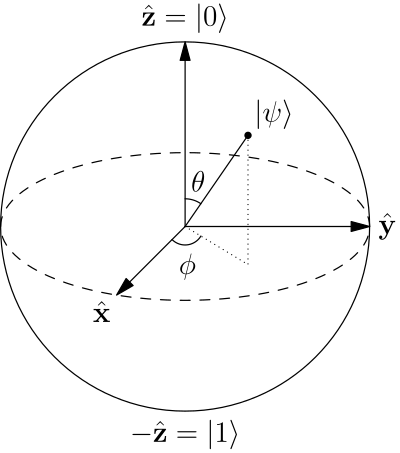
\includegraphics[width = 0.5\textwidth]{Chapters/Graphics/Bloch_Sphere.png}
    \caption{Bloch sphere}
\end{figure}

Suppose we have two qubits then the basis of the system is \(\set{\ket{00}, \ket{01} , \ket{10} , \ket{11}}\) and every state is represent in a superposition of this basis
\begin{equation*}
    \ket{\psi} = \sum_{x \in \set{0,1}^2} \alpha_x \ket{x} \quad \text{with} \quad \sum_{x \in \set{0,1}^2} \abs{\alpha_x}^2 = 1
\end{equation*}
If we measure the first we get \(\ket{0}\) with probability 
\begin{equation*}
    \abs{\alpha_{00}}^2 + \abs{\alpha_{01}}^2 
\end{equation*}
and the post-measurement state would be 
\begin{equation*}
    \ket{\psi'} = \dfrac{\alpha_{00} \ket{00} + \alpha_{01} \ket{01}}{\sqrt{\abs{\alpha_{00}}^2 + \abs{\alpha_{01}}^2}}
\end{equation*}
Bell state or EPR pair is 
\begin{equation*}
    \dfrac{\ket{00} + \ket{11}}{\sqrt{2}}
\end{equation*}
A state of multiple qubit is called \textit{separable} if each of the qubit is in a definite state i.e. we can write it as a tensor product. Otherwise, they are in an \textit{entangled} state.


\section{Quantum gates and measurements}

Isolated quantum mechanic processes (evolution) are represent by unitary matrices \(U U^{\dagger} = I\). Some example of quantum gates include
\begin{align*} 
    \sigma_x &= X = \begin{bmatrix}
        0 & 1 \\
        1 & 0
    \end{bmatrix} \quad \text{Quantum NOT gate}\\
    \sigma_y &= Y = \begin{bmatrix}
        0 & -i \\
        i & 0
    \end{bmatrix} \quad \text{Y gate}\\
    \sigma_z &= Z = \begin{bmatrix}
        1 & 0 \\
        0 & -1
    \end{bmatrix} \quad \text{Z gate}\\
    H &= \dfrac{1}{\sqrt{2}} \begin{bmatrix}
        1 & 1 \\
        1 & -1
    \end{bmatrix} \quad \text{Hadamard gate}\\
\end{align*}
The first three gate correspond to \(180^{\circ}\) rotation along the \(x,y,\) and \(z\) respectively, and are called the \textit{Pauli rotation matrices}. Every gate on a qubit can be viewed as a set of rotations along the \(x,y,z\)-axis of the Bloch sphere. Furthermore, every unitary matrix can be viewed geomtrically as scaling-rotation-scaling. A \textit{Controlled NOT} gate is a two qubit gate 
\begin{figure}
    \centering
    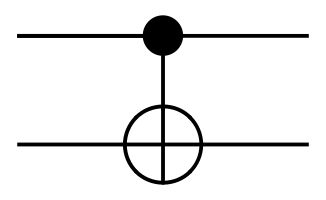
\includegraphics[width = 0.3\textwidth]{Chapters/Graphics/CNOT_Gate.png}
    \caption{CNOT gate}
\end{figure}
that given \(\ket{\psi} \) and \(\ket{\phi}\) input, gives \(\ket{\psi}\) and \(\ket{\psi \oplus \phi}\). The matrix of CNOT gate is 
\begin{equation*}
    U_{CNOT}  = \begin{bmatrix}
        1 & 0 & 0 & 0 \\
        0 & 1 & 0 & 0 \\
        0 & 0 & 0 & 1 \\
        0 & 0 & 1 & 0 \\
    \end{bmatrix}
\end{equation*}

Quantum gates need to be reversible, that is given the output one can find out the output. For example, classical NOT gate is reversible and XOR gate is non-reversible. All multiple qubit gate may be decomposed to CNOT and other single qubit gates. Feedback, FANIN (irreversible) , FANOUT (cloning) are not allowed in quantum computing. In general, Controlled-\(U\) gate is shown as
\begin{figure}
    \centering
    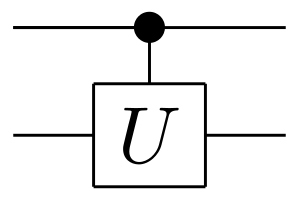
\includegraphics[width = 0.3\textwidth]{Chapters/Graphics/Controlled_Gate.png}
    \caption{Controlled-\(U\) gate}
\end{figure}
and has matrix representation
\begin{equation*}
    \text{Controlled} U = \begin{bmatrix}
        I_n & 0 \\
        0 & U \\
    \end{bmatrix}
\end{equation*}
and measurement of a quantum state is represent by 
\begin{figure}
    \centering
    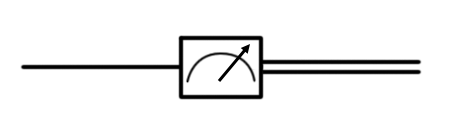
\includegraphics[width = 0.3\textwidth]{Chapters/Graphics/Measurement.png}
    \caption{Measurement}
\end{figure}

No cloning theorem states that lossless copying of qubit using unitary devices can obly be done on orthogonal basis. That is, if \(\ket{\psi}\) can be copied to \(\ket{\phi}\) then 
\begin{equation*}
    \braket{\phi}{\psi} = \begin{cases}
        0 & \psi \perp \phi\\
        1 & \psi = \phi
    \end{cases}
\end{equation*}


\section{Quantum teleportation}
The other Bell states are 
\begin{align*}
    \ket{\beta_{00}} &= \dfrac{\ket{00} + \ket{11}}{\sqrt{2}}\\
    \ket{\beta_{01}} &= \dfrac{\ket{01} + \ket{10}}{\sqrt{2}}\\
    \ket{\beta_{10}} &= \dfrac{\ket{00} - \ket{11}}{\sqrt{2}}\\
    \ket{\beta_{11}} &= \dfrac{\ket{01} - \ket{10}}{\sqrt{2}}
\end{align*}
which are generated by the following circuit --insert diagram Hadamard on the frist qubit and CNOT on the second 
with matrix 
\begin{equation*}
    U = \begin{bmatrix}
        \frac{1}{\sqrt{2}} & 0 & \frac{1}{\sqrt{2}} & 0\\
        0 & \frac{1}{\sqrt{2}} & 0 & \frac{1}{\sqrt{2}} \\
        0 & \frac{1}{\sqrt{2}} & 0 & -\frac{1}{\sqrt{2}} \\
        \frac{1}{\sqrt{2}} & 0 & - \frac{1}{\sqrt{2}} & 0
    \end{bmatrix} = \begin{bmatrix}
        \ket{\beta_{00}} & \ket{\beta_{01}} & \ket{\beta_{10}} & \ket{\beta_{11}}
    \end{bmatrix}
\end{equation*}
Suppose Alice and Bob have an EPR pair \(\ket{\beta_{00}}\), and each took one the pairs. Alice then wants to communicate to Bob the state \(\ket{\psi}\) using only classical bit. Alice and Bob can implement the following -- insert diagram CNOT on Alice qubit, Hadamard on psi, measure psi and alice qubit, not gate on bob and measured alice and Z gate on bob and measure psi. 
\begin{align*}
    \ket{\psi_0} &= \dfrac{\alpha \ket{0} \bracket{\ket{00} + \ket{11}} +  \beta \ket{1} \bracket{\ket{00} + \ket{11}}}{\sqrt{2}}\\
    \ket{\psi_1} &= \dfrac{\alpha \ket{0} \bracket{\ket{00} + \ket{11}} +  \beta \ket{1} \bracket{\ket{10} + \ket{01}}}{\sqrt{2}}\\
    \ket{\psi_2} &= \dfrac{\alpha \ket{+} \bracket{\ket{00} + \ket{11}} +  \beta \ket{-} \bracket{\ket{00} + \ket{11}}}{\sqrt{2}}\\
    &=  \dfrac{1}{2} \ket{00} \bracket{\alpha \ket{0} + \beta \ket{1}} + \dfrac{1}{2} \ket{01} \bracket{\beta \ket{0} + \alpha \ket{1}} \\ \quad &+ \dfrac{1}{2} \ket{10} \bracket{\alpha \ket{0} - \beta \ket{1}} + \dfrac{1}{2} \ket{11} \bracket{\beta \ket{0} - \alpha \ket{1}}\\
    &= \dfrac{1}{2} \ket{00}  \ket{\psi} + \dfrac{1}{2} \ket{01}  \ket{X\psi} + \dfrac{1}{2} \ket{10}  \ket{Z\psi} + \dfrac{1}{2} \ket{11}  \ket{XZ\psi}
\end{align*}
Therefore, after measurements and applying X and Z gates, Bob will have \(\ket{\psi}\). Quantum teleportation is related to quantum erroc correcting codes.

\section{Reversible computing}
A Turing machine \(\calM\) is said to be reversible if there exists another Turing machine \(\calM'\) such that for every configuration change \(c \to c'\) in \(\calM\), there is the configuration change \(c' \to c\) in \(\calM'\).

\begin{theorem}[Bennett 1973]
    For every function \(f\) computable by a one-tape Turing machine in time \(\func{t}{n}\), there is a three-tape reversible Turing machine computing the following mapping within a constant time overhead.
    \begin{equation*}
        a \mapsto (a,\func{j}{a}, \func{f}{a})
    \end{equation*}
    where \(\func{j}{a}\) is ``garbage''. To remove the garbage
    \begin{description}
        \item [Compute \(f\):] \(a \mapsto (a,\func{j}{a}, \func{f}{a})\).
        \item [Fanout: ]\( (a,\func{j}{a}, \func{f}{a}) \mapsto (a,\func{j}{a}, \func{f}{a},\func{f}{a})\).
        \item [Uncompute \(f\):] \( ( (a,\func{j}{a}, \func{f}{a},\func{f}{a}) \mapsto (a,\func{f}{a})\).
    \end{description}
\end{theorem}

Can Quantum computer simulat classical circuits? Yes; since any classical circuit can be replaced by reversible elements such as Toffoli gate (--insert diagram for Toffoli gate, NAND , and FANOUT). The matrix representation of Toffoli gate 
\begin{equation*}
    U = \begin{bmatrix}
        1 & 0 & 0 & 0 & 0 & 0 &0 & 0\\
        0 & 1 & 0 & 0 & 0 & 0 &0 & 0\\
        0 & 0 & 1 & 0 & 0 & 0 &0 & 0\\
        0 & 0 & 0 & 1 & 0 & 0 &0 & 0\\
        0 & 0 & 0 & 0 & 1 & 0 &0 & 0\\
        0 & 0 & 0 & 0 & 0 & 1 &0 & 0\\
        0 & 0 & 0 & 0 & 0 & 0 &0 & 1\\
        1 & 0 & 0 & 0 & 0 & 0 &1 & 0\\
    \end{bmatrix}
    = \begin{bmatrix}
        I_6 & 0 \\
        0 & X\\
    \end{bmatrix}
\end{equation*}
Note that FANOUT creates entangled copies of the quantum state hence it does not violate the no cloning theorems.
We can even assume that classical computer can make random bit. It is easy to see that by using Hadamard gate and then measuring it, quantum computers can make random bits. --insert diagram

\section{Quantum Algorithms and parallelism}
Let \(f : \set{0,1} \to \set{0,1}\) and \(U_f\) be \(\ket{x,y} \mapsto \ket{x, \func{f}{x} \oplus y}\).
\begin{equation*}
    U_f = \begin{bmatrix}
        \func{f'}{0} & \func{f}{0} & 0 & 0\\
        \func{f}{0} & \func{f'}{0} & 0 & 0\\
        0 & 0 & \func{f'}{1} & \func{f}{1}\\
        0 & 0 \func{f}{1} & \func{f'}{1} 
    \end{bmatrix}
\end{equation*}
--insert diagram of Uf and Hadamard
Applying \(\ket{+,0}\) to \(U_f\) gives 
\begin{align*}
    U_f \ket{+,0} &= \dfrac{1}{\sqrt{2}} U_f \ket{00} +  \dfrac{1}{\sqrt{2}} U_f \ket{10}\\
    &= \dfrac{1}{\sqrt{2}} \bracket{\func{f'}{0}\ket{00} + \func{f}{0}\ket{01}} + \dfrac{1}{\sqrt{2}} \bracket{\func{f'}{1}\ket{10} + \func{f}{1}\ket{11}}\\
    &= \dfrac{\ket{0,\func{f}{0}} + \ket{1,\func{f}{1}}}{\sqrt{2}}
\end{align*}
Hence, with a single operation we can "evaluate" \(f\) for all values. Using Hadamard-Welsh Transform we can do this for any function.
\subsection{Deutsch Algorithm}

Let \(f : \set{0,1}^n \to \set{0,1}\) with \(U_f\). Similar to parallelism is one-bit case we can have 
\begin{equation*}
    U_f \ket{0\dots0 , 0} = \dfrac{1}{\sqrt{2^n}} \sum_{x \in \set{0,1}^n} \ket{x} \otimes \ket{\func{f}{x}}
\end{equation*}
using inference property/ measure (will be like the classical case) we can extract information about \(f\). For example, in Deutsch algorithm we use \(U_f\) and construct the following --insert diagram 
\begin{align*}
    \ket{\psi_0} &= \ket{01} \\
    \ket{\psi_1} &= \dfrac{1}{2} \bracket{\ket{00} + \ket{01} + \ket{10}+ \ket{11}}\\
    \ket{\psi_2} &= U_f \ket{\psi_1} \\
    &= \dfrac{1}{2} \begin{bmatrix}
        \func{f'}{0} - \func{f}{0}\\
        \func{f}{0} - \func{f'}{0}\\
        \func{f'}{1} - \func{f}{1}\\
        \func{f}{1} - \func{f'}{1}
    \end{bmatrix}
    \intertext{let \(p_0 = \func{f'}{0} - \func{f}{0}\) and \(p_1 \func{f'}{1} - \func{f}{1}\) then}
    &= \dfrac{1}{2} \bracket{p_0 \ket{00} - p_0 \ket{01} + p_1 \ket{10} - p_1 \ket{11}}\\
    &= \dfrac{1}{2} \bracket{p_0 \ket{0} + p_1 \ket{1}} \otimes \bracket{\ket{0} - \ket{1}} \\
    &= \begin{cases}
        (-1)^{\func{f}{0}} \ket{+} \otimes \ket{-} & \func{f}{0} = \func{f}{1} \\
        (-1)^{\func{f}{0}} \ket{-} \otimes \ket{-} & \func{f}{0} \neq \func{f}{1} 
    \end{cases}\\
    \ket{\psi_3} &= \begin{cases}
        (-1)^{\func{f}{0}} \ket{0} \otimes \ket{-} & \func{f}{0} = \func{f}{1} \\
        (-1)^{\func{f}{0}} \ket{1} \otimes \ket{-} & \func{f}{0} \neq \func{f}{1} 
    \end{cases}\\
    &= (-1)^{\func{f}{0}} \ket{\func{f}{0} \oplus \func{f}{1}} \otimes \ket{-} 
\end{align*}
hence in one operation we can learn a global property of the function namely the value of \(\func{f}{0} \oplus \func{f}{1}\). A generalization of Deutsch algorithm is the Deutsch-Jozsa algorithm which extends \(f : \set{0,1}^n \to \set{0,1}\). First, consider the \(n\)-qubit Hadamard gate is defined as 
\begin{align*}
    H^{\otimes n} \ket{x_1, \dots, x_n} &= H \ket{x_1} \otimes \dots \otimes H \ket{x_n}\\
    &= \dfrac{1}{\sqrt{2^n}} \sum_{z \in \set{0,1}^n} (-1)^{x \cdot z} \ket{z}
\end{align*}
where \(x \cdot z = x_1z_1 + x_2 z_2 + \dots + x_n z_n\). In particular 
\begin{align*}
    H^{\otimes n} \ket{0 \dots 0} &= \dfrac{1}{\sqrt{2^n}} \bracket{ \ket{0}  + \ket{1}} \otimes \dots \otimes \bracket{\ket{0} + \ket{1}}\\
    &= \dfrac{1}{\sqrt{2^n}} \sum_{x \in \set{0,1}^n} \ket{x}\\
\end{align*}
The Deutsch-Jozsa algorithm works as follow --insert diagram 
\begin{align*}
    \ket{\psi_0} &= \ket{0\dots 0, 1}\\
    \ket{\psi_1} &= \ket{+ \dots +, -} = \dfrac{1}{\sqrt{2^n}} \bracket{\sum_{x \in \set{0,1}^n} \ket{x} } \otimes \ket{-}\\ 
    \ket{\psi_2} &= \dfrac{1}{\sqrt{2^n}} \bracket{\sum_{x \in \set{0,1}^n} (-1)^{\func{f}{x}}\ket{x} } \otimes \ket{-}\\
    \ket{\psi_3} &= \dfrac{1}{2^n} \bracket{\sum_{z \in \set{0,1}^n} \sum_{x \in \set{0,1}^n}  (-1)^{\func{f}{x} + x \cdot z} \ket{z}} \otimes \ket{-}
\end{align*}
Now we can determine whether \(f\) is constant or balance (has the same number of one and zeros) by measuring the first qubit. 
\begin{itemize}
    \item If \(f\) is constant then the amplitude of the first bit is \(1\).
    \item If \(f\) is balanced then the amplitude of the first bit is \(0\).
\end{itemize}
Hence after measuring if \(\ket{0}\) then \(f\) is constant, otherwise \(f\) is balanced. 


\subsection{Quantum algorithms on Fourier}
such as Deutsch-Jozsa and Shor's algorithms. The Fourier transform
\begin{equation*}
    \ket{j} \mapsto \dfrac{1}{\sqrt{2^n}} \sum_{k = 0}^{2^n - 1} e^{2\pi i \frac{jk}{2^n}} \ket{k}
\end{equation*}
is a unitary operation. Fast Fourier transform on classical is \(\bigO{N \lg N}\) and on quantum is \(\bigO{\lg^2 N}\). The quantum Fourier transform and Shor's algorithm can be used to solve a class of problems, the \textit{hidden subgroup problem}. Suppose \(f: G \to X\), where \(G\) is a finitely generated group and \(X\) is a finite set, is such that \(f\) is constant and distinct on the cosets of subgroup \(K\). Given a quantum black box for performing the unitary transformation \(U \ket{g} \ket{h} = \ket{g} \ket{h \oplus \func{f}{g}}\) for \(g \in G\), \(h \in X\), and \(\oplus\) is an appropriately chose binary operation on \(X\), find a generating set for \(K\).

\subsection{Quantum search algorithms}
Such as Grover's algorithm.
Given a set \(S\) of \(N\) points and a property \(P\), find \(n \in S\) such that \(\func{p}{n}\). On classical it can be done in \(\bigO{N}\) but quantum search algorithms are able to do it in \(\bigO{\sqrt{N}}\), a quadratic speed up.
\subsection{Quantum simulation}
\(c^n\) on classical but \(cn\) on quantum, however there is hidden information.
\section{Stern-Gerlach experiment}
Quantum tomography, determining the quantum state of a system.
At small scaled optical techniques have been used to certain degree of success. ion-trap, neutral atom trap, quantum jump, nuclear magnetic resonance (NMR).

\section{Quantum information theory}
\begin{enumerate}
    \item Identify elementary classes of static resources in quantum mechanic, e.g. qubit.
    \item Identify elementary classes of dynamic processes in quantum mechanic, e.g. memory
    \item Quantify resource trade-offs in \(\ast\) current performan dynamic processes.
\end{enumerate}
\subsection{Shannon's noisy/noiseless channel coding theorem}
\begin{itemize}
    \item HSW (Holeve, Shunmacher, Westareland) theorem
    \item Shunmacher's noiseless channel coding theorem
    \item von Neumann entropy agrees with Shannon's entropy if the states are orthogonal. Strictly smaller because of redundancy in non-orthogonal states.
\end{itemize}


Cryptography : Kah96, MooV96, Sch 96a, DL 98 
teleporation and NMR: BBC+93, BBM+ 98, BPM+ 97 , FSB+ 98, NKL 98
\chapter{Linear Algebra}
A system in quantum mechanic is modeled by a Hilbert space \(\calH\), which is a complete complex inner product space. The states correspond to vectors in the Hilbert space and are denoted by \(\ket{\psi}\). The conjugate transpose of a state is \(\bra{\psi} = \ket{\psi}^{\dagger}\). The inner product is defined as \(\angleBracket{\phi,\psi} = \braket{\phi}{\psi}\) and hence the norm is  
\begin{equation*}
    \norm{\ket{\psi}} = \sqrt{\braket{\psi}{\psi}}
\end{equation*}
We can define linear operator \(A : \calH \to \calH\), \(A \in \func{\calL}{\calH}\). \(A\) is said to be positive (positive semi-,negative semi-,negative) definite if for all \(\ket{\psi} \in \calH\), \(\bra{\psi} A \ket{\psi} > ( \geq , \leq , <)0\). The norm of an operator is defined as 
\begin{equation*}
    \norm{A} = \sup_{\norm{\ket{\psi}} = 1} \norm{A \ket{\psi}}
\end{equation*}
For example, the Pauli matrices are \(\squareMatrices[\Complex]{2}\) 
\begin{align*}
    \sigma_0 &= I = \begin{bmatrix}
        1 & 0\\
        0 & 1 
    \end{bmatrix} \qquad &\sigma_1 &= \sigma_x = X = \begin{bmatrix}
        0 & 1 \\
        1 & 0 
    \end{bmatrix}\\
    \sigma_2 &= \sigma_y = Y = \begin{bmatrix}
        0 & -i \\
        i & 0
    \end{bmatrix} \qquad &\sigma_3& = \sigma_z= Z = \begin{bmatrix}
        1 & 0 \\
        0 & -1 
    \end{bmatrix}
\end{align*}
For \(\ket{\psi} \in \calH, \ket{\psi'} \in \calH'\) we can define an outer product \(\ket{\psi'}\bra{\psi} : \calH \to \calH\). 
\begin{equation*}
    \ket{\psi'} \bra{\psi} \ket{\phi} = \braket{\psi}{\phi} \ket{\psi'}
\end{equation*}
The completeness relation says that given an orthogonal basis \(\ket{i}\) 
\begin{equation*}
    \sum_i \ket{i} \bra{i} = I 
\end{equation*}
which is easy to see 
\begin{equation*}
    \sum_i \ket{i} \bra{i} \ket{\psi} = \sum \braket{i}{\psi} \ket{i} = \ket{\psi}
\end{equation*}
In any inner product space the Cauchy-Schwarz inequality holds.
\begin{equation*}
    \braket{\psi}{\psi} \braket{\phi}{\phi} \geq \abs{\braket{\psi}{\phi}}^2
\end{equation*}

\section{Adjoint and Hermitian operators}
For any linear operator on a Hilbert space there exists \(B\) such that for all \(\ket{\psi}, \ket{\phi}\in \calH\) 
\begin{equation*}
    \braket{\psi}{A\phi} = \braket{B\psi}{\phi}
\end{equation*}
It is easy to see that \(B = A^{\dagger}\) the adjoint or Hermitian conjuagate of \(A\). \(A = A^{\dagger}\) is a Hermitian or self-adjoint operator. A projection is an operator that projects \(\ket{v}\) into its compenents on a subspace. Suppose \(\ket{1} , \dots , \ket{k}\) is an orthonormal basis for subspace \(W\) 
\begin{equation*}
    P = \sum_{i = 1}^k \ket{i} \bra{i}
\end{equation*}
Geoemtrically, applying \(P\) twice to a vector should again give the projection of that vector that is, \(P^2 = P\). 
\begin{align*}
    P^2 &=  \bracket{\sum_{i = 1}^k \ket{i} \bra{i}}  \bracket{\sum_{j = 1}^k \ket{j} \bra{j}}\\
    &=  \sum_{i = 1}^k  \sum_{j = 1}^k \ket{i} \bra{i} \ket{j} \bra{j} \\
    &=  \sum_{i = 1}^k  \sum_{j = 1}^k \ket{i} \braket{i}{j} \bra{j} \\
    &= \sum_{i = 1}^k \ket{i} \braket{i}{i} \bra{i} \\
    &=  \sum_{i = 1}^k  \ket{i}  \bra{j} = P
\end{align*} 

\(A A^{\dagger} = A^{\dagger} A\) is a normal operator. An operator is diagonalizable if it has a diagonal representation 
\begin{equation*}
    A = \sum \lambda_i \ket{i} \bra{i}
\end{equation*}
where \(\lambda_i\) are the eigenvalues and \(\ket{i}\) form an orthonormal set for the eigenvectors of \(A\). If an eigenspace has dimension greater than one then those eigenvectors are called degenerates.
\begin{theorem}[Spectral decomposition]
    Any normal operator \(M\) is diagonal with respect to orthonormal basis in \(V\). The converse is also true, any diagonalizable matrix is normal.
\end{theorem}

\begin{proof}
    Lets induct over \(\dim V\). If \(\dim V = 1\) then it is trivial that \(M\) is diagonal. Suppose \(\lambda\) is an eigenvalue of \(M\) and \(P\) is the projection onto its eigenspace. Then, \(M = (P + Q) M (P + Q) = PMP + PMQ + QMP + QMQ\) where \(Q = I - P\). Clearly, \(PMP = \lambda P\) and \(QMP = 0\). We claim that \(PMQ = QM^{\dagger} P \) is zero as well. Suppose \(\ket{v} \in P\) then 
    \begin{equation*}
        M \bracket{M^{\dagger} \ket{v}} = M^{\dagger} M \ket{v} = \lambda M^{\dagger} \ket{v}
    \end{equation*}
    Therefore, \(M^{\dagger} \in P\) as well, hence \(PMQ = 0\). We then show that \(QMQ\) is normal as well. 
    \begin{align*}
        \bracket{QMQ} \bracket{QMQ}^{\dagger} &= QMQQM^{\dagger}Q\\
        &= Q M Q M^{\dagger} Q \\
        &= QM M^{\dagger} Q \qquad (QM^{\dagger} = QM^{\dagger} Q + QM^{\dagger} P = QM^{\dagger}Q)\\
        &= QM^{\dagger} M Q \\
        &= QM^{\dagger} QMQ  \qquad (QMQ = MQ - PMQ = MQ)\\
        &= \bracket{QMQ}^{\dagger} \bracket{QMQ}
    \end{align*}
    Now note that \(PMP\) is diagonal with respect to an orthonormal basis for \(P\) and by induction hypothesis there is a basis for \(Q\) such that \(QMP\) is diagonal. Together, these two imply that \(M\) with respect to the union of these two basis is diagonal in \(V\). Furthermore, this implies that \(M\) can be written as 
    \begin{equation*}
        M = \sum \lambda_i \ket{i} \bra{i}
    \end{equation*}
    where \(\lambda_i\) are its eigenvalues. To show that converse, suppose \(M\) is diagonalizable. Then,
    \begin{align*}
        M^{\dagger} M &=\bracket{\sum \lambda_i^{\ast} \ket{i} \bra{i}} \bracket{\sum \lambda_i\ket{i} \bra{i}}\\
        &= \sum_i \sum_j \lambda_i^{\ast} \ket{i} \bra{i}  \lambda_j\ket{j} \bra{j}\\
        &= \sum_i \norm{\lambda}^2 \ket{i} \bra{i}
    \end{align*} 
    and similarly 
    \begin{align*}
        M M^{\dagger}  &=  \bracket{\sum \lambda_i\ket{i} \bra{i}} \bracket{\sum \lambda_i^{\ast} \ket{i} \bra{i}}\\
        &= \sum_i \sum_j \lambda_i \ket{i} \bra{i}  \lambda_j^{\ast} \ket{j} \bra{j}\\
        &= \sum_i \norm{\lambda}^2 \ket{i} \bra{i} \implies M M^{\dagger} = M^{\dagger} M
    \end{align*}
\end{proof}

\begin{theorem}
    A normal operator is hermitian if and only if it has real eigenvalues.
\end{theorem}
\begin{proof}
    A hermitian operator is normal and has real eigenvalues since
    \begin{equation*}
        \bra{v} A \ket{v} = \lambda \braket{v}{v}
    \end{equation*} 
    and 
    \begin{equation*}
        \bra{v} A \ket{v} = \bra{v} A^{\dagger} \ket{v} = \bracket{\bra{v} A \ket{v}}^{\dagger} \implies \lambda = \lambda^{\ast}
    \end{equation*}
    Suppose \(A\) is a normal with real eigenvalues. By spectral decomposition
    \begin{equation*}
        A^{\dagger} = \bracket{\sum \lambda_i \ket{i} \bra{i}}^{\dagger} =  \sum \lambda^{\ast}_i \ket{i} \bra{i} = \sum \lambda_i \ket{i} \bra{i} = A
    \end{equation*}
\end{proof}
\(UU^{\dagger} = I\) is unitary.
\begin{proposition}
    an unitary operator
    \begin{enumerate}
        \item  preserves inner product.
        \item there are two orthonormal basis \(\ket{v_i}, \ket{w_i}\) such that 
        \begin{equation*}
            U = \sum \ket{w_i} \bra{v_i}
        \end{equation*}
        \item its eigenvalues have modulus \(1\)
        
    \end{enumerate}
\end{proposition}
\begin{proof}
    \begin{enumerate}
        \item     
        \begin{equation*}
            \braket{Uv}{Uw} = \bra{v} U^{\dagger}U \ket{w} = \braket{v}{w}
        \end{equation*}
        \item Let \(\ket{v_i}\) be an orthonormal set and \(\ket{w_i} = U \ket{v_i}\). Then, by above's result \(\ket{w_i}\) are orthonormal as well.
        Also note that for any \(v \in V\), \(\braket{v_i}{v} = \bracket{w_i}{Uv}\). Then, 
        \begin{equation*}
            \sum \ket{w_i} \bra{v_i} \ket{v} = \sum \ket{w_i} \braket{v_i}{v} = \sum  \ket{w_i} \braket{w_i}{Uv} = \sum \ket{w_i} \bra{w_i} \ket{Uv} = U \ket{v}
        \end{equation*}
        therefore 
        \begin{equation*}
            U = \sum \ket{w_i} \bra{v_i}
        \end{equation*}
        \item Let \((v,\ket{v})\) be a pair of eigenvalue and eigenvector of \(U\).
        \begin{align*}
            \braket{Uv}{Uv} &= \braket{v}{v}\\
            &= \norm{v}^2 \braket{v}{v} \implies \norm{v} = 1
        \end{align*}
    \end{enumerate}
\end{proof}
\(A\) is positive when for all \(\ket{v}\), \(\bra{v} A \ket{v} \geq 0\) and positive definite if the equality only happens when \(\ket{v} = 0\).
\begin{proposition}
    Any operator \(A\) can be written as \(A = B + iC\) where \(B,C\) are hermitian.
\end{proposition}
\begin{proof}
    Let 
    \begin{equation*}
        B = \dfrac{A + A^{\dagger}}{2} \qquad C = \dfrac{A - A^{\dagger}}{2i}
    \end{equation*}
    then clearly \(A = B + iC\) and both of the hermitian. 
    \begin{equation*}
        B^{\dagger} = \dfrac{A^{\dagger} + A}{2} = B\qquad C^{\dagger} = \dfrac{A^{\dagger} - A}{-2i} = C
    \end{equation*}
\end{proof}
\begin{proposition}
    Positive operators are hermitian. 
\end{proposition}
\begin{proof}
    By the last result \(A = B + iC\) where \(B,C\) are hermitian. Since \(B,C\) are hermitian then they have spectral decomposition
    \begin{equation*}
        B = \sum \lambda_i \ket{v_i}\bra{v_i}  \qquad C = \sum \gamma_j \ket{w_j}\bra{w_j}
    \end{equation*}
    where \(\lambda_i,\gamma_j\) are real numbers. For every \(\ket{v} \in V\)
    \begin{align*}
        \bra{v} B \ket{v} &= \sum \lambda_i \bra{v} \ket{v_i}\bra{v_i} \ket{v} \\
        &= \sum \lambda_i \norm{\braket{v_i}{v}}^2
    \end{align*}
    is a real number. Therefore, since
    \begin{equation*}
        \bra{v} A \ket{v} = \bra{v} B \ket{v}  + i \bra{v} C \ket{v}
    \end{equation*}
    is a real number as well then 
    \begin{equation*}
        \bra{v} C \ket{v} = 0 \qquad \forall \ket{v}
    \end{equation*}
    Then for any \((\gamma_j, \ket{w_j})\)
    \begin{equation*}
        \bra{w_j} C \ket{w_j} = \gamma_j \braket{w_j}{w_j} = 0
    \end{equation*}
    since \(w_j\) are orthonormal then \(\gamma_j = 0\) and hence \(C = 0 \).
\end{proof}
\section{Tensor product}
Let \(\ket{v} \in V\) and \(\ket{w} \in W\) then 
\begin{equation*}
    \ket{v} \otimes \ket{w} = \begin{bmatrix}
        v_1w_1 & v_1w_2 & \dots & v_1w_m \\
        \vdots & \vdots & \ddots & \vdots\\
        v_nw_1 & v_nw_2 & \dots & v_nw_m
    \end{bmatrix}
    \qquad V \otimes W = \set<\ket{v} \otimes \ket{w}>{\ket{v} \in V, \ket{w} \in W}
\end{equation*}
If \(\ket{i}\) and \(\ket{j}\) are orthonormal basis for \(V\) and \(W\) then \(\ket{i} \otimes \ket{j}\) is a basis for \(V \otimes W\). For operators 
\begin{equation*}
    \bracket{A \otimes B } \bracket{\ket{v} \otimes \ket{w}} = A \ket{v} \otimes B \ket{w}
\end{equation*}
with the Kroneker matrix representation
\begin{equation*}
    A \otimes B = \begin{bmatrix}
        A_{11}B & A_{12}B & \dots & A_{1n}B \\
        \vdots & \vdots & \ddots & \vdots\\
        A_{m1}B & A_{m2}B & \dots & A_{mn}B
    \end{bmatrix}
\end{equation*}
If \(A\) is \(m \times n \) and \(B\) is \(p \times q\) then \(A \times B\) is \(mp \times nq\).
\begin{proposition}
    If \(V\) and \(W\) are inner product space, then we can define the following inner product for \(V \otimes W\)
    \begin{equation*}
        \braket{x \otimes y}{u \otimes v}= \braket{x}{u} \braket{y}{v}
    \end{equation*}
\end{proposition}

\begin{proposition} \leavevmode
    \begin{enumerate}
        \item Tensor product of unitary operators is unitary.
        \item Tensor product of hermitian operators is hermitian.
        \item Tensor product of projection operators is projection.
        \item Tensor product of positive operator is positive.
    \end{enumerate}
\end{proposition}
\section{Operator function}
Let \(A\) be a normal operator then 
\begin{equation*}
    \func{f}{A} = \sum \func{f}{\lambda_i} \ket{i}\bra{i}
\end{equation*}

trace of a matrix is the sum of its diagonal elements. 
\begin{equation*}
    \trace A = \sum a_{ii}
\end{equation*}
\begin{proposition}
    \begin{enumerate}
        \item it is commutative 
        \begin{equation*}
            \trace AB =  \trace BA
        \end{equation*}
        \item it is linear 
        \begin{equation*}
            \trace A + cB = \trace A + c \trace B
        \end{equation*}
        \item it is invariant under unitary transformation
        \begin{equation*}
            \trace U A U^{\dagger} = \trace A
        \end{equation*}
    \end{enumerate}
\end{proposition}

\begin{proposition}
    Let \(\func{\calL}{V}\) be all the linear function on \(V\). Give a basis for \(\func{\calL}{V}\) and show that 
    \begin{equation*}
        \angleBracket{A,B} = \trace A^{\dagger}B
    \end{equation*}
    is an inner product. Find a basis for hermitian matrices for \(\func{\calL}{V}\).
\end{proposition}

\section{Commutators and anti-commutators}
\begin{equation*}
    \squareBracket{A,B} = AB - BA  \qquad \curlyBracket{A,B} = AB + BA
\end{equation*}
\begin{theorem}[Simultaneous diagonalization theorem] Suppose \(A\) and \(B\) are hermitian. They commute if and only if there exists an orthonormal basis such that \(A\) and \(B\) are both diagonalizable with respect to that basis.
\end{theorem}

\section{Polar decomposition and SVD}
\begin{theorem}
    Let \(A\) be a linear operator on \(V\). There exists an unitary operator and positive operators \(J\) and \(K\) such that 
    \begin{equation*}
        A = UJ = KU
    \end{equation*}
    \(UJ\) is the left PD and \(KU\) is the right PD. \(J,K\) are unique and defined by \(J = \sqrt{A^{\dagger }A}\) and \(L = \sqrt{AA^{\dagger}}\). If \(A\) is invertible then \(U\) is unique. 
\end{theorem}

\begin{theorem}
    Let \(A\) be a square matrix. There are unitary matrices \(U,V\) and diagonal matrix \(D\) with non-negative entries such that 
    \begin{equation*}
        A = UDV
    \end{equation*}
\end{theorem}
\begin{proof}
    By PD, \(A = SJ\) and from spectral theorem \(J = TDT^{\dagger}\) where \(T\) is unitary and \(D\) is diagonal. Therefore \(A = U D T^{\dagger}\) where \(U = ST\).
\end{proof}

\chapter{Quantum Mechanic}
\section{Axioms of quantum mechanic}
Each physical system is a seperable complex Hilbert space -- complete vector space -- with inner product \(\angleBracket{\psi,\phi}\). Rays -- complex subspaces of dimesion 1 -- in \(\calH\) are associated with quantum state of the system. We bring an incomplete set of quantum mechanic axioms.

\begin{description}
    \item [Postulate I:] The state of an isolated physical system at a fixed time \(t\) is represented by a (unit) stated vector \(\ket{\psi}\) belongin to \(\calH\).
    \item [Postulate II:] The evolution of a closed quantum system is described by a unitary transformation.
    \begin{equation*}
        \ket{\psi_{t_1}} = U \ket{\psi_{t_0}}
    \end{equation*}
    The time evolution of the state of a closed quantum system is described by Schrodinger's equation.
    \begin{equation*}
        ih \dfrac{\diffOperator}{\diffOperator t} \ket{\psi} = H \ket{\psi}
    \end{equation*}
    where \(H\) is the Hamiltonian operator. The Hamiltonian is a hermitian operator -- \(H = H^{\dagger}\)-- and it can be decomposed into its energy levels (eigenvalues).
    \begin{equation*}
        H = \sum_{E} E \ket{E} \bra{E}
    \end{equation*}

    \item [Postulate III:] Quantum measurements are described by a collection  of measurement operators \(\set{\calM_m}\) satisfying the completeness relation
    \begin{equation*}
        \sum \calM_m^{\dagger} \calM_m = I
    \end{equation*}
    These are operators acting on the state space of the system being measured.
    \begin{equation*}
        \prob{m} = \bra{\psi} \calM_m^{\dagger} \calM_m \ket{\psi}
    \end{equation*} 
    is the probability of measuring \(m\). \(\set{\calM_m}\) are basically the eigenvectors of a hermitian operator -- therefore, \(\calM_m^{\dagger} \calM_m \) is the eigenspace. The state of quantum system post measurement is 
    \begin{equation*}
        \dfrac{\calM_m \ket{\psi}}{\sqrt{\bra{\psi} \calM_m^{\dagger} \calM_m \ket{\psi}}}
    \end{equation*}
    \item [Postulate IV:] The composite state space is the tensor product of the state spaces of the component physical  systems.
\end{description}

\begin{remark}
    Non-orthogonal states can not be reliably distinguished. Suppose there is a measurement device that can distinguish non-orthogonal states \(\ket{\psi_1}, \ket{\psi_2}\). Suppose \(\ket{\psi_b}\) is prepared, then the probability of measuring \(j\) such that \(\func{f}{j} = b\) is 1. Define 
    \begin{equation*}
        E_i = \sum_{j; \func{f}{j} = i} 
    \end{equation*}
\end{remark}
\section{Projective measurements}
A projective measurement is described by an observable, \(M\), a hermitian operator on the state space of the system being observed.
\begin{equation*}
    M = \sum m P_m
\end{equation*}
where \(P_m\) is the projectors into eigenspace with \(P_i P_j = \delta_{ij} P_i\). Then, the probability of getting result \(m\) is 
\begin{equation*}
    \prob{m} = \bra{\psi} P_m \ket{\psi}
\end{equation*}
We define the average and variance of a projective measurement as follows.
\begin{align*}
    \angleBracket{M} &= \expected{M} = \sum m \prob{m} \\
    &= \sum m \bra{\psi} P_m \ket{\psi} \\
    &= \bra{\psi} \bracket{\sum m P_M} \ket{\psi}\\
    &= \bra{\psi} M \ket{\psi}\\
    \bracket{\Delta M}^2 &= \angleBracket{\bracket{M - \angleBracket{M}}^2}\\
    &= \angleBracket{M^2} - \angleBracket{M}^2
\end{align*}

\begin{remark}[Heisenberg uncertainty principle]
    Suppose \(\ket{\psi}\) is a quantum state and \(A,B\) are hermitian operators. Let 
    \begin{equation*}
        x + iy = \bra{\psi} AB \ket{\psi}
    \end{equation*}
    then, 
    \begin{equation*}
        \bra{\psi} BA \ket{\psi} = \bra{\psi} \bracket{AB}^{\dagger} \ket{\psi} = \bracket{ \bra{\psi} AB \ket{\psi}}^{\dagger} = x - iy
    \end{equation*}
    therefore, 
    \begin{equation*}
        \abs{\bra{\psi} \squareBracket{A,B} \ket{\psi}} = 2\abs{x} \leq 2 \abs{\bra{\psi} AB \ket{\psi}}
    \end{equation*}
    With Cauchy-Schwarz inequality (\(\abs{\bra{\psi}AB \ket{\psi}}\) is an inner product over the space of hermitian operators)
    \begin{align*}
        \abs{\bra{\psi} AB \ket{\psi}}^2 &\leq \bra{\psi} A^2 \ket{\psi} \bra{\psi} B^2 \ket{\psi}\\
        \implies \abs{\bra{\psi} \squareBracket{A,B} \ket{\psi}}^2 &\leq 4  \bra{\psi} B^2 \ket{\psi} \bra{\psi} A^2 \ket{\psi}
    \end{align*}
    Hence if we let \(A = C - \angleBracket{C}, B = D - \angleBracket{D}\) then 
    \begin{align*}
        \squareBracket{A,B} &= \squareBracket{C,D} \\
        \angleBracket{A^2} &= \bracket{\Delta C}^2 , \angleBracket{B^2} = \bracket{\Delta D}^2
    \end{align*}
    and 
    \begin{equation*}
        \bracket{\Delta C} \bracket{\Delta D} \geq \dfrac{\abs{\bra{\psi} \squareBracket{C,D} \ket{\psi}}}{2}
    \end{equation*}
    Which basically means that if two measurements \(C,D\) do not commute then as the error in measuring one decreases the error in measuring the other one must increase. Hence, there would always be an uncertainty in the exact properties of the system.
\end{remark}
Let \(\vec{v}\) be a direction in \(\Reals^3\) then, the measurement of spin along \(\vec{v}\) is defined as 
\begin{equation*}
    \vec{v} \cdot \vec{\sigma} = v_1 \sigma_1  + v_2 \sigma_2 + v_3 \sigma_3
\end{equation*}
where \(\sigma_i\) are the Pauli matrices.

\section{POVM measurement}
Suppose \(\calM_m\) are measurement operators. Then, 
\begin{equation*}
    E_m = \calM_m^{\dagger} \calM_m
\end{equation*}
are positive and complete -- \(\sum_m E_m = I\) --. The complete set of \(\set{E_m}\) is called ``Positive Operator Valued Measure'' or POVM. We can get the \(\set{\calM_m}\) from \(\set{E_m}\) by letting \(\calM_m = \sqrt{E_m}\).
\begin{example}
    Suppose we want to distinguish between \(\ket{\psi} = \ket{0}\) and \(\ket{\psi_2} = \ket{+}\) with no error. Since these two states are 
\end{example}

\section{Density operator}
Suppose a quantum system is prepared in one of the \(\ket{\psi_i}\) states with probability \(p_i\). The density operator for the system is 
\begin{equation*}
    \rho = \sum p_i \ket{\psi_i} \bra{\psi_i}
\end{equation*}
If the system evolves with unitary matrix \(U\) then the density operator evolves to 
\begin{equation*}
    \rho = \sum p_i \ket{\psi_i} \bra{\psi_i} \xrightarrow{U} \sum p_i U\ket{\psi_i} \bra{\psi_i} U^{\dagger} = U \rho U^{\dagger}
\end{equation*}
Furthermore, if \(\set{\calM_m}\) are a set of measurements then,
\begin{equation*}
    \condProb{m}{i} = \bra{\psi_i} \calM_m^{\dagger} \calM_m \ket{\psi_i} = \func{\trace}{ \calM_m^{\dagger} \calM_m \ket{\psi_i} \bra{\psi_i}}
\end{equation*}
and 
\begin{align*}
    \prob{m} &= \sum p_i \condProb{m}{i}\\
    &= \sum p_i \func{\trace}{ \calM_m^{\dagger} \calM_m \ket{\psi_i} \bra{\psi_i}} \\
    &= \func{\trace}{ \calM_m^{\dagger} \calM_m \sum p_i \ket{\psi_i} \bra{\psi_i}} \\
    &= \func{\trace}{ \calM_m^{\dagger} \calM_m \rho}
\end{align*}
If \(m\) was measured in \(\ket{\psi}\) then the post measurement state is 
\begin{equation*}
    \ket{\psi_i^m} = \dfrac{\calM_m \ket{\psi}}{\sqrt{ \func{\trace}{ \calM_m^{\dagger} \calM_m \ket{\psi_i} \bra{\psi_i}}}}
\end{equation*}
and the density operator post measurement is 
\begin{align*}
    \rho_m &= \sum \condProb{i}{m} \ket{\psi_i^m} \bra{\psi_i^m}\\
    &= \sum \bracket{\dfrac{p_i \func{\trace}{ \calM_m^{\dagger} \calM_m \ket{\psi_i} \bra{\psi_i}}}{\func{\trace}{ \calM_m^{\dagger} \calM_m \rho}}} \bracket{\dfrac{\calM_m \ket{\psi_i} \bra{\psi_i} \calM_m^{\dagger}}{\func{\trace}{ \calM_m^{\dagger} \calM_m \ket{\psi_i} \bra{\psi_i}}}}\\
    &= \dfrac{1}{\func{\trace}{ \calM_m^{\dagger} \calM_m \rho}} \sum  p_i \calM_m \ket{\psi_i} \bra{\psi_i} \calM_m^{\dagger}\\
    &= \dfrac{\calM_m \rho \calM_m^{\dagger}}{\func{\trace}{  \calM_m \rho \calM_m^{\dagger}}}
\end{align*}

\begin{theorem}
    An operator \(\rho\) is the density operator associated to some ensemble \(\set{p_i , \ket{\psi_i}}\) if and only if it satisfies the following conditions
    \begin{enumerate}
        \item \(\func{\trace}{\rho} = 1\).
        \item \(\rho\) is a positive operator.
    \end{enumerate}
\end{theorem}

We can reform the quantum mechanic postulate for density operator as follows.
\begin{definition}
    \item [Postulate I:] The state of an isolated physical system at a fixed time \(t\) is completely described by its density operator.
    \item [Postulate II:] The evolution of a closed quantum system is described by a unitary transformation.
    \begin{equation*}
        \rho_{t_1} = U \rho_{t_0} U^{\dagger}
    \end{equation*}
    
    \item [Postulate III:] Quantum measurements are described by a collection \(\set{\calM_m}\) of measurement operators satisfying the completeness relation
    \begin{equation*}
        \sum \calM_m^{\dagger} \calM_m = I
    \end{equation*}
    These are operators acting on the density operator of the system being measured.
    \begin{equation*}
        \prob{m} = \func{\trace}{\calM_m \rho \calM_m^{\dagger}}
    \end{equation*} 
    is the probability of measuring \(m\). \(\set{\calM_m}\) are basically the eigenvectors of a hermitian operator -- therefore, \(\calM_m^{\dagger} \calM_m \) is the eigenspace. The stated post measurement is 
    \begin{equation*}
        \dfrac{\calM_m \rho \calM_m^{\dagger}}{ \func{\trace}{\calM_m \rho \calM_m^{\dagger}}}
    \end{equation*}
    \item [Postulate IV:] The composite density operator is the tensor product of the density operator of the component physical  systems.
    \begin{equation*}
        \rho = \rho_1 \otimes \rho_2 \otimes \dots \otimes \rho_n
    \end{equation*}
\end{definition}

The mean of an operator over a system described by \(\rho\) is 
\begin{align*}
    \angleBracket{A} &= \sum p_i \bra{\psi_i} A \ket{\psi_i} \\
    &= \sum p_i \func{\trace}{A \ket{\psi_i} \bra{\psi_i}}\\
    &= \func{\trace}{A \rho}
\end{align*}

\begin{theorem}
    \(\func{\trace}{\rho^2} \leq 1\), equallity if and only if \(\rho\) is a pure state.
\end{theorem}
\(\ket{\tilde{\psi_i}}\) generates \(\rho\) if \(\rho = \sum_{i} \ket{\tilde{\psi_i}} \bra{\tilde{\psi}_i}\).
\begin{theorem}[Unitary freedon in the ensemble for density matrices]
    Suppose the states \(\ket{\tilde{\psi}_i}\) and \(\ket{\tilde{\phi}_i}\) generate the same density operator if and only if 
    \begin{equation*}
        \ket{\tilde{\psi}_i} = \sum_{j} u_{ij} \ket{\tilde{\phi}_i}
    \end{equation*}
    where \(U = \begin{bmatrix}
        u_{ij}
    \end{bmatrix}\) is a unitary matrix.
\end{theorem}
 \subsection{Reduced density operator}
 \(\rho^{AB}\) is  density operator for systems \(A\) and \(B\). The reduced density operator for system \(A\) is 
 \begin{equation*}
    \rho^Q = \func{\trace_B}{\rho^{AB}}
 \end{equation*}
 where 
 \begin{equation*}
    \func{\trace_B}{\ket{a_1}\bra{a_2} \otimes \ket{b_1}\bra{b_2}} = \func{\trace}{\ket{b_1}\bra{b_2}}\ket{a_1}\bra{a_2} + \bra{b_1}\ket{b_2}\ket{a_1}\bra{a_2} 
 \end{equation*}

 \begin{theorem}[Schmidt Decompostion]
    Suppose \(\ket{\psi}\) is a pure state of a composite systems \(A\) and \(B\). There exists an orthonormal states \(\ket{i_A}\) for the system \(A\) and orthonormal states \(\ket{i_B}\) for system \(B\) such that 
    \begin{equation*}
        \ket{\psi} = \sum_i \lambda_i \ket{i_A} \ket{i_B}
    \end{equation*}
    where \(\lambda_i \geq 0\) satisfying \(\sum_i \lambda_i^2 = 1\) known as Schmidt coefficients. The number of non-zero values of \(\lambda_i\) is called the Schmidt number.
 \end{theorem}
 \begin{definition}[Purifiction]
    \(\rho^A\) of a quantum system \(A\). It is possible to introduce another system whcih we donte by \(R\), the reference system, and define a pure state \(\ket{AR}\) reduces to \(\rho^A\)
 \end{definition}

 \section{Bell's inequality}

 \section{Extra}
 \begin{theorem}
    If a state \(\ket{\psi}\) of a Hilbert space of \(n\) qubits can be written as a superposition of \(m_1\) basis in standart basis and \(m_2\) basis in the dual basis, then 
    \begin{equation*}
        m_1 m_2 \geq 2^n
    \end{equation*}
 \end{theorem}
 The amount of entanglement in a pure state \(\ket{\psi}\) of a compound system \(A \otimes B\) is measured by
 \begin{equation*}
    \func{E}{\psi} = - \func{\trace}{\rho_A \lg \rho_A} = - \func{\trace}{\rho_B \lg \rho_B}
 \end{equation*}
 where \(\rho = \ket{\psi} \bra{\psi}\). This is the von-Neumann entropy. A pair of maximally entangled qubits are called ebit. Bell pairs are maximally entangled.
 In \(\calH_n\)
 \begin{equation*}
    \ket{\phi_n} = \dfrac{1}{\sqrt{N}} \sum_{i = 1}^n \ket{i}\ket{i}
 \end{equation*}
is maximally entangled. In \(H_2\) 
\begin{equation*}
    \frac{1}{\sqrt{k}} \ket{00} + \sqrt{\dfrac{k-1}{k}} \ket{11}
\end{equation*}
for large \(k\) is weakly entangled. For mixed states entanglement is defined similarly.
-- multi-party communication
-- Two-party communication complexity.
\chapter{Automaton}
A PTM \(\delta: Q \times \Gamma \times Q \times \Gamma \times \set{L,S,R} \to \clcl{0}{1}\). Local probability condition
\begin{equation*}
    \sum_{(q_d,a_d,d) \in Q \times \Gamma \times \set{L,S,R}} \func{\delta}{q_s,a_s,q_d,a_d,d} = 1
\end{equation*}
Global probability condition: Suppose \(c_1, \dots, c_k\) are distinct possible configuration with probabilities \(p_1, \dots, p_k\) respectively. Then, 
\begin{equation*}
    \sum_{i = 1}^k p_i = 1
\end{equation*}
\begin{proposition}
    Local probability condition gives global probability condition.
\end{proposition}
The Transition matrix is \(M = \begin{bmatrix}
    p_{ij}
\end{bmatrix}\) where \(p_{ij}\) is the probability that \(c_i\) is the successor of \(c_j\).

A QTM \(\delta: Q \times \Gamma \times Q \times \Gamma \times \set{L,S,R} \to \Complex_{\clcl{0}{1}} = \set<z \in \Complex>{\abs{z} \leq 1}\).Local probability condition
\begin{equation*}
    \sum_{(q_d,a_d,d) \in Q \times \Gamma \times \set{L,S,R}} \abs{\func{\delta}{q_s,a_s,q_d,a_d,d}}^2 = 1
\end{equation*}
Global probability condition: Suppose \(c_1, \dots, c_k\) are distinct possible configuration with total amplitudes \(\beta_1, \dots, \beta_k\) respectively. Then, 
\begin{equation*}
    \sum_{i = 1}^k \abs{\beta_i}^2 = 1
\end{equation*}
The Transition matrix is \(M = \begin{bmatrix}
    \beta_{ij}
\end{bmatrix}\) where \(\beta_{ij}\) is the amplitude that \(c_i\) is the successor of \(c_j\). Furthermore, \(M\) is unitary
\begin{equation*}
    M M^{\dagger} = M^{\dagger} M = I
\end{equation*}

Difference between PTM and QTM: PTM selects a path but QTM continues all paths as a superposition. We can watch (measure) the computation of PTM without affecting it but not for QTM.

\chapter{Complexity Theory}
\section{Models of computation}
\subsection{Turing machines}
is defined by the tuple \((Q,\Sigma, \Gamma, \delta, q_{acc}, q_{rej})\) where \(\delta: Q \times  \Gamma \to Q \times \Gamma \times \set{L,R,S}\).
\subsection{Circuits}
is defined by gates \(f: \set{0,1}^{k} \to \set{0,1}^l\).
\section{Analysis of computation problems}
\begin{definition}[Strong Church-Turing thesis:] 
    Any model of computation can be simulated  on a probabilistic Turing machine with at most a polynomial increase in the number of elementary operations required.
\end{definition}
The language \(L\) is decided by a Turing machine if the machine is able to decide whether the input \(x\) is a member of \(L\)  or not. That is, on any string it halts. For example, if \(L \in \func{TIME}{\func{f}{n}}\), then a Turing machine can decide \(x\) with \(\abs{x} = n\) in time \(\bigO{\func{f}{n}}\). 
\begin{equation*}
    P = \set<L>{L \in \func{TIME}{n^k}, \; \text{for some finite} \ k}
\end{equation*}
NP are the set of problems not in \(P\) but it can be checked efficiently.
\begin{equation*}
    NP = \set<L>{}
\end{equation*}
%\exists TM \; \suchThat \; \text{if} \(x \in L\) \text{there exists a witness} \(w\) \; \suchThat \; \(TM\) \text{halts at } \(q_{acc}\) \text{starting at} x. \text{Else for all} w, M \text{halts at } \(q_{rej}\)
coNP is the complement of NP. NP-complete if solves in time \(t\) allows any other problem in NP to be solved in \(\bigO{\func{p}{t}}\).

A language \(B\) is reducible to \(A\), if there exists a Turing machine \(TM\), running in polynomial time given \(x\) outputs \(\func{R}{x}\) such that \(x \in B\) if and only if \(\func{R}{x} \in A\).

\begin{proposition}
    If \(L_1\) is reducible to \(L_2\) and \(L_2\) is reducible to \(L_3\), then \(L_1\) is reducible to \(L_3\).
\end{proposition}

A language \(L\) is complete for a class, if \(L\) is in that class and all other languages in that class are reducible to \(L\).
\begin{example}
    Circuit satisfiability is complete for NP. Cook-Levin problem. Given a Boolean circuit with AND, OR, NOT, determine if there is an assignment which output \(1\).
\end{example}

The focus of quantum computer is NPI problems.
\subsection{Space}
PSPACE is the set of all problems that use polynomial nymber of working bits on a Turing machine. \(P \subset NP \subset PSPACE\). If \(P = PSPACE\), then quantum computers are technically worthless. 
\begin{equation*}
    L \subset P \subset NP \subset PSPACE \subset EXP
\end{equation*}
since \(P \subsetneq EXP\), then at least one the of the inequalities is strict. 
\subsection{Approximate algorithms and MASNP}
Random (bound-error probabilistic) BPP and BPQ. done repeatedly gives correct asnwer using Chernoff bound.
\subsection{Energy}
\begin{theorem}[Landauer's first principle] Suppose a computer erases a single bit. The amount of energy dissipated into environment is at least \(k_B T \ln 2\), \(k_B\) is the Boltzmann constant and \(T\) is the temperature.
\end{theorem}

\begin{theorem}[Landauer's second principle] Suppose a computer erases a single bit of information. The entropy of the environment is increased by at least \(k_B \ln 2\)
\end{theorem}
\subsubsection{Reversible and conservative computation}
Fredkin, Toffoli gates.
Reversible computation is highly sensitive to noise and thus we must use an error-correcting code and then need to delete the redundant information which uses energy by Landauer's principles.

Analog computers comput based on continuous degree of freedom. Therefore, are sensitive to noise and thus we need to reduce the number of states from continuous to discrete and finite.

Kau97,98a,98b, Pap94, Min67, Con72,86.
\chapter{Quantum Information Theory}
von-Neumann entropy of a mixed state \(\psi = \bigoplus \ket{p_i,\phi_i}\) is 
\begin{equation*}
    \func{QS}{\rho_{\ket{\psi}}} = - \func{\trace}{\rho_{\ket{\psi}} \lg \rho_{\ket{\psi}}}
\end{equation*}
where \(\lg \rho_{\ket{\psi}}\) is defined as the matrix \(\begin{bmatrix}
    \lg M^B_{\rho_{\ket{\psi}}}
\end{bmatrix}\)
where \(M^B_{\rho_{\ket{\psi}}}\) is the diagonal matrix representation of \(\rho_{\psi}\).
Suppose \(\calH = \calH_A \otimes \calH_B\) and \(\rho\) is a density operator in \(\calH\). Tracing out ??
\begin{equation*}
    \rho_{\calH_A} = \func{\trace_{\calH_B}}{\rho}
\end{equation*}
Fidelity of two states \(\func{F}{\ket{\psi}, \ket{\phi}} = \abs{\bracket{\psi}{\phi}}^2\).
% \part{Quantum Information}

\chapter{Quantum Information Theory}
The von-Neumann entropy of density matrix \(\rho\) is 
\begin{equation*}
    \func{S}{\rho} = - \func{\trace}{\rho \lg \rho}
\end{equation*}
where \(\lg \rho\) is defined as the matrix \(\begin{bmatrix}
    \lg \rho_D
\end{bmatrix}\)
where \(\rho_D\) is the diagonal matrix representation of \(\rho\).

\begin{proposition}
    The entropy of a pure state is zero.
\end{proposition}
\begin{proof}
    When \(\rho = \ket{\psi}\bra{\psi}\), it can be viewed as a projection onto \(\ket{\psi}\). This projection, with one eigenvalue of \(\lambda = 1\) and rest are zeros. Thus, \(\func{S}{\rho} = - 1 \lg 1 = 0\).
\end{proof}
% \input{Chapters/QuantumCommunication.tex}
% \part{Quantum Machine Learning}
% \part{Quantum Electrodynamic}

\appendix
\chapter{Maxwell's Equations}

\chapter{Lie Groups}
\end{document}
